\documentclass[twoside]{book}

% Packages required by doxygen
\usepackage{calc}
\usepackage{doxygen}
\usepackage{graphicx}
\usepackage[utf8]{inputenc}
\usepackage{makeidx}
\usepackage{multicol}
\usepackage{multirow}
\usepackage{textcomp}
\usepackage[table]{xcolor}

% Font selection
\usepackage[T1]{fontenc}
\usepackage{mathptmx}
\usepackage[scaled=.90]{helvet}
\usepackage{courier}
\usepackage{amssymb}
\usepackage{sectsty}
\renewcommand{\familydefault}{\sfdefault}
\allsectionsfont{%
  \fontseries{bc}\selectfont%
  \color{darkgray}%
}
\renewcommand{\DoxyLabelFont}{%
  \fontseries{bc}\selectfont%
  \color{darkgray}%
}

% Page & text layout
\usepackage{geometry}
\geometry{%
  a4paper,%
  top=2.5cm,%
  bottom=2.5cm,%
  left=2.5cm,%
  right=2.5cm%
}
\tolerance=750
\hfuzz=15pt
\hbadness=750
\setlength{\emergencystretch}{15pt}
\setlength{\parindent}{0cm}
\setlength{\parskip}{0.2cm}
\makeatletter
\renewcommand{\paragraph}{%
  \@startsection{paragraph}{4}{0ex}{-1.0ex}{1.0ex}{%
    \normalfont\normalsize\bfseries\SS@parafont%
  }%
}
\renewcommand{\subparagraph}{%
  \@startsection{subparagraph}{5}{0ex}{-1.0ex}{1.0ex}{%
    \normalfont\normalsize\bfseries\SS@subparafont%
  }%
}
\makeatother

% Headers & footers
\usepackage{fancyhdr}
\pagestyle{fancyplain}
\fancyhead[LE]{\fancyplain{}{\bfseries\thepage}}
\fancyhead[CE]{\fancyplain{}{}}
\fancyhead[RE]{\fancyplain{}{\bfseries\leftmark}}
\fancyhead[LO]{\fancyplain{}{\bfseries\rightmark}}
\fancyhead[CO]{\fancyplain{}{}}
\fancyhead[RO]{\fancyplain{}{\bfseries\thepage}}
\fancyfoot[LE]{\fancyplain{}{}}
\fancyfoot[CE]{\fancyplain{}{}}
\fancyfoot[RE]{\fancyplain{}{\bfseries\scriptsize Generated on Fri Feb 25 2022 15\-:04\-:35 for O\-P by Doxygen }}
\fancyfoot[LO]{\fancyplain{}{\bfseries\scriptsize Generated on Fri Feb 25 2022 15\-:04\-:35 for O\-P by Doxygen }}
\fancyfoot[CO]{\fancyplain{}{}}
\fancyfoot[RO]{\fancyplain{}{}}
\renewcommand{\footrulewidth}{0.4pt}
\renewcommand{\chaptermark}[1]{%
  \markboth{#1}{}%
}
\renewcommand{\sectionmark}[1]{%
  \markright{\thesection\ #1}%
}

% Indices & bibliography
\usepackage{natbib}
\usepackage[titles]{tocloft}
\setcounter{tocdepth}{3}
\setcounter{secnumdepth}{5}
\makeindex

% Hyperlinks (required, but should be loaded last)
\usepackage{ifpdf}
\ifpdf
  \usepackage[pdftex,pagebackref=true]{hyperref}
\else
  \usepackage[ps2pdf,pagebackref=true]{hyperref}
\fi
\hypersetup{%
  colorlinks=true,%
  linkcolor=blue,%
  citecolor=blue,%
  unicode%
}

% Custom commands
\newcommand{\clearemptydoublepage}{%
  \newpage{\pagestyle{empty}\cleardoublepage}%
}


%===== C O N T E N T S =====

\begin{document}

% Titlepage & ToC
\hypersetup{pageanchor=false}
\pagenumbering{roman}
\begin{titlepage}
\vspace*{7cm}
\begin{center}%
{\Large O\-P \\[1ex]\large 0.\-1 }\\
\vspace*{1cm}
{\large Generated by Doxygen 1.8.5}\\
\vspace*{0.5cm}
{\small Fri Feb 25 2022 15:04:35}\\
\end{center}
\end{titlepage}
\clearemptydoublepage
\tableofcontents
\clearemptydoublepage
\pagenumbering{arabic}
\hypersetup{pageanchor=true}

%--- Begin generated contents ---
\chapter{Main Page}
\label{index}\hypertarget{index}{}\input{index}
\chapter{Namespace Index}
\section{Namespace List}
Here is a list of all documented namespaces with brief descriptions\-:\begin{DoxyCompactList}
\item\contentsline{section}{\hyperlink{namespaceop}{op} \\*Op namespace }{\pageref{namespaceop}}{}
\item\contentsline{section}{\hyperlink{namespaceop_1_1debug}{op\-::debug} \\*This namespace includes several methods for debugging parallel communication patterns }{\pageref{namespaceop_1_1debug}}{}
\item\contentsline{section}{\hyperlink{namespaceop_1_1mpi}{op\-::mpi} \\*Template M\-P\-I namespace }{\pageref{namespaceop_1_1mpi}}{}
\item\contentsline{section}{\hyperlink{namespaceop_1_1mpi_1_1detail}{op\-::mpi\-::detail} \\*M\-P\-I related type traits }{\pageref{namespaceop_1_1mpi_1_1detail}}{}
\item\contentsline{section}{\hyperlink{namespaceop_1_1utility}{op\-::utility} \\*Utility methods to facilitate common operations }{\pageref{namespaceop_1_1utility}}{}
\item\contentsline{section}{\hyperlink{namespaceop_1_1utility_1_1parallel}{op\-::utility\-::parallel} \\*Parallel methods }{\pageref{namespaceop_1_1utility_1_1parallel}}{}
\item\contentsline{section}{\hyperlink{namespaceop_1_1utility_1_1reductions}{op\-::utility\-::reductions} \\*Reduction functions for recieved data provided for convenience }{\pageref{namespaceop_1_1utility_1_1reductions}}{}
\end{DoxyCompactList}

\chapter{Hierarchical Index}
\section{Class Hierarchy}
This inheritance list is sorted roughly, but not completely, alphabetically\-:\begin{DoxyCompactList}
\item \contentsline{section}{op\-:\-:utility\-:\-:Comm\-Pattern$<$ T $>$}{\pageref{structop_1_1utility_1_1CommPattern}}{}
\item false\-\_\-type\begin{DoxyCompactList}
\item \contentsline{section}{op\-:\-:mpi\-:\-:detail\-:\-:has\-\_\-data$<$ T, S\-F\-I\-N\-A\-E $>$}{\pageref{structop_1_1mpi_1_1detail_1_1has__data}}{}
\item \contentsline{section}{op\-:\-:mpi\-:\-:detail\-:\-:has\-\_\-size$<$ T, S\-F\-I\-N\-A\-E $>$}{\pageref{structop_1_1mpi_1_1detail_1_1has__size}}{}
\end{DoxyCompactList}
\item \contentsline{section}{op\-:\-:Functional}{\pageref{classop_1_1Functional}}{}
\item \contentsline{section}{op\-:\-:detail\-:\-:Functional\-Info$<$ T $>$}{\pageref{structop_1_1detail_1_1FunctionalInfo}}{}
\item \contentsline{section}{op\-:\-:Go}{\pageref{classop_1_1Go}}{}
\item \contentsline{section}{op\-:\-:mpi\-:\-:detail\-:\-:mpi\-\_\-t$<$ T $>$}{\pageref{structop_1_1mpi_1_1detail_1_1mpi__t}}{}
\item \contentsline{section}{op\-:\-:mpi\-:\-:detail\-:\-:mpi\-\_\-t$<$ double $>$}{\pageref{structop_1_1mpi_1_1detail_1_1mpi__t_3_01double_01_4}}{}
\item \contentsline{section}{op\-:\-:mpi\-:\-:detail\-:\-:mpi\-\_\-t$<$ int $>$}{\pageref{structop_1_1mpi_1_1detail_1_1mpi__t_3_01int_01_4}}{}
\item \contentsline{section}{op\-:\-:mpi\-:\-:detail\-:\-:mpi\-\_\-t$<$ unsigned long $>$}{\pageref{structop_1_1mpi_1_1detail_1_1mpi__t_3_01unsigned_01long_01_4}}{}
\item \contentsline{section}{op\-:\-:N\-Lopt\-Options}{\pageref{structop_1_1NLoptOptions}}{}
\item \contentsline{section}{op\-:\-:Optimizer}{\pageref{classop_1_1Optimizer}}{}
\begin{DoxyCompactList}
\item \contentsline{section}{op\-:\-:N\-Lopt$<$ T $>$}{\pageref{classop_1_1NLopt}}{}
\item \contentsline{section}{Test\-Optimizer}{\pageref{classTestOptimizer}}{}
\end{DoxyCompactList}
\item \contentsline{section}{op\-:\-:utility\-:\-:Rank\-Communication$<$ T $>$}{\pageref{structop_1_1utility_1_1RankCommunication}}{}
\item true\-\_\-type\begin{DoxyCompactList}
\item \contentsline{section}{op\-:\-:mpi\-:\-:detail\-:\-:has\-\_\-data$<$ T, std\-:\-:void\-\_\-t$<$ decltype(std\-:\-:declval$<$ T $>$().data())$>$ $>$}{\pageref{structop_1_1mpi_1_1detail_1_1has__data_3_01T_00_01std_1_1void__t_3_01decltype_07std_1_1declval_3524e889c05cc305ced759fca9c8b2769}}{}
\item \contentsline{section}{op\-:\-:mpi\-:\-:detail\-:\-:has\-\_\-size$<$ T, std\-:\-:void\-\_\-t$<$ decltype(std\-:\-:declval$<$ T $>$().size())$>$ $>$}{\pageref{structop_1_1mpi_1_1detail_1_1has__size_3_01T_00_01std_1_1void__t_3_01decltype_07std_1_1declval_336d4e0461dc0efc09f20739ab7700530}}{}
\end{DoxyCompactList}
\item \contentsline{section}{op\-:\-:Variables\-:\-:Variable\-Map$<$ Variables, Field\-Type $>$}{\pageref{classop_1_1Variables_1_1VariableMap}}{}
\item \contentsline{section}{op\-:\-:Vector$<$ Vector\-Type $>$}{\pageref{classop_1_1Vector}}{}
\item \contentsline{section}{op\-:\-:Vector$<$ std\-:\-:vector$<$ double $>$ $>$}{\pageref{classop_1_1Vector}}{}
\item \contentsline{section}{op\-:\-:Wait\-Loop}{\pageref{classop_1_1WaitLoop}}{}
\end{DoxyCompactList}

\chapter{Class Index}
\section{Class List}
Here are the classes, structs, unions and interfaces with brief descriptions\-:\begin{DoxyCompactList}
\item\contentsline{section}{\hyperlink{structop_1_1utility_1_1CommPattern}{op\-::utility\-::\-Comm\-Pattern$<$ T $>$} \\*Complete Op communication pattern information }{\pageref{structop_1_1utility_1_1CommPattern}}{}
\item\contentsline{section}{\hyperlink{classop_1_1Functional}{op\-::\-Functional} \\*Abstracted Objective \hyperlink{classop_1_1Functional}{Functional} class }{\pageref{classop_1_1Functional}}{}
\item\contentsline{section}{\hyperlink{structop_1_1detail_1_1FunctionalInfo}{op\-::detail\-::\-Functional\-Info$<$ T $>$} \\*Container to pass objective and optimizer }{\pageref{structop_1_1detail_1_1FunctionalInfo}}{}
\item\contentsline{section}{\hyperlink{classop_1_1Go}{op\-::\-Go} }{\pageref{classop_1_1Go}}{}
\item\contentsline{section}{\hyperlink{structop_1_1mpi_1_1detail_1_1has__data}{op\-::mpi\-::detail\-::has\-\_\-data$<$ T, S\-F\-I\-N\-A\-E $>$} }{\pageref{structop_1_1mpi_1_1detail_1_1has__data}}{}
\item\contentsline{section}{\hyperlink{structop_1_1mpi_1_1detail_1_1has__data_3_01T_00_01std_1_1void__t_3_01decltype_07std_1_1declval_3524e889c05cc305ced759fca9c8b2769}{op\-::mpi\-::detail\-::has\-\_\-data$<$ T, std\-::void\-\_\-t$<$ decltype(std\-::declval$<$ T $>$().\-data())$>$ $>$} }{\pageref{structop_1_1mpi_1_1detail_1_1has__data_3_01T_00_01std_1_1void__t_3_01decltype_07std_1_1declval_3524e889c05cc305ced759fca9c8b2769}}{}
\item\contentsline{section}{\hyperlink{structop_1_1mpi_1_1detail_1_1has__size}{op\-::mpi\-::detail\-::has\-\_\-size$<$ T, S\-F\-I\-N\-A\-E $>$} }{\pageref{structop_1_1mpi_1_1detail_1_1has__size}}{}
\item\contentsline{section}{\hyperlink{structop_1_1mpi_1_1detail_1_1has__size_3_01T_00_01std_1_1void__t_3_01decltype_07std_1_1declval_336d4e0461dc0efc09f20739ab7700530}{op\-::mpi\-::detail\-::has\-\_\-size$<$ T, std\-::void\-\_\-t$<$ decltype(std\-::declval$<$ T $>$().\-size())$>$ $>$} }{\pageref{structop_1_1mpi_1_1detail_1_1has__size_3_01T_00_01std_1_1void__t_3_01decltype_07std_1_1declval_336d4e0461dc0efc09f20739ab7700530}}{}
\item\contentsline{section}{\hyperlink{structop_1_1mpi_1_1detail_1_1mpi__t}{op\-::mpi\-::detail\-::mpi\-\_\-t$<$ T $>$} }{\pageref{structop_1_1mpi_1_1detail_1_1mpi__t}}{}
\item\contentsline{section}{\hyperlink{structop_1_1mpi_1_1detail_1_1mpi__t_3_01double_01_4}{op\-::mpi\-::detail\-::mpi\-\_\-t$<$ double $>$} }{\pageref{structop_1_1mpi_1_1detail_1_1mpi__t_3_01double_01_4}}{}
\item\contentsline{section}{\hyperlink{structop_1_1mpi_1_1detail_1_1mpi__t_3_01int_01_4}{op\-::mpi\-::detail\-::mpi\-\_\-t$<$ int $>$} }{\pageref{structop_1_1mpi_1_1detail_1_1mpi__t_3_01int_01_4}}{}
\item\contentsline{section}{\hyperlink{structop_1_1mpi_1_1detail_1_1mpi__t_3_01unsigned_01long_01_4}{op\-::mpi\-::detail\-::mpi\-\_\-t$<$ unsigned long $>$} }{\pageref{structop_1_1mpi_1_1detail_1_1mpi__t_3_01unsigned_01long_01_4}}{}
\item\contentsline{section}{\hyperlink{classop_1_1NLopt}{op\-::\-N\-Lopt$<$ T $>$} \\*A op\-::optimizer implementation for \hyperlink{classop_1_1NLopt}{N\-Lopt} }{\pageref{classop_1_1NLopt}}{}
\item\contentsline{section}{\hyperlink{structop_1_1NLoptOptions}{op\-::\-N\-Lopt\-Options} \\*Options specific for nlopt. They are made to look like ipopt's interface }{\pageref{structop_1_1NLoptOptions}}{}
\item\contentsline{section}{\hyperlink{classop_1_1Optimizer}{op\-::\-Optimizer} \\*Abstracted \hyperlink{classop_1_1Optimizer}{Optimizer} implementation }{\pageref{classop_1_1Optimizer}}{}
\item\contentsline{section}{\hyperlink{structop_1_1utility_1_1RankCommunication}{op\-::utility\-::\-Rank\-Communication$<$ T $>$} \\*Holds communication information to and from rank }{\pageref{structop_1_1utility_1_1RankCommunication}}{}
\item\contentsline{section}{\hyperlink{classTestOptimizer}{Test\-Optimizer} }{\pageref{classTestOptimizer}}{}
\item\contentsline{section}{\hyperlink{classop_1_1Variables_1_1VariableMap}{op\-::\-Variables\-::\-Variable\-Map$<$ Variables, Field\-Type $>$} \\*Utility class for \char`\"{}converting\char`\"{} between Variables and something else }{\pageref{classop_1_1Variables_1_1VariableMap}}{}
\item\contentsline{section}{\hyperlink{classop_1_1Vector}{op\-::\-Vector$<$ Vector\-Type $>$} \\*Abstracted Optimization \hyperlink{classop_1_1Vector}{Vector} container }{\pageref{classop_1_1Vector}}{}
\item\contentsline{section}{\hyperlink{classop_1_1WaitLoop}{op\-::\-Wait\-Loop} }{\pageref{classop_1_1WaitLoop}}{}
\end{DoxyCompactList}

\chapter{Namespace Documentation}
\hypertarget{namespaceop}{\section{op Namespace Reference}
\label{namespaceop}\index{op@{op}}
}


Op namespace.  


\subsection*{Namespaces}
\begin{DoxyCompactItemize}
\item 
\hyperlink{namespaceop_1_1debug}{debug}
\begin{DoxyCompactList}\small\item\em This namespace includes several methods for debugging parallel communication patterns. \end{DoxyCompactList}\item 
\hyperlink{namespaceop_1_1mpi}{mpi}
\begin{DoxyCompactList}\small\item\em template M\-P\-I namespace \end{DoxyCompactList}\item 
\hyperlink{namespaceop_1_1utility}{utility}
\begin{DoxyCompactList}\small\item\em Utility methods to facilitate common operations. \end{DoxyCompactList}\end{DoxyCompactItemize}
\subsection*{Classes}
\begin{DoxyCompactItemize}
\item 
class \hyperlink{classop_1_1NLopt}{N\-Lopt}
\begin{DoxyCompactList}\small\item\em A op\-::optimizer implementation for \hyperlink{classop_1_1NLopt}{N\-Lopt}. \end{DoxyCompactList}\item 
struct \hyperlink{structop_1_1NLoptOptions}{N\-Lopt\-Options}
\begin{DoxyCompactList}\small\item\em Options specific for nlopt. They are made to look like ipopt's interface. \end{DoxyCompactList}\item 
class \hyperlink{classop_1_1Go}{Go}
\item 
class \hyperlink{classop_1_1Vector}{Vector}
\begin{DoxyCompactList}\small\item\em Abstracted Optimization \hyperlink{classop_1_1Vector}{Vector} container. \end{DoxyCompactList}\item 
class \hyperlink{classop_1_1Functional}{Functional}
\begin{DoxyCompactList}\small\item\em Abstracted Objective \hyperlink{classop_1_1Functional}{Functional} class. \end{DoxyCompactList}\item 
class \hyperlink{classop_1_1Optimizer}{Optimizer}
\begin{DoxyCompactList}\small\item\em Abstracted \hyperlink{classop_1_1Optimizer}{Optimizer} implementation. \end{DoxyCompactList}\item 
class \hyperlink{classop_1_1WaitLoop}{Wait\-Loop}
\end{DoxyCompactItemize}
\subsection*{Typedefs}
\begin{DoxyCompactItemize}
\item 
\hypertarget{namespaceop_a10f2d92550b5ec0c77b7a4fc5cd2d6b0}{using \hyperlink{namespaceop_a10f2d92550b5ec0c77b7a4fc5cd2d6b0}{nlopt\-\_\-index\-\_\-type} = std\-::vector$<$ std\-::size\-\_\-t $>$}\label{namespaceop_a10f2d92550b5ec0c77b7a4fc5cd2d6b0}

\begin{DoxyCompactList}\small\item\em Default nlopt type. \end{DoxyCompactList}\item 
\hypertarget{namespaceop_aa384cc9d57783c0a83be03e0fcbab4f4}{using \hyperlink{namespaceop_aa384cc9d57783c0a83be03e0fcbab4f4}{Callback\-Fn} = std\-::function$<$ void()$>$}\label{namespaceop_aa384cc9d57783c0a83be03e0fcbab4f4}

\begin{DoxyCompactList}\small\item\em Callback function type. \end{DoxyCompactList}\item 
\hypertarget{namespaceop_af8b17abb60b9f5c60c0a6764d5aa1228}{using \hyperlink{namespaceop_af8b17abb60b9f5c60c0a6764d5aa1228}{Action\-Fn} = std\-::function$<$ void()$>$}\label{namespaceop_af8b17abb60b9f5c60c0a6764d5aa1228}

\begin{DoxyCompactList}\small\item\em Action type we'll use over and over again. \end{DoxyCompactList}\end{DoxyCompactItemize}
\subsection*{Enumerations}
\begin{DoxyCompactItemize}
\item 
enum \hyperlink{namespaceop_a17ce672f31e786a401a2a25a8308c326}{State} \-: int \{ \\*
{\bfseries O\-T\-H\-E\-R}, 
{\bfseries S\-O\-L\-U\-T\-I\-O\-N\-\_\-\-F\-O\-U\-N\-D} = -\/4, 
{\bfseries U\-P\-D\-A\-T\-E\-\_\-\-V\-A\-R\-I\-A\-B\-L\-E\-S} = -\/3, 
{\bfseries O\-B\-J\-\_\-\-G\-R\-A\-D} = -\/2, 
\\*
{\bfseries O\-B\-J\-\_\-\-E\-V\-A\-L} = -\/1
 \}
\end{DoxyCompactItemize}
\subsection*{Functions}
\begin{DoxyCompactItemize}
\item 
{\footnotesize template$<$typename T $>$ }\\double \hyperlink{namespaceop_a3be0af95e75c10df9a1149efba8d405c}{N\-Lopt\-Functional} (const std\-::vector$<$ double $>$ \&x, std\-::vector$<$ double $>$ \&grad, void $\ast$objective\-\_\-and\-\_\-optimizer)
\begin{DoxyCompactList}\small\item\em Takes in a \hyperlink{classop_1_1Functional}{op\-::\-Functional} and computes the objective function and it's gradient as a nlopt function. \end{DoxyCompactList}\item 
auto \hyperlink{namespaceop_abed0d2e6e8f87c2e28cd8e192b32553b}{wrap\-N\-Lopt\-Func} (std\-::function$<$ double(unsigned, const double $\ast$, double $\ast$, void $\ast$)$>$ func)
\begin{DoxyCompactList}\small\item\em wraps any nltop\-::function into an objective call and a gradient call \end{DoxyCompactList}\item 
\hypertarget{namespaceop_a762b8f7ff1d80b469f7b7ad95cd246e5}{{\footnotesize template$<$typename T $>$ }\\{\bfseries N\-Lopt} (\hyperlink{classop_1_1Vector}{op\-::\-Vector}$<$ std\-::vector$<$ double $>$$>$, \hyperlink{structop_1_1NLoptOptions}{N\-Lopt\-Options} \&, M\-P\-I\-\_\-\-Comm, \hyperlink{structop_1_1utility_1_1CommPattern}{utility\-::\-Comm\-Pattern}$<$ T $>$) -\/$>$ \hyperlink{classop_1_1NLopt}{N\-Lopt}$<$ T $>$}\label{namespaceop_a762b8f7ff1d80b469f7b7ad95cd246e5}

\item 
{\footnotesize template$<$class Opt\-Type , typename... Args$>$ }\\std\-::unique\-\_\-ptr$<$ Opt\-Type $>$ \hyperlink{namespaceop_ab89cc7875ce491e652d0f1695dff260a}{Plugin\-Optimizer} (std\-::string optimizer\-\_\-path, Args \&\&...args)
\begin{DoxyCompactList}\small\item\em Dynamically load an \hyperlink{classop_1_1Optimizer}{Optimizer}. \end{DoxyCompactList}\item 
{\footnotesize template$<$typename V , typename T $>$ }\\auto \hyperlink{namespaceop_a35dd3e7e7547d532563befed8abc24f3}{Reduce\-Objective\-Function} (const std\-::function$<$ V(T)$>$ \&local\-\_\-func, M\-P\-I\-\_\-\-Op op, M\-P\-I\-\_\-\-Comm comm=M\-P\-I\-\_\-\-C\-O\-M\-M\-\_\-\-W\-O\-R\-L\-D)
\begin{DoxyCompactList}\small\item\em Generate an objective function that performs a global reduction. \end{DoxyCompactList}\item 
{\footnotesize template$<$typename T , typename I $>$ }\\auto \hyperlink{namespaceop_a7f687e290c734e1e5c558ba63cff2094}{Owned\-Local\-Objective\-Gradient\-Function} (\hyperlink{structop_1_1utility_1_1RankCommunication}{utility\-::\-Rank\-Communication}$<$ T $>$ \&info, I \&global\-\_\-ids\-\_\-to\-\_\-local, T \&reduced\-\_\-id\-\_\-list, std\-::function$<$ std\-::vector$<$ double $>$(const std\-::vector$<$ double $>$ \&)$>$ local\-\_\-obj\-\_\-grad\-\_\-func, std\-::function$<$ double(const std\-::vector$<$ double $>$ \&)$>$ local\-\_\-reduce\-\_\-func, M\-P\-I\-\_\-\-Comm comm=M\-P\-I\-\_\-\-C\-O\-M\-M\-\_\-\-W\-O\-R\-L\-D)
\begin{DoxyCompactList}\small\item\em Generate an objective gradient function that takes local variables and reduces them in parallel to locally \char`\"{}owned\char`\"{} variables. \end{DoxyCompactList}\item 
{\footnotesize template$<$typename T , typename I , typename Values\-Type $>$ }\\Values\-Type \hyperlink{namespaceop_a01f11125bcdfac5c2983ac310857a179}{Return\-Local\-Updated\-Variables} (\hyperlink{structop_1_1utility_1_1RankCommunication}{utility\-::\-Rank\-Communication}$<$ T $>$ \&info, I \&global\-\_\-ids\-\_\-to\-\_\-local, Values\-Type \&reduced\-\_\-values)
\begin{DoxyCompactList}\small\item\em Generate update method to propagate owned local variables back to local variables in parallel. \end{DoxyCompactList}\item 
{\footnotesize template$<$typename T $>$ }\\auto \hyperlink{namespaceop_a81fed7b44ea9f587127221a5bc4632bc}{Advanced\-Registration} (T \&global\-\_\-ids\-\_\-on\-\_\-rank, int root=0, M\-P\-I\-\_\-\-Comm mpicomm=M\-P\-I\-\_\-\-C\-O\-M\-M\-\_\-\-W\-O\-R\-L\-D)
\end{DoxyCompactItemize}


\subsection{Detailed Description}
Op namespace. Namespace for the O\-P interface. 

\subsection{Enumeration Type Documentation}
\hypertarget{namespaceop_a17ce672f31e786a401a2a25a8308c326}{\index{op@{op}!State@{State}}
\index{State@{State}!op@{op}}
\subsubsection[{State}]{\setlength{\rightskip}{0pt plus 5cm}enum {\bf op\-::\-State} \-: int}}\label{namespaceop_a17ce672f31e786a401a2a25a8308c326}
Define a simple state messaging scheme

n = constraint.\-size()

-\/4 =$>$ solution found -\/3 =$>$ update variables -\/2 =$>$ obj\-\_\-grad -\/1 =$>$ obj\-\_\-eval \mbox{[}0,n-\/1\mbox{]} =$>$ constraint\-\_\-eval \mbox{[}n,2n-\/1\mbox{]} =$>$ constraint\-\_\-eval 

Definition at line 23 of file op\-\_\-waitloop.\-hpp.



\subsection{Function Documentation}
\hypertarget{namespaceop_a81fed7b44ea9f587127221a5bc4632bc}{\index{op@{op}!Advanced\-Registration@{Advanced\-Registration}}
\index{Advanced\-Registration@{Advanced\-Registration}!op@{op}}
\subsubsection[{Advanced\-Registration}]{\setlength{\rightskip}{0pt plus 5cm}template$<$typename T $>$ auto op\-::\-Advanced\-Registration (
\begin{DoxyParamCaption}
\item[{T \&}]{global\-\_\-ids\-\_\-on\-\_\-rank, }
\item[{int}]{root = {\ttfamily 0}, }
\item[{M\-P\-I\-\_\-\-Comm}]{mpicomm = {\ttfamily MPI\-\_\-COMM\-\_\-WORLD}}
\end{DoxyParamCaption}
)}}\label{namespaceop_a81fed7b44ea9f587127221a5bc4632bc}
Advanced\-Registration procedure given

\begin{DoxyReturn}{Returns}
Comm\-Pattern to use with \hyperlink{classop_1_1Optimizer}{op\-::\-Optimizer} 
\end{DoxyReturn}


Definition at line 338 of file op.\-hpp.

\hypertarget{namespaceop_a3be0af95e75c10df9a1149efba8d405c}{\index{op@{op}!N\-Lopt\-Functional@{N\-Lopt\-Functional}}
\index{N\-Lopt\-Functional@{N\-Lopt\-Functional}!op@{op}}
\subsubsection[{N\-Lopt\-Functional}]{\setlength{\rightskip}{0pt plus 5cm}template$<$typename T $>$ double op\-::\-N\-Lopt\-Functional (
\begin{DoxyParamCaption}
\item[{const std\-::vector$<$ double $>$ \&}]{x, }
\item[{std\-::vector$<$ double $>$ \&}]{grad, }
\item[{void $\ast$}]{objective\-\_\-and\-\_\-optimizer}
\end{DoxyParamCaption}
)}}\label{namespaceop_a3be0af95e75c10df9a1149efba8d405c}


Takes in a \hyperlink{classop_1_1Functional}{op\-::\-Functional} and computes the objective function and it's gradient as a nlopt function. 

Has the same signature as nlopt\-::function so we can convert any \hyperlink{classop_1_1Functional}{op\-::\-Functional} into a nlopt\-::function 
\begin{DoxyParams}[1]{Parameters}
\mbox{\tt in}  & {\em x} & the optimization variables (on rank = 0 this is the actual global optimization variables, on other ranks it is the local-\/view of variables.\-data()) \\
\hline
\mbox{\tt in}  & {\em grad} & the result of the gradient of the function w.\-r.\-t. x (on rank 0, this is the global gradient eval, on other ranks it is the owned-\/local gradient) \\
\hline
\mbox{\tt in}  & {\em objective} & Get Functional\-Info into this call \\
\hline
\end{DoxyParams}
for constraints g $>$= lower\-\_\-bound, they need to be rewritten as -\/(g -\/ lower\-\_\-bound) $<$= 0

for constraints g $<$= upper\-\_\-bound, they need to be rewritten as g -\/ upper\-\_\-bound $<$ = 0

for constraints g $>$= lower\-\_\-bound, they need to be rewritten as -\/(g -\/ lower\-\_\-bound) $<$= 0

for constraints g $<$= upper\-\_\-bound, they need to be rewritten as g -\/ upper\-\_\-bound $<$ = 0

Definition at line 406 of file nlopt\-\_\-op.\-hpp.

\hypertarget{namespaceop_a7f687e290c734e1e5c558ba63cff2094}{\index{op@{op}!Owned\-Local\-Objective\-Gradient\-Function@{Owned\-Local\-Objective\-Gradient\-Function}}
\index{Owned\-Local\-Objective\-Gradient\-Function@{Owned\-Local\-Objective\-Gradient\-Function}!op@{op}}
\subsubsection[{Owned\-Local\-Objective\-Gradient\-Function}]{\setlength{\rightskip}{0pt plus 5cm}template$<$typename T , typename I $>$ auto op\-::\-Owned\-Local\-Objective\-Gradient\-Function (
\begin{DoxyParamCaption}
\item[{utility\-::\-Rank\-Communication$<$ T $>$ \&}]{info, }
\item[{I \&}]{global\-\_\-ids\-\_\-to\-\_\-local, }
\item[{T \&}]{reduced\-\_\-id\-\_\-list, }
\item[{std\-::function$<$ std\-::vector$<$ double $>$(const std\-::vector$<$ double $>$ \&)$>$}]{local\-\_\-obj\-\_\-grad\-\_\-func, }
\item[{std\-::function$<$ double(const std\-::vector$<$ double $>$ \&)$>$}]{local\-\_\-reduce\-\_\-func, }
\item[{M\-P\-I\-\_\-\-Comm}]{comm = {\ttfamily MPI\-\_\-COMM\-\_\-WORLD}}
\end{DoxyParamCaption}
)}}\label{namespaceop_a7f687e290c734e1e5c558ba63cff2094}


Generate an objective gradient function that takes local variables and reduces them in parallel to locally \char`\"{}owned\char`\"{} variables. 


\begin{DoxyParams}[1]{Parameters}
\mbox{\tt in}  & {\em info} & Rank\-Communication struct for local\-\_\-variables \\
\hline
\mbox{\tt in}  & {\em global\-\_\-ids\-\_\-to\-\_\-local} & A vector mapping of global ids corresponding to local\-\_\-variable indices \\
\hline
\mbox{\tt in}  & {\em local\-\_\-obj\-\_\-grad\-\_\-func} & The rank-\/local gradient contributions corresponding to local\-\_\-variables \\
\hline
\mbox{\tt in}  & {\em local\-\_\-reduce\-\_\-func} & A serial user-\/defined function computed on \char`\"{}owned\char`\"{} variables over both recieved contributions from other ranks and rank-\/local gradient contributions \\
\hline
\mbox{\tt in}  & {\em comm} & the M\-P\-I communicator \\
\hline
\end{DoxyParams}


Definition at line 283 of file op.\-hpp.

\hypertarget{namespaceop_ab89cc7875ce491e652d0f1695dff260a}{\index{op@{op}!Plugin\-Optimizer@{Plugin\-Optimizer}}
\index{Plugin\-Optimizer@{Plugin\-Optimizer}!op@{op}}
\subsubsection[{Plugin\-Optimizer}]{\setlength{\rightskip}{0pt plus 5cm}template$<$class Opt\-Type , typename... Args$>$ std\-::unique\-\_\-ptr$<$Opt\-Type$>$ op\-::\-Plugin\-Optimizer (
\begin{DoxyParamCaption}
\item[{std\-::string}]{optimizer\-\_\-path, }
\item[{Args \&\&...}]{args}
\end{DoxyParamCaption}
)}}\label{namespaceop_ab89cc7875ce491e652d0f1695dff260a}


Dynamically load an \hyperlink{classop_1_1Optimizer}{Optimizer}. 


\begin{DoxyParams}[1]{Parameters}
\mbox{\tt in}  & {\em optimizer\-\_\-path} & path to dynamically loadable .so plugin \\
\hline
\mbox{\tt in}  & {\em args} & A list of args to pass in for initialization \\
\hline
\end{DoxyParams}


Definition at line 231 of file op.\-hpp.

\hypertarget{namespaceop_a35dd3e7e7547d532563befed8abc24f3}{\index{op@{op}!Reduce\-Objective\-Function@{Reduce\-Objective\-Function}}
\index{Reduce\-Objective\-Function@{Reduce\-Objective\-Function}!op@{op}}
\subsubsection[{Reduce\-Objective\-Function}]{\setlength{\rightskip}{0pt plus 5cm}template$<$typename V , typename T $>$ auto op\-::\-Reduce\-Objective\-Function (
\begin{DoxyParamCaption}
\item[{const std\-::function$<$ V(T)$>$ \&}]{local\-\_\-func, }
\item[{M\-P\-I\-\_\-\-Op}]{op, }
\item[{M\-P\-I\-\_\-\-Comm}]{comm = {\ttfamily MPI\-\_\-COMM\-\_\-WORLD}}
\end{DoxyParamCaption}
)}}\label{namespaceop_a35dd3e7e7547d532563befed8abc24f3}


Generate an objective function that performs a global reduction. 


\begin{DoxyParams}[1]{Parameters}
\mbox{\tt in}  & {\em local\-\_\-func} & A user-\/defined function to compute a rank-\/local objective-\/contribution \\
\hline
\mbox{\tt in}  & {\em op} & The M\-P\-I reduction operation \\
\hline
\mbox{\tt in}  & {\em comm} & The M\-P\-I communicator \\
\hline
\end{DoxyParams}


Definition at line 257 of file op.\-hpp.

\hypertarget{namespaceop_a01f11125bcdfac5c2983ac310857a179}{\index{op@{op}!Return\-Local\-Updated\-Variables@{Return\-Local\-Updated\-Variables}}
\index{Return\-Local\-Updated\-Variables@{Return\-Local\-Updated\-Variables}!op@{op}}
\subsubsection[{Return\-Local\-Updated\-Variables}]{\setlength{\rightskip}{0pt plus 5cm}template$<$typename T , typename I , typename Values\-Type $>$ Values\-Type op\-::\-Return\-Local\-Updated\-Variables (
\begin{DoxyParamCaption}
\item[{utility\-::\-Rank\-Communication$<$ T $>$ \&}]{info, }
\item[{I \&}]{global\-\_\-ids\-\_\-to\-\_\-local, }
\item[{Values\-Type \&}]{reduced\-\_\-values}
\end{DoxyParamCaption}
)}}\label{namespaceop_a01f11125bcdfac5c2983ac310857a179}


Generate update method to propagate owned local variables back to local variables in parallel. 

for the variables a rank owns.. update() should propagate those for the variables an update does not own.. they will be in returned\-\_\-data returned\-\_\-remapped\-\_\-data is a map\mbox{[}local\-\_\-ids\mbox{]} -\/$>$ values we want to write it back into our local variable array


\begin{DoxyParams}[1]{Parameters}
\mbox{\tt in}  & {\em info} & The Rank\-Communication information corresponding to local\-\_\-variable data \\
\hline
\mbox{\tt in}  & {\em global\-\_\-ids\-\_\-to\-\_\-local} & A vector mapping of global ids corresponding to local\-\_\-variable indices \\
\hline
\mbox{\tt in}  & {\em reduced\-\_\-values} & The rank-\/local \char`\"{}owned\char`\"{} variables \\
\hline
\end{DoxyParams}


Definition at line 313 of file op.\-hpp.

\hypertarget{namespaceop_abed0d2e6e8f87c2e28cd8e192b32553b}{\index{op@{op}!wrap\-N\-Lopt\-Func@{wrap\-N\-Lopt\-Func}}
\index{wrap\-N\-Lopt\-Func@{wrap\-N\-Lopt\-Func}!op@{op}}
\subsubsection[{wrap\-N\-Lopt\-Func}]{\setlength{\rightskip}{0pt plus 5cm}auto op\-::wrap\-N\-Lopt\-Func (
\begin{DoxyParamCaption}
\item[{std\-::function$<$ double(unsigned, const double $\ast$, double $\ast$, void $\ast$)$>$}]{func}
\end{DoxyParamCaption}
)}}\label{namespaceop_abed0d2e6e8f87c2e28cd8e192b32553b}


wraps any nltop\-::function into an objective call and a gradient call 


\begin{DoxyParams}[1]{Parameters}
\mbox{\tt in}  & {\em func} & a nlopt\-::function \\
\hline
\end{DoxyParams}


Definition at line 40 of file nlopt\-\_\-op.\-hpp.


\hypertarget{namespaceop_1_1debug}{\section{op\-:\-:debug Namespace Reference}
\label{namespaceop_1_1debug}\index{op\-::debug@{op\-::debug}}
}


This namespace includes several methods for debugging parallel communication patterns.  


\subsection*{Functions}
\begin{DoxyCompactItemize}
\item 
{\footnotesize template$<$typename Vector\-Type $>$ }\\void \hyperlink{namespaceop_1_1debug_a0a8c9ff1a57c5f7ae8aee504ba1ebde6}{write\-Vector\-To\-Disk} (const std\-::vector$<$ Vector\-Type $>$ \&vector, int local\-\_\-rank, std\-::string local\-\_\-vector\-\_\-string)
\begin{DoxyCompactList}\small\item\em Write vector to disk. Files are named vector\-\_\-string.\-rank. \end{DoxyCompactList}\item 
{\footnotesize template$<$typename Vector\-Type $>$ }\\void \hyperlink{namespaceop_1_1debug_a9dcaf54913431ab95c49abcf25d845bd}{write\-Variables\-To\-Disk} (const \hyperlink{classop_1_1Vector}{op\-::\-Vector}$<$ Vector\-Type $>$ \&op\-\_\-variables, int local\-\_\-rank, std\-::string local\-\_\-variable\-\_\-string=\char`\"{}local\-\_\-variables\char`\"{})
\begin{DoxyCompactList}\small\item\em Write local variables to disk. Files are named local\-\_\-variable\-\_\-string.\-rank. \end{DoxyCompactList}\item 
{\footnotesize template$<$typename Vector\-Type $>$ }\\void \hyperlink{namespaceop_1_1debug_afd5326bb4e2925b8c4032d2c6d8a96ab}{read\-Vector\-From\-Disk} (std\-::vector$<$ Vector\-Type $>$ \&vector, int local\-\_\-rank, std\-::string local\-\_\-vector\-\_\-string)
\begin{DoxyCompactList}\small\item\em Read vector to disk. Files are named vector\-\_\-string.\-rank. \end{DoxyCompactList}\item 
{\footnotesize template$<$typename Vector\-Index\-Type $>$ }\\void \hyperlink{namespaceop_1_1debug_a7bca768fc50c1a7459e0c712c1a155fd}{write\-Comm\-Pattern\-To\-Disk} (\hyperlink{structop_1_1utility_1_1CommPattern}{op\-::utility\-::\-Comm\-Pattern}$<$ Vector\-Index\-Type $>$ \&comm\-\_\-pattern, int local\-\_\-rank, std\-::string comm\-\_\-pattern\-\_\-string=\char`\"{}pattern\char`\"{})
\begin{DoxyCompactList}\small\item\em Write comm\-\_\-pattern to disk. Files are named comm\-\_\-pattern\-\_\-string.\-rank. \end{DoxyCompactList}\item 
{\footnotesize template$<$typename Vector\-Index\-Type $>$ }\\\hyperlink{structop_1_1utility_1_1CommPattern}{op\-::utility\-::\-Comm\-Pattern}\\*
$<$ Vector\-Index\-Type $>$ \hyperlink{namespaceop_1_1debug_ab405508e85190d724a811cc12479913a}{read\-Comm\-Pattern\-From\-Disk} (int local\-\_\-rank, std\-::string comm\-\_\-pattern\-\_\-string=\char`\"{}pattern\char`\"{})
\begin{DoxyCompactList}\small\item\em Read comm\-\_\-pattern to disk. Files are named comm\-\_\-pattern\-\_\-string.\-rank. \end{DoxyCompactList}\end{DoxyCompactItemize}


\subsection{Detailed Description}
This namespace includes several methods for debugging parallel communication patterns. 

\subsection{Function Documentation}
\hypertarget{namespaceop_1_1debug_ab405508e85190d724a811cc12479913a}{\index{op\-::debug@{op\-::debug}!read\-Comm\-Pattern\-From\-Disk@{read\-Comm\-Pattern\-From\-Disk}}
\index{read\-Comm\-Pattern\-From\-Disk@{read\-Comm\-Pattern\-From\-Disk}!op::debug@{op\-::debug}}
\subsubsection[{read\-Comm\-Pattern\-From\-Disk}]{\setlength{\rightskip}{0pt plus 5cm}template$<$typename Vector\-Index\-Type $>$ {\bf op\-::utility\-::\-Comm\-Pattern}$<$Vector\-Index\-Type$>$ op\-::debug\-::read\-Comm\-Pattern\-From\-Disk (
\begin{DoxyParamCaption}
\item[{int}]{local\-\_\-rank, }
\item[{std\-::string}]{comm\-\_\-pattern\-\_\-string = {\ttfamily \char`\"{}pattern\char`\"{}}}
\end{DoxyParamCaption}
)}}\label{namespaceop_1_1debug_ab405508e85190d724a811cc12479913a}


Read comm\-\_\-pattern to disk. Files are named comm\-\_\-pattern\-\_\-string.\-rank. 


\begin{DoxyParams}[1]{Parameters}
\mbox{\tt in}  & {\em comm\-\_\-pattern} & rank-\/local comm pattern \\
\hline
\mbox{\tt in}  & {\em local\-\_\-rank} & current\-\_\-rank \\
\hline
\mbox{\tt in}  & {\em comm\-\_\-pattern\-\_\-string} & prefix for file \\
\hline
\end{DoxyParams}


Definition at line 126 of file op\-\_\-debug.\-hpp.

\hypertarget{namespaceop_1_1debug_afd5326bb4e2925b8c4032d2c6d8a96ab}{\index{op\-::debug@{op\-::debug}!read\-Vector\-From\-Disk@{read\-Vector\-From\-Disk}}
\index{read\-Vector\-From\-Disk@{read\-Vector\-From\-Disk}!op::debug@{op\-::debug}}
\subsubsection[{read\-Vector\-From\-Disk}]{\setlength{\rightskip}{0pt plus 5cm}template$<$typename Vector\-Type $>$ void op\-::debug\-::read\-Vector\-From\-Disk (
\begin{DoxyParamCaption}
\item[{std\-::vector$<$ Vector\-Type $>$ \&}]{vector, }
\item[{int}]{local\-\_\-rank, }
\item[{std\-::string}]{local\-\_\-vector\-\_\-string}
\end{DoxyParamCaption}
)}}\label{namespaceop_1_1debug_afd5326bb4e2925b8c4032d2c6d8a96ab}


Read vector to disk. Files are named vector\-\_\-string.\-rank. 


\begin{DoxyParams}[1]{Parameters}
\mbox{\tt in}  & {\em vector} & rank-\/local optimization variables \\
\hline
\mbox{\tt in}  & {\em local\-\_\-rank} & current\-\_\-rank \\
\hline
\mbox{\tt in}  & {\em local\-\_\-vector\-\_\-string} & prefix for file \\
\hline
\end{DoxyParams}


Definition at line 54 of file op\-\_\-debug.\-hpp.

\hypertarget{namespaceop_1_1debug_a7bca768fc50c1a7459e0c712c1a155fd}{\index{op\-::debug@{op\-::debug}!write\-Comm\-Pattern\-To\-Disk@{write\-Comm\-Pattern\-To\-Disk}}
\index{write\-Comm\-Pattern\-To\-Disk@{write\-Comm\-Pattern\-To\-Disk}!op::debug@{op\-::debug}}
\subsubsection[{write\-Comm\-Pattern\-To\-Disk}]{\setlength{\rightskip}{0pt plus 5cm}template$<$typename Vector\-Index\-Type $>$ void op\-::debug\-::write\-Comm\-Pattern\-To\-Disk (
\begin{DoxyParamCaption}
\item[{{\bf op\-::utility\-::\-Comm\-Pattern}$<$ Vector\-Index\-Type $>$ \&}]{comm\-\_\-pattern, }
\item[{int}]{local\-\_\-rank, }
\item[{std\-::string}]{comm\-\_\-pattern\-\_\-string = {\ttfamily \char`\"{}pattern\char`\"{}}}
\end{DoxyParamCaption}
)}}\label{namespaceop_1_1debug_a7bca768fc50c1a7459e0c712c1a155fd}


Write comm\-\_\-pattern to disk. Files are named comm\-\_\-pattern\-\_\-string.\-rank. 


\begin{DoxyParams}[1]{Parameters}
\mbox{\tt in}  & {\em comm\-\_\-pattern} & rank-\/local comm pattern \\
\hline
\mbox{\tt in}  & {\em local\-\_\-rank} & current\-\_\-rank \\
\hline
\mbox{\tt in}  & {\em comm\-\_\-pattern\-\_\-string} & prefix for file \\
\hline
\end{DoxyParams}


Definition at line 76 of file op\-\_\-debug.\-hpp.

\hypertarget{namespaceop_1_1debug_a9dcaf54913431ab95c49abcf25d845bd}{\index{op\-::debug@{op\-::debug}!write\-Variables\-To\-Disk@{write\-Variables\-To\-Disk}}
\index{write\-Variables\-To\-Disk@{write\-Variables\-To\-Disk}!op::debug@{op\-::debug}}
\subsubsection[{write\-Variables\-To\-Disk}]{\setlength{\rightskip}{0pt plus 5cm}template$<$typename Vector\-Type $>$ void op\-::debug\-::write\-Variables\-To\-Disk (
\begin{DoxyParamCaption}
\item[{const {\bf op\-::\-Vector}$<$ Vector\-Type $>$ \&}]{op\-\_\-variables, }
\item[{int}]{local\-\_\-rank, }
\item[{std\-::string}]{local\-\_\-variable\-\_\-string = {\ttfamily \char`\"{}local\-\_\-variables\char`\"{}}}
\end{DoxyParamCaption}
)}}\label{namespaceop_1_1debug_a9dcaf54913431ab95c49abcf25d845bd}


Write local variables to disk. Files are named local\-\_\-variable\-\_\-string.\-rank. 


\begin{DoxyParams}[1]{Parameters}
\mbox{\tt in}  & {\em op\-\_\-variables} & rank-\/local optimization variables \\
\hline
\mbox{\tt in}  & {\em local\-\_\-rank} & current\-\_\-rank \\
\hline
\mbox{\tt in}  & {\em local\-\_\-variable\-\_\-string} & prefix for file \\
\hline
\end{DoxyParams}


Definition at line 41 of file op\-\_\-debug.\-hpp.

\hypertarget{namespaceop_1_1debug_a0a8c9ff1a57c5f7ae8aee504ba1ebde6}{\index{op\-::debug@{op\-::debug}!write\-Vector\-To\-Disk@{write\-Vector\-To\-Disk}}
\index{write\-Vector\-To\-Disk@{write\-Vector\-To\-Disk}!op::debug@{op\-::debug}}
\subsubsection[{write\-Vector\-To\-Disk}]{\setlength{\rightskip}{0pt plus 5cm}template$<$typename Vector\-Type $>$ void op\-::debug\-::write\-Vector\-To\-Disk (
\begin{DoxyParamCaption}
\item[{const std\-::vector$<$ Vector\-Type $>$ \&}]{vector, }
\item[{int}]{local\-\_\-rank, }
\item[{std\-::string}]{local\-\_\-vector\-\_\-string}
\end{DoxyParamCaption}
)}}\label{namespaceop_1_1debug_a0a8c9ff1a57c5f7ae8aee504ba1ebde6}


Write vector to disk. Files are named vector\-\_\-string.\-rank. 


\begin{DoxyParams}[1]{Parameters}
\mbox{\tt in}  & {\em vector} & rank-\/local optimization variables \\
\hline
\mbox{\tt in}  & {\em local\-\_\-rank} & current\-\_\-rank \\
\hline
\mbox{\tt in}  & {\em local\-\_\-vector\-\_\-string} & prefix for file \\
\hline
\end{DoxyParams}


Definition at line 21 of file op\-\_\-debug.\-hpp.


\hypertarget{namespaceop_1_1mpi}{\section{op\-:\-:mpi Namespace Reference}
\label{namespaceop_1_1mpi}\index{op\-::mpi@{op\-::mpi}}
}


template M\-P\-I namespace  


\subsection*{Namespaces}
\begin{DoxyCompactItemize}
\item 
\hyperlink{namespaceop_1_1mpi_1_1detail}{detail}
\begin{DoxyCompactList}\small\item\em M\-P\-I related type traits. \end{DoxyCompactList}\end{DoxyCompactItemize}
\subsection*{Functions}
\begin{DoxyCompactItemize}
\item 
\hypertarget{namespaceop_1_1mpi_a58f180d9f50939fade5ef8a1b342cd59}{int \hyperlink{namespaceop_1_1mpi_a58f180d9f50939fade5ef8a1b342cd59}{get\-Rank} (M\-P\-I\-\_\-\-Comm comm=M\-P\-I\-\_\-\-C\-O\-M\-M\-\_\-\-W\-O\-R\-L\-D)}\label{namespaceop_1_1mpi_a58f180d9f50939fade5ef8a1b342cd59}

\begin{DoxyCompactList}\small\item\em Get rank. \end{DoxyCompactList}\item 
\hypertarget{namespaceop_1_1mpi_a0cfa337a690952eb35837bd83213f365}{int \hyperlink{namespaceop_1_1mpi_a0cfa337a690952eb35837bd83213f365}{get\-N\-Ranks} (M\-P\-I\-\_\-\-Comm comm=M\-P\-I\-\_\-\-C\-O\-M\-M\-\_\-\-W\-O\-R\-L\-D)}\label{namespaceop_1_1mpi_a0cfa337a690952eb35837bd83213f365}

\begin{DoxyCompactList}\small\item\em Get number of ranks. \end{DoxyCompactList}\item 
{\footnotesize template$<$typename T $>$ }\\std\-::enable\-\_\-if\-\_\-t\\*
$<$!(\hyperlink{structop_1_1mpi_1_1detail_1_1has__data}{detail\-::has\-\_\-data}$<$ T $>$\\*
\-::value \&\&\hyperlink{structop_1_1mpi_1_1detail_1_1has__size}{detail\-::has\-\_\-size}$<$ T $>$\\*
\-::value), int $>$ \hyperlink{namespaceop_1_1mpi_a9cc9ee45e5d727514fae9530152c6c8e}{Allreduce} (T \&local, T \&global, M\-P\-I\-\_\-\-Op operation, M\-P\-I\-\_\-\-Comm comm=M\-P\-I\-\_\-\-C\-O\-M\-M\-\_\-\-W\-O\-R\-L\-D)
\begin{DoxyCompactList}\small\item\em All reduce a single element across all ranks in a communicator. \end{DoxyCompactList}\item 
{\footnotesize template$<$typename T $>$ }\\std\-::enable\-\_\-if\-\_\-t\\*
$<$(\hyperlink{structop_1_1mpi_1_1detail_1_1has__data}{detail\-::has\-\_\-data}$<$ T $>$\-::value \\*
\&\&\hyperlink{structop_1_1mpi_1_1detail_1_1has__size}{detail\-::has\-\_\-size}$<$ T $>$\-::value), \\*
int $>$ \hyperlink{namespaceop_1_1mpi_abc01d3594b3261e69e34354914936c40}{Allreduce} (T \&local, T \&global, M\-P\-I\-\_\-\-Op operation, M\-P\-I\-\_\-\-Comm comm=M\-P\-I\-\_\-\-C\-O\-M\-M\-\_\-\-W\-O\-R\-L\-D)
\begin{DoxyCompactList}\small\item\em All reduce std\-::collections across all ranks in a communicator. \end{DoxyCompactList}\item 
{\footnotesize template$<$typename T $>$ }\\std\-::enable\-\_\-if\-\_\-t\\*
$<$!(\hyperlink{structop_1_1mpi_1_1detail_1_1has__data}{detail\-::has\-\_\-data}$<$ T $>$\\*
\-::value \&\&\hyperlink{structop_1_1mpi_1_1detail_1_1has__size}{detail\-::has\-\_\-size}$<$ T $>$\\*
\-::value), int $>$ \hyperlink{namespaceop_1_1mpi_a07d9e0338f9e1ad69f00873f453d23ac}{Broadcast} (T \&buf, int root=0, M\-P\-I\-\_\-\-Comm comm=M\-P\-I\-\_\-\-C\-O\-M\-M\-\_\-\-W\-O\-R\-L\-D)
\begin{DoxyCompactList}\small\item\em Broadcast a single element to all ranks on the communicator. \end{DoxyCompactList}\item 
{\footnotesize template$<$typename T $>$ }\\std\-::enable\-\_\-if\-\_\-t\\*
$<$(\hyperlink{structop_1_1mpi_1_1detail_1_1has__data}{detail\-::has\-\_\-data}$<$ T $>$\-::value \\*
\&\&\hyperlink{structop_1_1mpi_1_1detail_1_1has__size}{detail\-::has\-\_\-size}$<$ T $>$\-::value), \\*
int $>$ \hyperlink{namespaceop_1_1mpi_aee87c783301e36c15d3518ceb5b38437}{Broadcast} (T \&buf, int root=0, M\-P\-I\-\_\-\-Comm comm=M\-P\-I\-\_\-\-C\-O\-M\-M\-\_\-\-W\-O\-R\-L\-D)
\begin{DoxyCompactList}\small\item\em Broadcast a vector to all ranks on the communicator. \end{DoxyCompactList}\item 
{\footnotesize template$<$typename T $>$ }\\int \hyperlink{namespaceop_1_1mpi_aed1aea3879f299a7b4d9274cfe4c7ba9}{Allgatherv} (T \&buf, T \&values\-\_\-on\-\_\-rank, std\-::vector$<$ int $>$ \&size\-\_\-on\-\_\-rank, std\-::vector$<$ int $>$ \&offsets\-\_\-on\-\_\-rank, M\-P\-I\-\_\-\-Comm comm=M\-P\-I\-\_\-\-C\-O\-M\-M\-\_\-\-W\-O\-R\-L\-D)
\begin{DoxyCompactList}\small\item\em gathers a local collections from all ranks on all ranks on a communicator \end{DoxyCompactList}\item 
{\footnotesize template$<$typename T $>$ }\\int \hyperlink{namespaceop_1_1mpi_a556f0f13adfa3097553fd91ca121eadc}{Gatherv} (T \&buf, T \&values\-\_\-on\-\_\-rank, std\-::vector$<$ int $>$ \&size\-\_\-on\-\_\-rank, std\-::vector$<$ int $>$ \&offsets\-\_\-on\-\_\-rank, int root=0, M\-P\-I\-\_\-\-Comm comm=M\-P\-I\-\_\-\-C\-O\-M\-M\-\_\-\-W\-O\-R\-L\-D)
\begin{DoxyCompactList}\small\item\em gathers a local collections from all ranks only on the root rank \end{DoxyCompactList}\item 
{\footnotesize template$<$typename T $>$ }\\int \hyperlink{namespaceop_1_1mpi_ad6c2a83e8afabfb630164249f7953d5b}{Scatterv} (T \&sendbuf, std\-::vector$<$ int $>$ \&variables\-\_\-per\-\_\-rank, std\-::vector$<$ int $>$ \&offsets, T \&recvbuff, int root=0, M\-P\-I\-\_\-\-Comm comm=M\-P\-I\-\_\-\-C\-O\-M\-M\-\_\-\-W\-O\-R\-L\-D)
\begin{DoxyCompactList}\small\item\em M\-P\-I\-\_\-\-Scatterv on std\-::collections. Send only portions of buff to ranks. \end{DoxyCompactList}\item 
{\footnotesize template$<$typename T $>$ }\\int \hyperlink{namespaceop_1_1mpi_a317712a568fa23673022ad79dc2dc8e7}{Irecv} (T \&buf, int send\-\_\-rank, M\-P\-I\-\_\-\-Request $\ast$request, int tag=0, M\-P\-I\-\_\-\-Comm comm=M\-P\-I\-\_\-\-C\-O\-M\-M\-\_\-\-W\-O\-R\-L\-D)
\begin{DoxyCompactList}\small\item\em Recieve a buffer from a specified rank and create a handle for the M\-P\-I\-\_\-\-Request. \end{DoxyCompactList}\item 
{\footnotesize template$<$typename T $>$ }\\int \hyperlink{namespaceop_1_1mpi_a1e5258511e16ca8cd393101936b540c8}{Isend} (T \&buf, int recv\-\_\-rank, M\-P\-I\-\_\-\-Request $\ast$request, int tag=0, M\-P\-I\-\_\-\-Comm comm=M\-P\-I\-\_\-\-C\-O\-M\-M\-\_\-\-W\-O\-R\-L\-D)
\begin{DoxyCompactList}\small\item\em Send a buffer to a specified rank and create a handle for the M\-P\-I\-\_\-\-Request. \end{DoxyCompactList}\item 
int \hyperlink{namespaceop_1_1mpi_a879a6c4063062fe7544fd7da82c46f4f}{Waitall} (std\-::vector$<$ M\-P\-I\-\_\-\-Request $>$ \&requests, std\-::vector$<$ M\-P\-I\-\_\-\-Status $>$ \&status)
\begin{DoxyCompactList}\small\item\em A wrapper to M\-P\-I\-\_\-\-Waitall to wait for all the requests to be fulfilled. \end{DoxyCompactList}\item 
\hypertarget{namespaceop_1_1mpi_adc71d35ec9a7f9cc9a2414bb9d4a2c1a}{int {\bfseries Create\-And\-Set\-Error\-Handler} (M\-P\-I\-\_\-\-Errhandler \&newerr, void($\ast$err)(M\-P\-I\-\_\-\-Comm $\ast$comm, int $\ast$err,...), M\-P\-I\-\_\-\-Comm comm=M\-P\-I\-\_\-\-C\-O\-M\-M\-\_\-\-W\-O\-R\-L\-D)}\label{namespaceop_1_1mpi_adc71d35ec9a7f9cc9a2414bb9d4a2c1a}

\end{DoxyCompactItemize}


\subsection{Detailed Description}
template M\-P\-I namespace 

\subsection{Function Documentation}
\hypertarget{namespaceop_1_1mpi_aed1aea3879f299a7b4d9274cfe4c7ba9}{\index{op\-::mpi@{op\-::mpi}!Allgatherv@{Allgatherv}}
\index{Allgatherv@{Allgatherv}!op::mpi@{op\-::mpi}}
\subsubsection[{Allgatherv}]{\setlength{\rightskip}{0pt plus 5cm}template$<$typename T $>$ int op\-::mpi\-::\-Allgatherv (
\begin{DoxyParamCaption}
\item[{T \&}]{buf, }
\item[{T \&}]{values\-\_\-on\-\_\-rank, }
\item[{std\-::vector$<$ int $>$ \&}]{size\-\_\-on\-\_\-rank, }
\item[{std\-::vector$<$ int $>$ \&}]{offsets\-\_\-on\-\_\-rank, }
\item[{M\-P\-I\-\_\-\-Comm}]{comm = {\ttfamily MPI\-\_\-COMM\-\_\-WORLD}}
\end{DoxyParamCaption}
)}}\label{namespaceop_1_1mpi_aed1aea3879f299a7b4d9274cfe4c7ba9}


gathers a local collections from all ranks on all ranks on a communicator 


\begin{DoxyParams}[1]{Parameters}
\mbox{\tt in}  & {\em buf} & rank-\/local std\-::collection to gather \\
\hline
\mbox{\tt out}  & {\em values\-\_\-on\-\_\-rank} & the globally-\/colelcted std\-::collection \\
\hline
\mbox{\tt in}  & {\em size\-\_\-on\-\_\-rank} & Number of variables per rank \\
\hline
\mbox{\tt in}  & {\em offsets\-\_\-on\-\_\-rank} & Offsets in values\-\_\-on\-\_\-rank corresponding to a given rank \\
\hline
\mbox{\tt in}  & {\em comm} & M\-P\-I Communicator \\
\hline
\end{DoxyParams}


Definition at line 137 of file op\-\_\-mpi.\-hpp.

\hypertarget{namespaceop_1_1mpi_a9cc9ee45e5d727514fae9530152c6c8e}{\index{op\-::mpi@{op\-::mpi}!Allreduce@{Allreduce}}
\index{Allreduce@{Allreduce}!op::mpi@{op\-::mpi}}
\subsubsection[{Allreduce}]{\setlength{\rightskip}{0pt plus 5cm}template$<$typename T $>$ std\-::enable\-\_\-if\-\_\-t$<$!({\bf detail\-::has\-\_\-data}$<$T$>$\-::value \&\& {\bf detail\-::has\-\_\-size}$<$T$>$\-::value), int$>$ op\-::mpi\-::\-Allreduce (
\begin{DoxyParamCaption}
\item[{T \&}]{local, }
\item[{T \&}]{global, }
\item[{M\-P\-I\-\_\-\-Op}]{operation, }
\item[{M\-P\-I\-\_\-\-Comm}]{comm = {\ttfamily MPI\-\_\-COMM\-\_\-WORLD}}
\end{DoxyParamCaption}
)}}\label{namespaceop_1_1mpi_a9cc9ee45e5d727514fae9530152c6c8e}


All reduce a single element across all ranks in a communicator. 


\begin{DoxyParams}[1]{Parameters}
\mbox{\tt in}  & {\em local} & element contribution to reduce \\
\hline
\mbox{\tt out}  & {\em global} & element to reduce to \\
\hline
\mbox{\tt in}  & {\em operation} & M\-P\-I\-\_\-\-Op \\
\hline
\mbox{\tt in}  & {\em comm} & M\-P\-I communicator \\
\hline
\end{DoxyParams}


Definition at line 75 of file op\-\_\-mpi.\-hpp.

\hypertarget{namespaceop_1_1mpi_abc01d3594b3261e69e34354914936c40}{\index{op\-::mpi@{op\-::mpi}!Allreduce@{Allreduce}}
\index{Allreduce@{Allreduce}!op::mpi@{op\-::mpi}}
\subsubsection[{Allreduce}]{\setlength{\rightskip}{0pt plus 5cm}template$<$typename T $>$ std\-::enable\-\_\-if\-\_\-t$<$({\bf detail\-::has\-\_\-data}$<$T$>$\-::value \&\& {\bf detail\-::has\-\_\-size}$<$T$>$\-::value), int$>$ op\-::mpi\-::\-Allreduce (
\begin{DoxyParamCaption}
\item[{T \&}]{local, }
\item[{T \&}]{global, }
\item[{M\-P\-I\-\_\-\-Op}]{operation, }
\item[{M\-P\-I\-\_\-\-Comm}]{comm = {\ttfamily MPI\-\_\-COMM\-\_\-WORLD}}
\end{DoxyParamCaption}
)}}\label{namespaceop_1_1mpi_abc01d3594b3261e69e34354914936c40}


All reduce std\-::collections across all ranks in a communicator. 


\begin{DoxyParams}[1]{Parameters}
\mbox{\tt in}  & {\em local} & std\-::collection contribution to reduce \\
\hline
\mbox{\tt out}  & {\em global} & std\-::collection to reduce to \\
\hline
\mbox{\tt in}  & {\em operation} & M\-P\-I\-\_\-\-Op \\
\hline
\mbox{\tt in}  & {\em comm} & M\-P\-I communicator \\
\hline
\end{DoxyParams}


Definition at line 91 of file op\-\_\-mpi.\-hpp.

\hypertarget{namespaceop_1_1mpi_a07d9e0338f9e1ad69f00873f453d23ac}{\index{op\-::mpi@{op\-::mpi}!Broadcast@{Broadcast}}
\index{Broadcast@{Broadcast}!op::mpi@{op\-::mpi}}
\subsubsection[{Broadcast}]{\setlength{\rightskip}{0pt plus 5cm}template$<$typename T $>$ std\-::enable\-\_\-if\-\_\-t$<$!({\bf detail\-::has\-\_\-data}$<$T$>$\-::value \&\& {\bf detail\-::has\-\_\-size}$<$T$>$\-::value), int$>$ op\-::mpi\-::\-Broadcast (
\begin{DoxyParamCaption}
\item[{T \&}]{buf, }
\item[{int}]{root = {\ttfamily 0}, }
\item[{M\-P\-I\-\_\-\-Comm}]{comm = {\ttfamily MPI\-\_\-COMM\-\_\-WORLD}}
\end{DoxyParamCaption}
)}}\label{namespaceop_1_1mpi_a07d9e0338f9e1ad69f00873f453d23ac}


Broadcast a single element to all ranks on the communicator. 


\begin{DoxyParams}[1]{Parameters}
\mbox{\tt in}  & {\em buf} & std\-::collection to broadcast \\
\hline
\mbox{\tt in}  & {\em root} & Root rank \\
\hline
\mbox{\tt in}  & {\em comm} & M\-P\-I communicator \\
\hline
\end{DoxyParams}


Definition at line 106 of file op\-\_\-mpi.\-hpp.

\hypertarget{namespaceop_1_1mpi_aee87c783301e36c15d3518ceb5b38437}{\index{op\-::mpi@{op\-::mpi}!Broadcast@{Broadcast}}
\index{Broadcast@{Broadcast}!op::mpi@{op\-::mpi}}
\subsubsection[{Broadcast}]{\setlength{\rightskip}{0pt plus 5cm}template$<$typename T $>$ std\-::enable\-\_\-if\-\_\-t$<$({\bf detail\-::has\-\_\-data}$<$T$>$\-::value \&\& {\bf detail\-::has\-\_\-size}$<$T$>$\-::value), int$>$ op\-::mpi\-::\-Broadcast (
\begin{DoxyParamCaption}
\item[{T \&}]{buf, }
\item[{int}]{root = {\ttfamily 0}, }
\item[{M\-P\-I\-\_\-\-Comm}]{comm = {\ttfamily MPI\-\_\-COMM\-\_\-WORLD}}
\end{DoxyParamCaption}
)}}\label{namespaceop_1_1mpi_aee87c783301e36c15d3518ceb5b38437}


Broadcast a vector to all ranks on the communicator. 


\begin{DoxyParams}[1]{Parameters}
\mbox{\tt in}  & {\em buf} & std\-::collection to broadcast \\
\hline
\mbox{\tt in}  & {\em root} & Root rank \\
\hline
\mbox{\tt in}  & {\em comm} & M\-P\-I communicator \\
\hline
\end{DoxyParams}


Definition at line 120 of file op\-\_\-mpi.\-hpp.

\hypertarget{namespaceop_1_1mpi_a556f0f13adfa3097553fd91ca121eadc}{\index{op\-::mpi@{op\-::mpi}!Gatherv@{Gatherv}}
\index{Gatherv@{Gatherv}!op::mpi@{op\-::mpi}}
\subsubsection[{Gatherv}]{\setlength{\rightskip}{0pt plus 5cm}template$<$typename T $>$ int op\-::mpi\-::\-Gatherv (
\begin{DoxyParamCaption}
\item[{T \&}]{buf, }
\item[{T \&}]{values\-\_\-on\-\_\-rank, }
\item[{std\-::vector$<$ int $>$ \&}]{size\-\_\-on\-\_\-rank, }
\item[{std\-::vector$<$ int $>$ \&}]{offsets\-\_\-on\-\_\-rank, }
\item[{int}]{root = {\ttfamily 0}, }
\item[{M\-P\-I\-\_\-\-Comm}]{comm = {\ttfamily MPI\-\_\-COMM\-\_\-WORLD}}
\end{DoxyParamCaption}
)}}\label{namespaceop_1_1mpi_a556f0f13adfa3097553fd91ca121eadc}


gathers a local collections from all ranks only on the root rank 


\begin{DoxyParams}[1]{Parameters}
\mbox{\tt in}  & {\em buf} & rank-\/local std\-::collection to gather \\
\hline
\mbox{\tt out}  & {\em values\-\_\-on\-\_\-rank} & the globally-\/colelcted std\-::collection \\
\hline
\mbox{\tt in}  & {\em size\-\_\-on\-\_\-rank} & Number of variables per rank \\
\hline
\mbox{\tt in}  & {\em offsets\-\_\-on\-\_\-rank} & Offsets in values\-\_\-on\-\_\-rank corresponding to a given rank \\
\hline
\mbox{\tt in}  & {\em root} & root rank \\
\hline
\mbox{\tt in}  & {\em comm} & M\-P\-I Communicator \\
\hline
\end{DoxyParams}


Definition at line 157 of file op\-\_\-mpi.\-hpp.

\hypertarget{namespaceop_1_1mpi_a317712a568fa23673022ad79dc2dc8e7}{\index{op\-::mpi@{op\-::mpi}!Irecv@{Irecv}}
\index{Irecv@{Irecv}!op::mpi@{op\-::mpi}}
\subsubsection[{Irecv}]{\setlength{\rightskip}{0pt plus 5cm}template$<$typename T $>$ int op\-::mpi\-::\-Irecv (
\begin{DoxyParamCaption}
\item[{T \&}]{buf, }
\item[{int}]{send\-\_\-rank, }
\item[{M\-P\-I\-\_\-\-Request $\ast$}]{request, }
\item[{int}]{tag = {\ttfamily 0}, }
\item[{M\-P\-I\-\_\-\-Comm}]{comm = {\ttfamily MPI\-\_\-COMM\-\_\-WORLD}}
\end{DoxyParamCaption}
)}}\label{namespaceop_1_1mpi_a317712a568fa23673022ad79dc2dc8e7}


Recieve a buffer from a specified rank and create a handle for the M\-P\-I\-\_\-\-Request. 


\begin{DoxyParams}[1]{Parameters}
\mbox{\tt out}  & {\em buf} & std\-::collection to recieve into \\
\hline
\mbox{\tt in}  & {\em send\-\_\-rank} & The rank sending the information \\
\hline
\mbox{\tt out}  & {\em request} & the M\-P\-I request handle \\
\hline
\mbox{\tt in}  & {\em tag} & A tag to identify the communication message \\
\hline
\mbox{\tt in}  & {\em comm} & M\-P\-I communicator \\
\hline
\end{DoxyParams}


Definition at line 197 of file op\-\_\-mpi.\-hpp.

\hypertarget{namespaceop_1_1mpi_a1e5258511e16ca8cd393101936b540c8}{\index{op\-::mpi@{op\-::mpi}!Isend@{Isend}}
\index{Isend@{Isend}!op::mpi@{op\-::mpi}}
\subsubsection[{Isend}]{\setlength{\rightskip}{0pt plus 5cm}template$<$typename T $>$ int op\-::mpi\-::\-Isend (
\begin{DoxyParamCaption}
\item[{T \&}]{buf, }
\item[{int}]{recv\-\_\-rank, }
\item[{M\-P\-I\-\_\-\-Request $\ast$}]{request, }
\item[{int}]{tag = {\ttfamily 0}, }
\item[{M\-P\-I\-\_\-\-Comm}]{comm = {\ttfamily MPI\-\_\-COMM\-\_\-WORLD}}
\end{DoxyParamCaption}
)}}\label{namespaceop_1_1mpi_a1e5258511e16ca8cd393101936b540c8}


Send a buffer to a specified rank and create a handle for the M\-P\-I\-\_\-\-Request. 


\begin{DoxyParams}[1]{Parameters}
\mbox{\tt in}  & {\em buf} & std\-::collection to send \\
\hline
\mbox{\tt in}  & {\em recv\-\_\-rank} & The rank recieving the data \\
\hline
\mbox{\tt out}  & {\em request} & the M\-P\-I request handle \\
\hline
\mbox{\tt in}  & {\em tag} & A tag to identify the communication message \\
\hline
\mbox{\tt in}  & {\em comm} & M\-P\-I communicator \\
\hline
\end{DoxyParams}


Definition at line 214 of file op\-\_\-mpi.\-hpp.

\hypertarget{namespaceop_1_1mpi_ad6c2a83e8afabfb630164249f7953d5b}{\index{op\-::mpi@{op\-::mpi}!Scatterv@{Scatterv}}
\index{Scatterv@{Scatterv}!op::mpi@{op\-::mpi}}
\subsubsection[{Scatterv}]{\setlength{\rightskip}{0pt plus 5cm}template$<$typename T $>$ int op\-::mpi\-::\-Scatterv (
\begin{DoxyParamCaption}
\item[{T \&}]{sendbuf, }
\item[{std\-::vector$<$ int $>$ \&}]{variables\-\_\-per\-\_\-rank, }
\item[{std\-::vector$<$ int $>$ \&}]{offsets, }
\item[{T \&}]{recvbuff, }
\item[{int}]{root = {\ttfamily 0}, }
\item[{M\-P\-I\-\_\-\-Comm}]{comm = {\ttfamily MPI\-\_\-COMM\-\_\-WORLD}}
\end{DoxyParamCaption}
)}}\label{namespaceop_1_1mpi_ad6c2a83e8afabfb630164249f7953d5b}


M\-P\-I\-\_\-\-Scatterv on std\-::collections. Send only portions of buff to ranks. 


\begin{DoxyParams}[1]{Parameters}
\mbox{\tt in}  & {\em sendbuff} & the buffer to send \\
\hline
\mbox{\tt in}  & {\em variables\-\_\-per\-\_\-rank} & the numbers of variables each rank, i, will recieve \\
\hline
\mbox{\tt in}  & {\em offsets,the} & exclusive scan of varaibles\-\_\-per\-\_\-rank \\
\hline
\mbox{\tt in}  & {\em recvbuff} & the recieve buffer with the proper size \\
\hline
\end{DoxyParams}


Definition at line 175 of file op\-\_\-mpi.\-hpp.

\hypertarget{namespaceop_1_1mpi_a879a6c4063062fe7544fd7da82c46f4f}{\index{op\-::mpi@{op\-::mpi}!Waitall@{Waitall}}
\index{Waitall@{Waitall}!op::mpi@{op\-::mpi}}
\subsubsection[{Waitall}]{\setlength{\rightskip}{0pt plus 5cm}int op\-::mpi\-::\-Waitall (
\begin{DoxyParamCaption}
\item[{std\-::vector$<$ M\-P\-I\-\_\-\-Request $>$ \&}]{requests, }
\item[{std\-::vector$<$ M\-P\-I\-\_\-\-Status $>$ \&}]{status}
\end{DoxyParamCaption}
)}}\label{namespaceop_1_1mpi_a879a6c4063062fe7544fd7da82c46f4f}


A wrapper to M\-P\-I\-\_\-\-Waitall to wait for all the requests to be fulfilled. 


\begin{DoxyParams}[1]{Parameters}
\mbox{\tt in}  & {\em requests} & A vector of M\-P\-I\-\_\-\-Request handles \\
\hline
\mbox{\tt in}  & {\em status} & A vector M\-P\-I\-\_\-\-Status for each of the handles \\
\hline
\end{DoxyParams}


Definition at line 227 of file op\-\_\-mpi.\-hpp.


\hypertarget{namespaceop_1_1mpi_1_1detail}{\section{op\-:\-:mpi\-:\-:detail Namespace Reference}
\label{namespaceop_1_1mpi_1_1detail}\index{op\-::mpi\-::detail@{op\-::mpi\-::detail}}
}


M\-P\-I related type traits.  


\subsection*{Classes}
\begin{DoxyCompactItemize}
\item 
struct \hyperlink{structop_1_1mpi_1_1detail_1_1mpi__t}{mpi\-\_\-t}
\item 
struct \hyperlink{structop_1_1mpi_1_1detail_1_1mpi__t_3_01double_01_4}{mpi\-\_\-t$<$ double $>$}
\item 
struct \hyperlink{structop_1_1mpi_1_1detail_1_1mpi__t_3_01int_01_4}{mpi\-\_\-t$<$ int $>$}
\item 
struct \hyperlink{structop_1_1mpi_1_1detail_1_1mpi__t_3_01unsigned_01long_01_4}{mpi\-\_\-t$<$ unsigned long $>$}
\item 
struct \hyperlink{structop_1_1mpi_1_1detail_1_1has__data}{has\-\_\-data}
\item 
struct \hyperlink{structop_1_1mpi_1_1detail_1_1has__data_3_01T_00_01std_1_1void__t_3_01decltype_07std_1_1declval_3524e889c05cc305ced759fca9c8b2769}{has\-\_\-data$<$ T, std\-::void\-\_\-t$<$ decltype(std\-::declval$<$ T $>$().\-data())$>$ $>$}
\item 
struct \hyperlink{structop_1_1mpi_1_1detail_1_1has__size}{has\-\_\-size}
\item 
struct \hyperlink{structop_1_1mpi_1_1detail_1_1has__size_3_01T_00_01std_1_1void__t_3_01decltype_07std_1_1declval_336d4e0461dc0efc09f20739ab7700530}{has\-\_\-size$<$ T, std\-::void\-\_\-t$<$ decltype(std\-::declval$<$ T $>$().\-size())$>$ $>$}
\end{DoxyCompactItemize}


\subsection{Detailed Description}
M\-P\-I related type traits. 
\hypertarget{namespaceop_1_1utility}{\section{op\-:\-:utility Namespace Reference}
\label{namespaceop_1_1utility}\index{op\-::utility@{op\-::utility}}
}


Utility methods to facilitate common operations.  


\subsection*{Namespaces}
\begin{DoxyCompactItemize}
\item 
\hyperlink{namespaceop_1_1utility_1_1parallel}{parallel}
\begin{DoxyCompactList}\small\item\em Parallel methods. \end{DoxyCompactList}\item 
\hyperlink{namespaceop_1_1utility_1_1reductions}{reductions}
\begin{DoxyCompactList}\small\item\em Reduction functions for recieved data provided for convenience. \end{DoxyCompactList}\end{DoxyCompactItemize}
\subsection*{Classes}
\begin{DoxyCompactItemize}
\item 
struct \hyperlink{structop_1_1utility_1_1RankCommunication}{Rank\-Communication}
\begin{DoxyCompactList}\small\item\em Holds communication information to and from rank. \end{DoxyCompactList}\item 
struct \hyperlink{structop_1_1utility_1_1CommPattern}{Comm\-Pattern}
\begin{DoxyCompactList}\small\item\em Complete Op communication pattern information. \end{DoxyCompactList}\end{DoxyCompactItemize}
\subsection*{Typedefs}
\begin{DoxyCompactItemize}
\item 
\hypertarget{namespaceop_1_1utility_a26d1f399d036d949cd0a45bc26736a8c}{{\footnotesize template$<$typename T $>$ }\\using {\bfseries inverse\-Map\-Type} = std\-::unordered\-\_\-map$<$ typename T\-::value\-\_\-type, T $>$}\label{namespaceop_1_1utility_a26d1f399d036d949cd0a45bc26736a8c}

\end{DoxyCompactItemize}
\subsection*{Functions}
\begin{DoxyCompactItemize}
\item 
\hypertarget{namespaceop_1_1utility_a60483a17e3e56dd648ce82fe723e2403}{{\footnotesize template$<$typename T $>$ }\\{\bfseries Comm\-Pattern} (\hyperlink{structop_1_1utility_1_1RankCommunication}{op\-::utility\-::\-Rank\-Communication}$<$ T $>$, T, T) -\/$>$ \hyperlink{structop_1_1utility_1_1CommPattern}{Comm\-Pattern}$<$ T $>$}\label{namespaceop_1_1utility_a60483a17e3e56dd648ce82fe723e2403}

\item 
{\footnotesize template$<$typename T $>$ }\\std\-::vector$<$ T $>$ \hyperlink{namespaceop_1_1utility_a5a4064fa906d17d554575668c01b384c}{build\-Inclusive\-Offsets} (std\-::vector$<$ T $>$ \&values\-\_\-per\-\_\-rank)
\begin{DoxyCompactList}\small\item\em Takes in sizes per index and and performs a rank-\/local inclusive offset. \end{DoxyCompactList}\item 
{\footnotesize template$<$typename T , typename M $>$ }\\void \hyperlink{namespaceop_1_1utility_aa6108c4b841743117ced37cec31f1893}{access\-Permute\-Store} (T \&vector, M \&map, T \&results)
\begin{DoxyCompactList}\small\item\em Retrieves from T and stores in permuted mapping M, result\mbox{[}M\mbox{[}i\mbox{]}\mbox{]} = T\mbox{[}i\mbox{]}. \end{DoxyCompactList}\item 
{\footnotesize template$<$typename T , typename M $>$ }\\T \hyperlink{namespaceop_1_1utility_afb3a26e97b506e05629c36b957131122}{access\-Permute\-Store} (T \&vector, M \&map, typename T\-::value\-\_\-type pad\-\_\-value, std\-::optional$<$ typename T\-::size\-\_\-type $>$ arg\-\_\-size=std\-::nullopt)
\begin{DoxyCompactList}\small\item\em Retrieves from T in order and stores in permuted mapping M, result\mbox{[}M\mbox{[}i\mbox{]}\mbox{]} = T\mbox{[}i\mbox{]}. \end{DoxyCompactList}\item 
{\footnotesize template$<$typename T , typename M $>$ }\\T \hyperlink{namespaceop_1_1utility_a891a70c8735b5278683c826702a2f461}{permute\-Access\-Store} (T \&vector, M \&map)
\begin{DoxyCompactList}\small\item\em Retrieves from T using a permuted mapping M and stores in order, result\mbox{[}i\mbox{]} = T\mbox{[}M\mbox{[}i\mbox{]}\mbox{]}. \end{DoxyCompactList}\item 
{\footnotesize template$<$typename T , typename M , typename I $>$ }\\T \hyperlink{namespaceop_1_1utility_aabf10d908d29b755513eff10c62b1c1b}{permute\-Map\-Access\-Store} (T \&vector, M \&map, I \&global\-\_\-ids\-\_\-of\-\_\-local\-\_\-vector)
\begin{DoxyCompactList}\small\item\em Retrieves from T using a permuted mapping M and index mapping I stores in order, result\mbox{[}i\mbox{]} = T\mbox{[}I\mbox{[}M\mbox{[}i\mbox{]}\mbox{]}\mbox{]}. \end{DoxyCompactList}\item 
{\footnotesize template$<$typename T $>$ }\\auto \hyperlink{namespaceop_1_1utility_ae569a1933fcb7983c9a86ee9ceab41cb}{inverse\-Map} (T \&vector\-\_\-map)
\begin{DoxyCompactList}\small\item\em Inverts a vector that providse a map into an unordered\-\_\-map. \end{DoxyCompactList}\item 
{\footnotesize template$<$typename K , typename V $>$ }\\auto \hyperlink{namespaceop_1_1utility_af210de28bb529e0c68da007f236c2b31}{map\-To\-Vector} (std\-::unordered\-\_\-map$<$ K, V $>$ \&map)
\begin{DoxyCompactList}\small\item\em Converts an inverse\-Map back to the vector representation. \end{DoxyCompactList}\item 
{\footnotesize template$<$typename T , typename V $>$ }\\std\-::unordered\-\_\-map$<$ typename \\*
T\-::value\-\_\-type, V $>$ \hyperlink{namespaceop_1_1utility_a5299542e400aedf6dd6d3ffa3d1b2300}{remap\-Recv\-Data} (std\-::unordered\-\_\-map$<$ int, T $>$ \&recv, std\-::unordered\-\_\-map$<$ int, V $>$ \&recv\-\_\-data)
\begin{DoxyCompactList}\small\item\em rearrange data so that map\mbox{[}rank\mbox{]}-\/$>$local\-\_\-ids and map\mbox{[}rank\mbox{]} -\/$>$ V becomes map\mbox{[}local\-\_\-ids\mbox{]}-\/$>$values \end{DoxyCompactList}\item 
{\footnotesize template$<$typename T , typename V $>$ }\\auto \hyperlink{namespaceop_1_1utility_afc383f291cdc68bd7ce61ad80270ee20}{remap\-Recv\-Data\-Include\-Local} (std\-::unordered\-\_\-map$<$ int, T $>$ \&recv, std\-::unordered\-\_\-map$<$ int, V $>$ \&recv\-\_\-data, std\-::unordered\-\_\-map$<$ typename T\-::value\-\_\-type, T $>$ \&global\-\_\-to\-\_\-local\-\_\-map, V \&local\-\_\-variables)
\begin{DoxyCompactList}\small\item\em rearrange data so that map\mbox{[}rank\mbox{]}-\/$>$local\-\_\-ids and map\mbox{[}rank\mbox{]} -\/$>$ V becomes map\mbox{[}local\-\_\-ids\mbox{]}-\/$>$values \end{DoxyCompactList}\item 
{\footnotesize template$<$typename M $>$ }\\M\-::mapped\-\_\-type \hyperlink{namespaceop_1_1utility_a50e1b16765534f28440b36350c5fa06d}{reduce\-Recv\-Data} (M \&remapped\-\_\-data, std\-::function$<$ typename M\-::mapped\-\_\-type\-::value\-\_\-type(const typename M\-::mapped\-\_\-type \&)$>$ reduce\-\_\-op)
\begin{DoxyCompactList}\small\item\em apply reduction operation to recieved data \end{DoxyCompactList}\item 
{\footnotesize template$<$typename T $>$ }\\auto \hyperlink{namespaceop_1_1utility_aa1fa4e7ab37ca7240e09c08cfdd4ee91}{filter\-Out} (const T \&global\-\_\-local\-\_\-ids, std\-::unordered\-\_\-map$<$ int, std\-::vector$<$ typename T\-::size\-\_\-type $>$$>$ \&filter)
\begin{DoxyCompactList}\small\item\em remove values in filter that correspond to global\-\_\-local\-\_\-ids \end{DoxyCompactList}\end{DoxyCompactItemize}


\subsection{Detailed Description}
Utility methods to facilitate common operations. 

\subsection{Function Documentation}
\hypertarget{namespaceop_1_1utility_aa6108c4b841743117ced37cec31f1893}{\index{op\-::utility@{op\-::utility}!access\-Permute\-Store@{access\-Permute\-Store}}
\index{access\-Permute\-Store@{access\-Permute\-Store}!op::utility@{op\-::utility}}
\subsubsection[{access\-Permute\-Store}]{\setlength{\rightskip}{0pt plus 5cm}template$<$typename T , typename M $>$ void op\-::utility\-::access\-Permute\-Store (
\begin{DoxyParamCaption}
\item[{T \&}]{vector, }
\item[{M \&}]{map, }
\item[{T \&}]{results}
\end{DoxyParamCaption}
)}}\label{namespaceop_1_1utility_aa6108c4b841743117ced37cec31f1893}


Retrieves from T and stores in permuted mapping M, result\mbox{[}M\mbox{[}i\mbox{]}\mbox{]} = T\mbox{[}i\mbox{]}. 

T is not guarnateed to work in-\/place. Requirements\-: range(\-M) $<$= size(\-T) $<$= size(\-R)

T = w x y z a b M = 3 1 2 0 5 R = z x y w $\ast$ b

Re-\/applying the mapping T\mbox{[}M\mbox{[}i\mbox{]}\mbox{]} = R\mbox{[}i\mbox{]} T2 = w x y z $\ast$ $\ast$


\begin{DoxyParams}[1]{Parameters}
\mbox{\tt in}  & {\em vector} & values to permute \\
\hline
\mbox{\tt in}  & {\em map} & indices of vector for a given element result\mbox{[}i\mbox{]} \\
\hline
\mbox{\tt in,out}  & {\em results} & a vector for the results \\
\hline
\end{DoxyParams}


Definition at line 303 of file op\-\_\-utility.\-hpp.

\hypertarget{namespaceop_1_1utility_afb3a26e97b506e05629c36b957131122}{\index{op\-::utility@{op\-::utility}!access\-Permute\-Store@{access\-Permute\-Store}}
\index{access\-Permute\-Store@{access\-Permute\-Store}!op::utility@{op\-::utility}}
\subsubsection[{access\-Permute\-Store}]{\setlength{\rightskip}{0pt plus 5cm}template$<$typename T , typename M $>$ T op\-::utility\-::access\-Permute\-Store (
\begin{DoxyParamCaption}
\item[{T \&}]{vector, }
\item[{M \&}]{map, }
\item[{typename T\-::value\-\_\-type}]{pad\-\_\-value, }
\item[{std\-::optional$<$ typename T\-::size\-\_\-type $>$}]{arg\-\_\-size = {\ttfamily std\-:\-:nullopt}}
\end{DoxyParamCaption}
)}}\label{namespaceop_1_1utility_afb3a26e97b506e05629c36b957131122}


Retrieves from T in order and stores in permuted mapping M, result\mbox{[}M\mbox{[}i\mbox{]}\mbox{]} = T\mbox{[}i\mbox{]}. 

T is not guarnateed to work in-\/place. This method returns results in a newly padded vector Requirements\-: range(\-M) $<$= size(\-T) $<$= size(\-R)

T = w x y z a b

M = 3 1 2 0 5

R = z x y w $\ast$ b

Re-\/applying the mapping T\mbox{[}M\mbox{[}i\mbox{]}\mbox{]} = R\mbox{[}i\mbox{]}

T2 = w x y z $\ast$ $\ast$


\begin{DoxyParams}[1]{Parameters}
\mbox{\tt in}  & {\em vector} & values to permute \\
\hline
\mbox{\tt in}  & {\em map} & indices of vector for a given element result\mbox{[}i\mbox{]} \\
\hline
\mbox{\tt in}  & {\em pad\-\_\-value} & default padding value in result \mbox{[}in\mbox{]} arg\-\_\-size A manually-\/specified size(\-R), otherwise size(\-T) \\
\hline
\end{DoxyParams}


Definition at line 337 of file op\-\_\-utility.\-hpp.

\hypertarget{namespaceop_1_1utility_a5a4064fa906d17d554575668c01b384c}{\index{op\-::utility@{op\-::utility}!build\-Inclusive\-Offsets@{build\-Inclusive\-Offsets}}
\index{build\-Inclusive\-Offsets@{build\-Inclusive\-Offsets}!op::utility@{op\-::utility}}
\subsubsection[{build\-Inclusive\-Offsets}]{\setlength{\rightskip}{0pt plus 5cm}template$<$typename T $>$ std\-::vector$<$T$>$ op\-::utility\-::build\-Inclusive\-Offsets (
\begin{DoxyParamCaption}
\item[{std\-::vector$<$ T $>$ \&}]{values\-\_\-per\-\_\-rank}
\end{DoxyParamCaption}
)}}\label{namespaceop_1_1utility_a5a4064fa906d17d554575668c01b384c}


Takes in sizes per index and and performs a rank-\/local inclusive offset. 


\begin{DoxyParams}[1]{Parameters}
\mbox{\tt in}  & {\em values\-\_\-per\-\_\-rank} & \\
\hline
\mbox{\tt in}  & {\em return} & inclusive offset \\
\hline
\end{DoxyParams}


Definition at line 43 of file op\-\_\-utility.\-hpp.

\hypertarget{namespaceop_1_1utility_aa1fa4e7ab37ca7240e09c08cfdd4ee91}{\index{op\-::utility@{op\-::utility}!filter\-Out@{filter\-Out}}
\index{filter\-Out@{filter\-Out}!op::utility@{op\-::utility}}
\subsubsection[{filter\-Out}]{\setlength{\rightskip}{0pt plus 5cm}template$<$typename T $>$ auto op\-::utility\-::filter\-Out (
\begin{DoxyParamCaption}
\item[{const T \&}]{global\-\_\-local\-\_\-ids, }
\item[{std\-::unordered\-\_\-map$<$ int, std\-::vector$<$ typename T\-::size\-\_\-type $>$$>$ \&}]{filter}
\end{DoxyParamCaption}
)}}\label{namespaceop_1_1utility_aa1fa4e7ab37ca7240e09c08cfdd4ee91}


remove values in filter that correspond to global\-\_\-local\-\_\-ids 


\begin{DoxyParams}[1]{Parameters}
\mbox{\tt in}  & {\em global\-\_\-local\-\_\-ids} & The \char`\"{}global ids\char`\"{} corresponding to the local vector data \\
\hline
\mbox{\tt in}  & {\em filter} & A map of \{ranks \-: local indicies\} to filter out \\
\hline
\end{DoxyParams}


Definition at line 561 of file op\-\_\-utility.\-hpp.

\hypertarget{namespaceop_1_1utility_ae569a1933fcb7983c9a86ee9ceab41cb}{\index{op\-::utility@{op\-::utility}!inverse\-Map@{inverse\-Map}}
\index{inverse\-Map@{inverse\-Map}!op::utility@{op\-::utility}}
\subsubsection[{inverse\-Map}]{\setlength{\rightskip}{0pt plus 5cm}template$<$typename T $>$ auto op\-::utility\-::inverse\-Map (
\begin{DoxyParamCaption}
\item[{T \&}]{vector\-\_\-map}
\end{DoxyParamCaption}
)}}\label{namespaceop_1_1utility_ae569a1933fcb7983c9a86ee9ceab41cb}


Inverts a vector that providse a map into an unordered\-\_\-map. 

Inverts the mapping to map\mbox{[}global\-\_\-index\mbox{]} = \{local\-\_\-indices...\}

multiple local\-\_\-indices may point to the same global index

vector\-\_\-map = \mbox{[}1 4 3 2\mbox{]}

inverse\-\_\-map = \{\{ 1, 0\}, \{4, 1\}, \{3, 2\}, \{2,4\}\}


\begin{DoxyParams}[1]{Parameters}
\mbox{\tt in}  & {\em vector\-\_\-map} & A vector who's indices map to numbers. \\
\hline
\end{DoxyParams}


Definition at line 417 of file op\-\_\-utility.\-hpp.

\hypertarget{namespaceop_1_1utility_af210de28bb529e0c68da007f236c2b31}{\index{op\-::utility@{op\-::utility}!map\-To\-Vector@{map\-To\-Vector}}
\index{map\-To\-Vector@{map\-To\-Vector}!op::utility@{op\-::utility}}
\subsubsection[{map\-To\-Vector}]{\setlength{\rightskip}{0pt plus 5cm}template$<$typename K , typename V $>$ auto op\-::utility\-::map\-To\-Vector (
\begin{DoxyParamCaption}
\item[{std\-::unordered\-\_\-map$<$ K, V $>$ \&}]{map}
\end{DoxyParamCaption}
)}}\label{namespaceop_1_1utility_af210de28bb529e0c68da007f236c2b31}


Converts an inverse\-Map back to the vector representation. 

\begin{DoxyNote}{Note}
The vector mapping has the same number of elements as the number of keys in map
\end{DoxyNote}

\begin{DoxyParams}[1]{Parameters}
\mbox{\tt in}  & {\em map} & Map to convert a dense vector \\
\hline
\end{DoxyParams}


Definition at line 446 of file op\-\_\-utility.\-hpp.

\hypertarget{namespaceop_1_1utility_a891a70c8735b5278683c826702a2f461}{\index{op\-::utility@{op\-::utility}!permute\-Access\-Store@{permute\-Access\-Store}}
\index{permute\-Access\-Store@{permute\-Access\-Store}!op::utility@{op\-::utility}}
\subsubsection[{permute\-Access\-Store}]{\setlength{\rightskip}{0pt plus 5cm}template$<$typename T , typename M $>$ T op\-::utility\-::permute\-Access\-Store (
\begin{DoxyParamCaption}
\item[{T \&}]{vector, }
\item[{M \&}]{map}
\end{DoxyParamCaption}
)}}\label{namespaceop_1_1utility_a891a70c8735b5278683c826702a2f461}


Retrieves from T using a permuted mapping M and stores in order, result\mbox{[}i\mbox{]} = T\mbox{[}M\mbox{[}i\mbox{]}\mbox{]}. 

Requirements\-: size(\-R) = size(\-M), range(\-M) $<$= size(\-T)

T = w x y z a b

M = 3 1 2 0 5

result = z x y w b

M = 3 1 2 0 4

T1 = w x y z b


\begin{DoxyParams}[1]{Parameters}
\mbox{\tt in}  & {\em vector} & values to permute \\
\hline
\mbox{\tt in}  & {\em map} & indices of vector for a given element result\mbox{[}i\mbox{]} \\
\hline
\end{DoxyParams}


Definition at line 368 of file op\-\_\-utility.\-hpp.

\hypertarget{namespaceop_1_1utility_aabf10d908d29b755513eff10c62b1c1b}{\index{op\-::utility@{op\-::utility}!permute\-Map\-Access\-Store@{permute\-Map\-Access\-Store}}
\index{permute\-Map\-Access\-Store@{permute\-Map\-Access\-Store}!op::utility@{op\-::utility}}
\subsubsection[{permute\-Map\-Access\-Store}]{\setlength{\rightskip}{0pt plus 5cm}template$<$typename T , typename M , typename I $>$ T op\-::utility\-::permute\-Map\-Access\-Store (
\begin{DoxyParamCaption}
\item[{T \&}]{vector, }
\item[{M \&}]{map, }
\item[{I \&}]{global\-\_\-ids\-\_\-of\-\_\-local\-\_\-vector}
\end{DoxyParamCaption}
)}}\label{namespaceop_1_1utility_aabf10d908d29b755513eff10c62b1c1b}


Retrieves from T using a permuted mapping M and index mapping I stores in order, result\mbox{[}i\mbox{]} = T\mbox{[}I\mbox{[}M\mbox{[}i\mbox{]}\mbox{]}\mbox{]}. 

T\-O\-D\-O


\begin{DoxyParams}[1]{Parameters}
\mbox{\tt in}  & {\em vector} & values to permute \\
\hline
\mbox{\tt in}  & {\em map} & indices of vector for a given element result\mbox{[}i\mbox{]} \\
\hline
\end{DoxyParams}


Definition at line 390 of file op\-\_\-utility.\-hpp.

\hypertarget{namespaceop_1_1utility_a50e1b16765534f28440b36350c5fa06d}{\index{op\-::utility@{op\-::utility}!reduce\-Recv\-Data@{reduce\-Recv\-Data}}
\index{reduce\-Recv\-Data@{reduce\-Recv\-Data}!op::utility@{op\-::utility}}
\subsubsection[{reduce\-Recv\-Data}]{\setlength{\rightskip}{0pt plus 5cm}template$<$typename M $>$ M\-::mapped\-\_\-type op\-::utility\-::reduce\-Recv\-Data (
\begin{DoxyParamCaption}
\item[{M \&}]{remapped\-\_\-data, }
\item[{std\-::function$<$ typename M\-::mapped\-\_\-type\-::value\-\_\-type(const typename M\-::mapped\-\_\-type \&)$>$}]{reduce\-\_\-op}
\end{DoxyParamCaption}
)}}\label{namespaceop_1_1utility_a50e1b16765534f28440b36350c5fa06d}


apply reduction operation to recieved data 


\begin{DoxyParams}[1]{Parameters}
\mbox{\tt in}  & {\em remapped\-\_\-data} & Data that has been remapped using the remap\-Recv\-Data$\ast$ methods \\
\hline
\mbox{\tt in}  & {\em reduce\-\_\-op} & A user-\/defined method to reduce the recieved data \\
\hline
\end{DoxyParams}


Definition at line 519 of file op\-\_\-utility.\-hpp.

\hypertarget{namespaceop_1_1utility_a5299542e400aedf6dd6d3ffa3d1b2300}{\index{op\-::utility@{op\-::utility}!remap\-Recv\-Data@{remap\-Recv\-Data}}
\index{remap\-Recv\-Data@{remap\-Recv\-Data}!op::utility@{op\-::utility}}
\subsubsection[{remap\-Recv\-Data}]{\setlength{\rightskip}{0pt plus 5cm}template$<$typename T , typename V $>$ std\-::unordered\-\_\-map$<$typename T\-::value\-\_\-type, V$>$ op\-::utility\-::remap\-Recv\-Data (
\begin{DoxyParamCaption}
\item[{std\-::unordered\-\_\-map$<$ int, T $>$ \&}]{recv, }
\item[{std\-::unordered\-\_\-map$<$ int, V $>$ \&}]{recv\-\_\-data}
\end{DoxyParamCaption}
)}}\label{namespaceop_1_1utility_a5299542e400aedf6dd6d3ffa3d1b2300}


rearrange data so that map\mbox{[}rank\mbox{]}-\/$>$local\-\_\-ids and map\mbox{[}rank\mbox{]} -\/$>$ V becomes map\mbox{[}local\-\_\-ids\mbox{]}-\/$>$values 

\begin{DoxyNote}{Note}
doesn't includes local\-\_\-variable data in the remapped map
\end{DoxyNote}

\begin{DoxyParams}[1]{Parameters}
\mbox{\tt in}  & {\em recv} & The recv mapping from \hyperlink{structop_1_1utility_1_1RankCommunication}{Rank\-Communication} that pertains to this data \\
\hline
\mbox{\tt in}  & {\em recv\-\_\-data} & The data recvied. \\
\hline
\end{DoxyParams}


Definition at line 465 of file op\-\_\-utility.\-hpp.

\hypertarget{namespaceop_1_1utility_afc383f291cdc68bd7ce61ad80270ee20}{\index{op\-::utility@{op\-::utility}!remap\-Recv\-Data\-Include\-Local@{remap\-Recv\-Data\-Include\-Local}}
\index{remap\-Recv\-Data\-Include\-Local@{remap\-Recv\-Data\-Include\-Local}!op::utility@{op\-::utility}}
\subsubsection[{remap\-Recv\-Data\-Include\-Local}]{\setlength{\rightskip}{0pt plus 5cm}template$<$typename T , typename V $>$ auto op\-::utility\-::remap\-Recv\-Data\-Include\-Local (
\begin{DoxyParamCaption}
\item[{std\-::unordered\-\_\-map$<$ int, T $>$ \&}]{recv, }
\item[{std\-::unordered\-\_\-map$<$ int, V $>$ \&}]{recv\-\_\-data, }
\item[{std\-::unordered\-\_\-map$<$ typename T\-::value\-\_\-type, T $>$ \&}]{global\-\_\-to\-\_\-local\-\_\-map, }
\item[{V \&}]{local\-\_\-variables}
\end{DoxyParamCaption}
)}}\label{namespaceop_1_1utility_afc383f291cdc68bd7ce61ad80270ee20}


rearrange data so that map\mbox{[}rank\mbox{]}-\/$>$local\-\_\-ids and map\mbox{[}rank\mbox{]} -\/$>$ V becomes map\mbox{[}local\-\_\-ids\mbox{]}-\/$>$values 

\begin{DoxyNote}{Note}
includes local\-\_\-variable data in the remapped map
\end{DoxyNote}

\begin{DoxyParams}[1]{Parameters}
\mbox{\tt in}  & {\em recv} & The recv mapping from \hyperlink{structop_1_1utility_1_1RankCommunication}{Rank\-Communication} that pertains to this data \\
\hline
\mbox{\tt in}  & {\em recv\-\_\-data} & The data recvied. \\
\hline
\mbox{\tt in}  & {\em global\-\_\-to\-\_\-local\-\_\-map} & The \char`\"{}global\char`\"{} indices corresponding to the local vector \\
\hline
\mbox{\tt in}  & {\em local\-\_\-variables} & The rank-\/local view of variables\\
\hline
\end{DoxyParams}
\begin{DoxyReturn}{Returns}
mapping of owned of variable data 
\end{DoxyReturn}


Definition at line 497 of file op\-\_\-utility.\-hpp.


\hypertarget{namespaceop_1_1utility_1_1parallel}{\section{op\-:\-:utility\-:\-:parallel Namespace Reference}
\label{namespaceop_1_1utility_1_1parallel}\index{op\-::utility\-::parallel@{op\-::utility\-::parallel}}
}


Parallel methods.  


\subsection*{Functions}
\begin{DoxyCompactItemize}
\item 
{\footnotesize template$<$typename T $>$ }\\std\-::tuple$<$ T, std\-::vector$<$ T $>$ $>$ \hyperlink{namespaceop_1_1utility_1_1parallel_a0ab8cfdc3bdf75222f6644936564ca6b}{gather\-Variables\-Per\-Rank} (std\-::size\-\_\-t local\-\_\-vector\-\_\-size, bool gather\-All=true, int root=0, M\-P\-I\-\_\-\-Comm comm=M\-P\-I\-\_\-\-C\-O\-M\-M\-\_\-\-W\-O\-R\-L\-D)
\begin{DoxyCompactList}\small\item\em Get number of variables on each rank in parallel. \end{DoxyCompactList}\item 
{\footnotesize template$<$typename V $>$ }\\V \hyperlink{namespaceop_1_1utility_1_1parallel_aa00121afb5555dc0d9704a15b7ac4f39}{concat\-Global\-Vector} (typename V\-::size\-\_\-type global\-\_\-size, std\-::vector$<$ int $>$ \&variables\-\_\-per\-\_\-rank, std\-::vector$<$ int $>$ \&offsets, V \&local\-\_\-vector, bool gather\-All=true, int root=0, M\-P\-I\-\_\-\-Comm comm=M\-P\-I\-\_\-\-C\-O\-M\-M\-\_\-\-W\-O\-R\-L\-D)
\begin{DoxyCompactList}\small\item\em Assemble a vector by concatination of local\-\_\-vector across all ranks on a communicator. \end{DoxyCompactList}\item 
{\footnotesize template$<$typename V $>$ }\\V \hyperlink{namespaceop_1_1utility_1_1parallel_a052b5b9607f05e3628c59e706c84783b}{concat\-Global\-Vector} (typename V\-::size\-\_\-type global\-\_\-size, std\-::vector$<$ int $>$ \&variables\-\_\-per\-\_\-rank, V \&local\-\_\-vector, bool gather\-All=true, int root=0, M\-P\-I\-\_\-\-Comm comm=M\-P\-I\-\_\-\-C\-O\-M\-M\-\_\-\-W\-O\-R\-L\-D)
\item 
{\footnotesize template$<$typename T , typename M , typename I $>$ }\\\hyperlink{structop_1_1utility_1_1RankCommunication}{Rank\-Communication}$<$ T $>$ \hyperlink{namespaceop_1_1utility_1_1parallel_ac0750ed88d7d043ce773c43f5e44845b}{generate\-Send\-Recieve\-Per\-Rank} (M local\-\_\-ids, T \&all\-\_\-global\-\_\-local\-\_\-ids, I \&offsets, M\-P\-I\-\_\-\-Comm comm=M\-P\-I\-\_\-\-C\-O\-M\-M\-\_\-\-W\-O\-R\-L\-D)
\begin{DoxyCompactList}\small\item\em given a map of local\-\_\-ids and global\-\_\-ids determine send and recv communications \end{DoxyCompactList}\item 
{\footnotesize template$<$typename V , typename T $>$ }\\std\-::unordered\-\_\-map$<$ int, V $>$ \hyperlink{namespaceop_1_1utility_1_1parallel_a76f92474437a2daa6ddb545e7840b0f8}{send\-To\-Owners} (\hyperlink{structop_1_1utility_1_1RankCommunication}{Rank\-Communication}$<$ T $>$ \&info, V \&local\-\_\-data, M\-P\-I\-\_\-\-Comm comm=M\-P\-I\-\_\-\-C\-O\-M\-M\-\_\-\-W\-O\-R\-L\-D)
\begin{DoxyCompactList}\small\item\em transfer data to owners \end{DoxyCompactList}\item 
{\footnotesize template$<$typename V , typename T $>$ }\\auto \hyperlink{namespaceop_1_1utility_1_1parallel_ada734fd9abaf6a8fff60d90a003693ec}{return\-To\-Sender} (\hyperlink{structop_1_1utility_1_1RankCommunication}{Rank\-Communication}$<$ T $>$ \&info, const V \&local\-\_\-data, M\-P\-I\-\_\-\-Comm comm=M\-P\-I\-\_\-\-C\-O\-M\-M\-\_\-\-W\-O\-R\-L\-D)
\begin{DoxyCompactList}\small\item\em transfer back data in reverse from send\-To\-Owners \end{DoxyCompactList}\end{DoxyCompactItemize}


\subsection{Detailed Description}
Parallel methods. 

\subsection{Function Documentation}
\hypertarget{namespaceop_1_1utility_1_1parallel_aa00121afb5555dc0d9704a15b7ac4f39}{\index{op\-::utility\-::parallel@{op\-::utility\-::parallel}!concat\-Global\-Vector@{concat\-Global\-Vector}}
\index{concat\-Global\-Vector@{concat\-Global\-Vector}!op::utility::parallel@{op\-::utility\-::parallel}}
\subsubsection[{concat\-Global\-Vector}]{\setlength{\rightskip}{0pt plus 5cm}template$<$typename V $>$ V op\-::utility\-::parallel\-::concat\-Global\-Vector (
\begin{DoxyParamCaption}
\item[{typename V\-::size\-\_\-type}]{global\-\_\-size, }
\item[{std\-::vector$<$ int $>$ \&}]{variables\-\_\-per\-\_\-rank, }
\item[{std\-::vector$<$ int $>$ \&}]{offsets, }
\item[{V \&}]{local\-\_\-vector, }
\item[{bool}]{gather\-All = {\ttfamily true}, }
\item[{int}]{root = {\ttfamily 0}, }
\item[{M\-P\-I\-\_\-\-Comm}]{comm = {\ttfamily MPI\-\_\-COMM\-\_\-WORLD}}
\end{DoxyParamCaption}
)}}\label{namespaceop_1_1utility_1_1parallel_aa00121afb5555dc0d9704a15b7ac4f39}


Assemble a vector by concatination of local\-\_\-vector across all ranks on a communicator. 


\begin{DoxyParams}[1]{Parameters}
\mbox{\tt in}  & {\em global\-\_\-size} & Size of global concatenated vector \\
\hline
\mbox{\tt in}  & {\em variables\-\_\-per\-\_\-rank} & A std\-::vector with the number of variables on each rank \\
\hline
\mbox{\tt in}  & {\em offsets} & The inclusive offsets for the given local\-\_\-vector that is being concatenated \\
\hline
\mbox{\tt in}  & {\em local\-\_\-vector} & The local contribution to the global concatenated vector \\
\hline
\mbox{\tt in}  & {\em gather\-All} & To perform the gather on all ranks (true) or only on the root (false) \\
\hline
\mbox{\tt in}  & {\em root} & The root rank \\
\hline
\mbox{\tt in}  & {\em comm} & The M\-P\-I Communicator \\
\hline
\end{DoxyParams}


Definition at line 99 of file op\-\_\-utility.\-hpp.

\hypertarget{namespaceop_1_1utility_1_1parallel_a052b5b9607f05e3628c59e706c84783b}{\index{op\-::utility\-::parallel@{op\-::utility\-::parallel}!concat\-Global\-Vector@{concat\-Global\-Vector}}
\index{concat\-Global\-Vector@{concat\-Global\-Vector}!op::utility::parallel@{op\-::utility\-::parallel}}
\subsubsection[{concat\-Global\-Vector}]{\setlength{\rightskip}{0pt plus 5cm}template$<$typename V $>$ V op\-::utility\-::parallel\-::concat\-Global\-Vector (
\begin{DoxyParamCaption}
\item[{typename V\-::size\-\_\-type}]{global\-\_\-size, }
\item[{std\-::vector$<$ int $>$ \&}]{variables\-\_\-per\-\_\-rank, }
\item[{V \&}]{local\-\_\-vector, }
\item[{bool}]{gather\-All = {\ttfamily true}, }
\item[{int}]{root = {\ttfamily 0}, }
\item[{M\-P\-I\-\_\-\-Comm}]{comm = {\ttfamily MPI\-\_\-COMM\-\_\-WORLD}}
\end{DoxyParamCaption}
)}}\label{namespaceop_1_1utility_1_1parallel_a052b5b9607f05e3628c59e706c84783b}
This is an overloaded member function, provided for convenience. It differs from the above function only in what argument(s) it accepts. 

Definition at line 114 of file op\-\_\-utility.\-hpp.

\hypertarget{namespaceop_1_1utility_1_1parallel_a0ab8cfdc3bdf75222f6644936564ca6b}{\index{op\-::utility\-::parallel@{op\-::utility\-::parallel}!gather\-Variables\-Per\-Rank@{gather\-Variables\-Per\-Rank}}
\index{gather\-Variables\-Per\-Rank@{gather\-Variables\-Per\-Rank}!op::utility::parallel@{op\-::utility\-::parallel}}
\subsubsection[{gather\-Variables\-Per\-Rank}]{\setlength{\rightskip}{0pt plus 5cm}template$<$typename T $>$ std\-::tuple$<$T, std\-::vector$<$T$>$ $>$ op\-::utility\-::parallel\-::gather\-Variables\-Per\-Rank (
\begin{DoxyParamCaption}
\item[{std\-::size\-\_\-t}]{local\-\_\-vector\-\_\-size, }
\item[{bool}]{gather\-All = {\ttfamily true}, }
\item[{int}]{root = {\ttfamily 0}, }
\item[{M\-P\-I\-\_\-\-Comm}]{comm = {\ttfamily MPI\-\_\-COMM\-\_\-WORLD}}
\end{DoxyParamCaption}
)}}\label{namespaceop_1_1utility_1_1parallel_a0ab8cfdc3bdf75222f6644936564ca6b}


Get number of variables on each rank in parallel. 


\begin{DoxyParams}[1]{Parameters}
\mbox{\tt in}  & {\em local\-\_\-vector\-\_\-size} & Size on local rank \\
\hline
\mbox{\tt in}  & {\em gather\-All} & Gather all sizes per rank on all processors. If false, only gathered on root. \\
\hline
\mbox{\tt in}  & {\em root} & Root rank (only meaningful if gather\-All = false) \\
\hline
\mbox{\tt in}  & {\em comm} & M\-P\-I communicator \\
\hline
\end{DoxyParams}


Definition at line 63 of file op\-\_\-utility.\-hpp.

\hypertarget{namespaceop_1_1utility_1_1parallel_ac0750ed88d7d043ce773c43f5e44845b}{\index{op\-::utility\-::parallel@{op\-::utility\-::parallel}!generate\-Send\-Recieve\-Per\-Rank@{generate\-Send\-Recieve\-Per\-Rank}}
\index{generate\-Send\-Recieve\-Per\-Rank@{generate\-Send\-Recieve\-Per\-Rank}!op::utility::parallel@{op\-::utility\-::parallel}}
\subsubsection[{generate\-Send\-Recieve\-Per\-Rank}]{\setlength{\rightskip}{0pt plus 5cm}template$<$typename T , typename M , typename I $>$ {\bf Rank\-Communication}$<$T$>$ op\-::utility\-::parallel\-::generate\-Send\-Recieve\-Per\-Rank (
\begin{DoxyParamCaption}
\item[{M}]{local\-\_\-ids, }
\item[{T \&}]{all\-\_\-global\-\_\-local\-\_\-ids, }
\item[{I \&}]{offsets, }
\item[{M\-P\-I\-\_\-\-Comm}]{comm = {\ttfamily MPI\-\_\-COMM\-\_\-WORLD}}
\end{DoxyParamCaption}
)}}\label{namespaceop_1_1utility_1_1parallel_ac0750ed88d7d043ce773c43f5e44845b}


given a map of local\-\_\-ids and global\-\_\-ids determine send and recv communications 


\begin{DoxyParams}[1]{Parameters}
\mbox{\tt in}  & {\em local\-\_\-ids} & maps global\-\_\-ids to local\-\_\-ids for this rank. Note the values need to be sorted \\
\hline
\mbox{\tt in}  & {\em all\-\_\-global\-\_\-local\-\_\-ids} & This is the global vector of global ids of each rank concatenated \\
\hline
\mbox{\tt in}  & {\em offsets} & These are the inclusive offsets of the concatenated vector designated by the number of ids per rank \\
\hline
\end{DoxyParams}
\begin{DoxyReturn}{Returns}
An unordered map of recv\mbox{[}rank\mbox{]} = \{our\-\_\-rank's local ids\}, send\mbox{[}rank\mbox{]} = \{our local id to send\} 
\end{DoxyReturn}


Definition at line 136 of file op\-\_\-utility.\-hpp.

\hypertarget{namespaceop_1_1utility_1_1parallel_ada734fd9abaf6a8fff60d90a003693ec}{\index{op\-::utility\-::parallel@{op\-::utility\-::parallel}!return\-To\-Sender@{return\-To\-Sender}}
\index{return\-To\-Sender@{return\-To\-Sender}!op::utility::parallel@{op\-::utility\-::parallel}}
\subsubsection[{return\-To\-Sender}]{\setlength{\rightskip}{0pt plus 5cm}template$<$typename V , typename T $>$ auto op\-::utility\-::parallel\-::return\-To\-Sender (
\begin{DoxyParamCaption}
\item[{Rank\-Communication$<$ T $>$ \&}]{info, }
\item[{const V \&}]{local\-\_\-data, }
\item[{M\-P\-I\-\_\-\-Comm}]{comm = {\ttfamily MPI\-\_\-COMM\-\_\-WORLD}}
\end{DoxyParamCaption}
)}}\label{namespaceop_1_1utility_1_1parallel_ada734fd9abaf6a8fff60d90a003693ec}


transfer back data in reverse from send\-To\-Owners 

\begin{DoxyNote}{Note}
. When transfering data back, all recieving ranks should only recieve one value from another rank 
\end{DoxyNote}

\begin{DoxyParams}[1]{Parameters}
\mbox{\tt in}  & {\em info} & The M\-P\-I communicator exchange data structure \\
\hline
\mbox{\tt in}  & {\em local\-\_\-data} & The local data to update from \char`\"{}owning\char`\"{} ranks \\
\hline
\mbox{\tt in}  & {\em comm} & The M\-P\-I communicator \\
\hline
\end{DoxyParams}


Definition at line 244 of file op\-\_\-utility.\-hpp.

\hypertarget{namespaceop_1_1utility_1_1parallel_a76f92474437a2daa6ddb545e7840b0f8}{\index{op\-::utility\-::parallel@{op\-::utility\-::parallel}!send\-To\-Owners@{send\-To\-Owners}}
\index{send\-To\-Owners@{send\-To\-Owners}!op::utility::parallel@{op\-::utility\-::parallel}}
\subsubsection[{send\-To\-Owners}]{\setlength{\rightskip}{0pt plus 5cm}template$<$typename V , typename T $>$ std\-::unordered\-\_\-map$<$int, V$>$ op\-::utility\-::parallel\-::send\-To\-Owners (
\begin{DoxyParamCaption}
\item[{Rank\-Communication$<$ T $>$ \&}]{info, }
\item[{V \&}]{local\-\_\-data, }
\item[{M\-P\-I\-\_\-\-Comm}]{comm = {\ttfamily MPI\-\_\-COMM\-\_\-WORLD}}
\end{DoxyParamCaption}
)}}\label{namespaceop_1_1utility_1_1parallel_a76f92474437a2daa6ddb545e7840b0f8}


transfer data to owners 


\begin{DoxyParams}[1]{Parameters}
\mbox{\tt in}  & {\em info} & The mpi communicator struct that tells each rank which offsets will be recieved or sent from local\-\_\-data \\
\hline
\mbox{\tt in}  & {\em local\-\_\-data} & The data to send to \char`\"{}owning\char`\"{} ranks \\
\hline
\mbox{\tt in}  & {\em comm} & The M\-P\-I communicator \\
\hline
\end{DoxyParams}


Definition at line 199 of file op\-\_\-utility.\-hpp.


\hypertarget{namespaceop_1_1utility_1_1reductions}{\section{op\-:\-:utility\-:\-:reductions Namespace Reference}
\label{namespaceop_1_1utility_1_1reductions}\index{op\-::utility\-::reductions@{op\-::utility\-::reductions}}
}


Reduction functions for recieved data provided for convenience.  




\subsection{Detailed Description}
Reduction functions for recieved data provided for convenience. 
\chapter{Class Documentation}
\hypertarget{structop_1_1utility_1_1CommPattern}{\section{op\-:\-:utility\-:\-:Comm\-Pattern$<$ T $>$ Struct Template Reference}
\label{structop_1_1utility_1_1CommPattern}\index{op\-::utility\-::\-Comm\-Pattern$<$ T $>$@{op\-::utility\-::\-Comm\-Pattern$<$ T $>$}}
}


Complete Op communication pattern information.  




{\ttfamily \#include $<$op\-\_\-utility.\-hpp$>$}

\subsection*{Public Attributes}
\begin{DoxyCompactItemize}
\item 
\hypertarget{structop_1_1utility_1_1CommPattern_a2d9393e045acca12d28f6d4df0791753}{\hyperlink{structop_1_1utility_1_1RankCommunication}{op\-::utility\-::\-Rank\-Communication}$<$ T $>$ {\bfseries rank\-\_\-communication}}\label{structop_1_1utility_1_1CommPattern_a2d9393e045acca12d28f6d4df0791753}

\item 
\hypertarget{structop_1_1utility_1_1CommPattern_ab4b4dca35dd456d8562a8047a1d78d52}{T {\bfseries owned\-\_\-variable\-\_\-list}}\label{structop_1_1utility_1_1CommPattern_ab4b4dca35dd456d8562a8047a1d78d52}

\item 
\hypertarget{structop_1_1utility_1_1CommPattern_a4ee8ee3d5001e9d1e10ffb2b4db7ffff}{T {\bfseries local\-\_\-variable\-\_\-list}}\label{structop_1_1utility_1_1CommPattern_a4ee8ee3d5001e9d1e10ffb2b4db7ffff}

\end{DoxyCompactItemize}


\subsection{Detailed Description}
\subsubsection*{template$<$typename T$>$struct op\-::utility\-::\-Comm\-Pattern$<$ T $>$}

Complete Op communication pattern information. 

Definition at line 27 of file op\-\_\-utility.\-hpp.



The documentation for this struct was generated from the following file\-:\begin{DoxyCompactItemize}
\item 
/usr/workspace/jekel1/\-Repos/op/src/op\-\_\-utility.\-hpp\end{DoxyCompactItemize}

\hypertarget{classop_1_1Functional}{\section{op\-:\-:Functional Class Reference}
\label{classop_1_1Functional}\index{op\-::\-Functional@{op\-::\-Functional}}
}


Abstracted Objective \hyperlink{classop_1_1Functional}{Functional} class.  




{\ttfamily \#include $<$op.\-hpp$>$}

\subsection*{Public Types}
\begin{DoxyCompactItemize}
\item 
\hypertarget{classop_1_1Functional_a39e33bc5709a67d86abc38e1420fed6b}{using {\bfseries Result\-Type} = double}\label{classop_1_1Functional_a39e33bc5709a67d86abc38e1420fed6b}

\item 
\hypertarget{classop_1_1Functional_a914b7402a8586121b649cbcdc9903557}{using {\bfseries Sensitivity\-Type} = std\-::vector$<$ double $>$}\label{classop_1_1Functional_a914b7402a8586121b649cbcdc9903557}

\item 
\hypertarget{classop_1_1Functional_af045bc7a286ca26f3bfa3e0daf0f0643}{using {\bfseries Eval\-Objective\-Fn} = std\-::function$<$ Result\-Type(const std\-::vector$<$ double $>$ \&)$>$}\label{classop_1_1Functional_af045bc7a286ca26f3bfa3e0daf0f0643}

\item 
\hypertarget{classop_1_1Functional_a84a179364b5b081a3f60924d01d9fef2}{using {\bfseries Eval\-Objective\-Grad\-Fn} = std\-::function$<$ Sensitivity\-Type(const std\-::vector$<$ double $>$ \&)$>$}\label{classop_1_1Functional_a84a179364b5b081a3f60924d01d9fef2}

\end{DoxyCompactItemize}
\subsection*{Public Member Functions}
\begin{DoxyCompactItemize}
\item 
\hyperlink{classop_1_1Functional_a3a3dc946b4e8e4460e97de5180a1197c}{Functional} (Eval\-Objective\-Fn obj, Eval\-Objective\-Grad\-Fn grad, double lb=default\-\_\-min, double ub=default\-\_\-max)
\begin{DoxyCompactList}\small\item\em Objective container class. \end{DoxyCompactList}\item 
Result\-Type \hyperlink{classop_1_1Functional_a8e9e6e9fa0840ee70b8e8d95c44f612b}{Eval} (const std\-::vector$<$ double $>$ \&v)
\begin{DoxyCompactList}\small\item\em Return the objective evaluation. \end{DoxyCompactList}\item 
Sensitivity\-Type \hyperlink{classop_1_1Functional_a1875d79212f03c8274deeff106a19253}{Eval\-Gradient} (const std\-::vector$<$ double $>$ \&v)
\begin{DoxyCompactList}\small\item\em return the objective gradient evaluation \end{DoxyCompactList}\end{DoxyCompactItemize}
\subsection*{Public Attributes}
\begin{DoxyCompactItemize}
\item 
\hypertarget{classop_1_1Functional_a4b925783ebb3f9886cf4aea290af51e5}{double \hyperlink{classop_1_1Functional_a4b925783ebb3f9886cf4aea290af51e5}{lower\-\_\-bound}}\label{classop_1_1Functional_a4b925783ebb3f9886cf4aea290af51e5}

\begin{DoxyCompactList}\small\item\em Lower bounds for this optimization functional. \end{DoxyCompactList}\item 
\hypertarget{classop_1_1Functional_a675730c72d36a615b2dc4617b1e9dccd}{double \hyperlink{classop_1_1Functional_a675730c72d36a615b2dc4617b1e9dccd}{upper\-\_\-bound}}\label{classop_1_1Functional_a675730c72d36a615b2dc4617b1e9dccd}

\begin{DoxyCompactList}\small\item\em Upper bounds for this optimization functional. \end{DoxyCompactList}\end{DoxyCompactItemize}
\subsection*{Static Public Attributes}
\begin{DoxyCompactItemize}
\item 
\hypertarget{classop_1_1Functional_a4cc09198fda82a9f79d48ed443623850}{static constexpr double {\bfseries default\-\_\-min} = -\/std\-::numeric\-\_\-limits$<$double$>$\-::max()}\label{classop_1_1Functional_a4cc09198fda82a9f79d48ed443623850}

\item 
\hypertarget{classop_1_1Functional_a8358852668c0cb77e7b3bf8ae3231965}{static constexpr double {\bfseries default\-\_\-max} = std\-::numeric\-\_\-limits$<$double$>$\-::max()}\label{classop_1_1Functional_a8358852668c0cb77e7b3bf8ae3231965}

\end{DoxyCompactItemize}
\subsection*{Protected Attributes}
\begin{DoxyCompactItemize}
\item 
\hypertarget{classop_1_1Functional_a7fadf361fcccf5c980972dd3fbbaedb1}{Eval\-Objective\-Fn {\bfseries obj\-\_\-}}\label{classop_1_1Functional_a7fadf361fcccf5c980972dd3fbbaedb1}

\item 
\hypertarget{classop_1_1Functional_a1478779b4a681a7033f95e948910aec0}{Eval\-Objective\-Grad\-Fn {\bfseries grad\-\_\-}}\label{classop_1_1Functional_a1478779b4a681a7033f95e948910aec0}

\end{DoxyCompactItemize}


\subsection{Detailed Description}
Abstracted Objective \hyperlink{classop_1_1Functional}{Functional} class. 

Definition at line 118 of file op.\-hpp.



\subsection{Constructor \& Destructor Documentation}
\hypertarget{classop_1_1Functional_a3a3dc946b4e8e4460e97de5180a1197c}{\index{op\-::\-Functional@{op\-::\-Functional}!Functional@{Functional}}
\index{Functional@{Functional}!op::Functional@{op\-::\-Functional}}
\subsubsection[{Functional}]{\setlength{\rightskip}{0pt plus 5cm}op\-::\-Functional\-::\-Functional (
\begin{DoxyParamCaption}
\item[{Eval\-Objective\-Fn}]{obj, }
\item[{Eval\-Objective\-Grad\-Fn}]{grad, }
\item[{double}]{lb = {\ttfamily default\-\_\-min}, }
\item[{double}]{ub = {\ttfamily default\-\_\-max}}
\end{DoxyParamCaption}
)\hspace{0.3cm}{\ttfamily [inline]}}}\label{classop_1_1Functional_a3a3dc946b4e8e4460e97de5180a1197c}


Objective container class. 


\begin{DoxyParams}{Parameters}
{\em obj} & A simple function that calculates the objective \\
\hline
{\em grad} & A simple function that calculates the sensitivity \\
\hline
\end{DoxyParams}


Definition at line 134 of file op.\-hpp.



\subsection{Member Function Documentation}
\hypertarget{classop_1_1Functional_a8e9e6e9fa0840ee70b8e8d95c44f612b}{\index{op\-::\-Functional@{op\-::\-Functional}!Eval@{Eval}}
\index{Eval@{Eval}!op::Functional@{op\-::\-Functional}}
\subsubsection[{Eval}]{\setlength{\rightskip}{0pt plus 5cm}Result\-Type op\-::\-Functional\-::\-Eval (
\begin{DoxyParamCaption}
\item[{const std\-::vector$<$ double $>$ \&}]{v}
\end{DoxyParamCaption}
)\hspace{0.3cm}{\ttfamily [inline]}}}\label{classop_1_1Functional_a8e9e6e9fa0840ee70b8e8d95c44f612b}


Return the objective evaluation. 


\begin{DoxyParams}[1]{Parameters}
\mbox{\tt in}  & {\em v} & input optimization vector to evaluate \\
\hline
\end{DoxyParams}


Definition at line 144 of file op.\-hpp.

\hypertarget{classop_1_1Functional_a1875d79212f03c8274deeff106a19253}{\index{op\-::\-Functional@{op\-::\-Functional}!Eval\-Gradient@{Eval\-Gradient}}
\index{Eval\-Gradient@{Eval\-Gradient}!op::Functional@{op\-::\-Functional}}
\subsubsection[{Eval\-Gradient}]{\setlength{\rightskip}{0pt plus 5cm}Sensitivity\-Type op\-::\-Functional\-::\-Eval\-Gradient (
\begin{DoxyParamCaption}
\item[{const std\-::vector$<$ double $>$ \&}]{v}
\end{DoxyParamCaption}
)\hspace{0.3cm}{\ttfamily [inline]}}}\label{classop_1_1Functional_a1875d79212f03c8274deeff106a19253}


return the objective gradient evaluation 


\begin{DoxyParams}[1]{Parameters}
\mbox{\tt in}  & {\em v} & input optimization vector to evaluate \\
\hline
\end{DoxyParams}


Definition at line 151 of file op.\-hpp.



The documentation for this class was generated from the following file\-:\begin{DoxyCompactItemize}
\item 
/usr/workspace/jekel1/\-Repos/op/src/op.\-hpp\end{DoxyCompactItemize}

\hypertarget{structop_1_1detail_1_1FunctionalInfo}{\section{op\-:\-:detail\-:\-:Functional\-Info$<$ T $>$ Struct Template Reference}
\label{structop_1_1detail_1_1FunctionalInfo}\index{op\-::detail\-::\-Functional\-Info$<$ T $>$@{op\-::detail\-::\-Functional\-Info$<$ T $>$}}
}


Container to pass objective and optimizer.  




{\ttfamily \#include $<$nlopt\-\_\-op.\-hpp$>$}



Collaboration diagram for op\-:\-:detail\-:\-:Functional\-Info$<$ T $>$\-:
\nopagebreak
\begin{figure}[H]
\begin{center}
\leavevmode
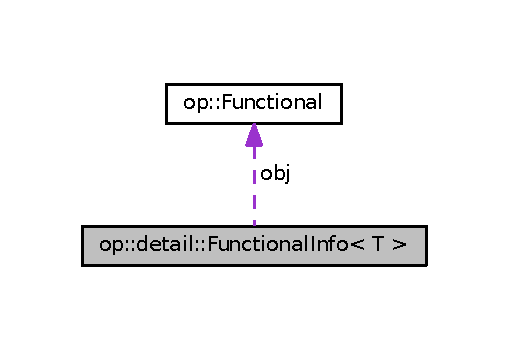
\includegraphics[width=244pt]{structop_1_1detail_1_1FunctionalInfo__coll__graph}
\end{center}
\end{figure}
\subsection*{Public Attributes}
\begin{DoxyCompactItemize}
\item 
\hypertarget{structop_1_1detail_1_1FunctionalInfo_a75b307e114fc03c879bb8fcfeeae83ad}{\hyperlink{classop_1_1Functional}{op\-::\-Functional} {\bfseries obj}}\label{structop_1_1detail_1_1FunctionalInfo_a75b307e114fc03c879bb8fcfeeae83ad}

\item 
\hypertarget{structop_1_1detail_1_1FunctionalInfo_a1cd58caba8132316014eb2367a11558d}{\hyperlink{classop_1_1NLopt}{op\-::\-N\-Lopt}$<$ T $>$ \& {\bfseries nlopt}}\label{structop_1_1detail_1_1FunctionalInfo_a1cd58caba8132316014eb2367a11558d}

\item 
\hypertarget{structop_1_1detail_1_1FunctionalInfo_a3af81392fd0b276d83f15fba073782bb}{int {\bfseries state}}\label{structop_1_1detail_1_1FunctionalInfo_a3af81392fd0b276d83f15fba073782bb}

\item 
\hypertarget{structop_1_1detail_1_1FunctionalInfo_a89df6f56725ac204f52f90ee260b36f6}{double {\bfseries constraint\-\_\-tol} = 0.}\label{structop_1_1detail_1_1FunctionalInfo_a89df6f56725ac204f52f90ee260b36f6}

\item 
\hypertarget{structop_1_1detail_1_1FunctionalInfo_a15287b9b16bd051c2cc6a4bc9fda8bf0}{double {\bfseries constraint\-\_\-val} = 0.}\label{structop_1_1detail_1_1FunctionalInfo_a15287b9b16bd051c2cc6a4bc9fda8bf0}

\item 
\hypertarget{structop_1_1detail_1_1FunctionalInfo_a8cdacd64fc88a319d3927008d523cd74}{bool {\bfseries lower\-\_\-bound} = false}\label{structop_1_1detail_1_1FunctionalInfo_a8cdacd64fc88a319d3927008d523cd74}

\end{DoxyCompactItemize}


\subsection{Detailed Description}
\subsubsection*{template$<$typename T$>$struct op\-::detail\-::\-Functional\-Info$<$ T $>$}

Container to pass objective and optimizer. 

Definition at line 21 of file nlopt\-\_\-op.\-hpp.



The documentation for this struct was generated from the following file\-:\begin{DoxyCompactItemize}
\item 
/usr/workspace/jekel1/\-Repos/op/src/nlopt\-\_\-op.\-hpp\end{DoxyCompactItemize}

\hypertarget{classop_1_1Go}{\section{op\-:\-:Go Class Reference}
\label{classop_1_1Go}\index{op\-::\-Go@{op\-::\-Go}}
}


{\ttfamily \#include $<$op.\-hpp$>$}

\subsection*{Public Member Functions}
\begin{DoxyCompactItemize}
\item 
\hypertarget{classop_1_1Go_a23151111fb0b066e589d75c0990a4a97}{\hyperlink{classop_1_1Go}{Go} \& \hyperlink{classop_1_1Go_a23151111fb0b066e589d75c0990a4a97}{on\-Preprocess} (const \hyperlink{namespaceop_aa384cc9d57783c0a83be03e0fcbab4f4}{Callback\-Fn} \&preprocess)}\label{classop_1_1Go_a23151111fb0b066e589d75c0990a4a97}

\begin{DoxyCompactList}\small\item\em Define preprocess action. \end{DoxyCompactList}\item 
\hypertarget{classop_1_1Go_a6eb0a46f6a2518065b4b9712f4c3ecea}{\hyperlink{classop_1_1Go}{Go} \& \hyperlink{classop_1_1Go_a6eb0a46f6a2518065b4b9712f4c3ecea}{on\-Go} (const \hyperlink{namespaceop_aa384cc9d57783c0a83be03e0fcbab4f4}{Callback\-Fn} \&go)}\label{classop_1_1Go_a6eb0a46f6a2518065b4b9712f4c3ecea}

\begin{DoxyCompactList}\small\item\em Define \hyperlink{classop_1_1Go}{Go} action. \end{DoxyCompactList}\item 
\hypertarget{classop_1_1Go_a78995ff12f276329f264e1415fd55bb4}{void {\bfseries operator()} ()}\label{classop_1_1Go_a78995ff12f276329f264e1415fd55bb4}

\end{DoxyCompactItemize}
\subsection*{Protected Attributes}
\begin{DoxyCompactItemize}
\item 
\hypertarget{classop_1_1Go_a60c9fda4b6b5c34ec77ee62a2149c072}{\hyperlink{namespaceop_aa384cc9d57783c0a83be03e0fcbab4f4}{Callback\-Fn} {\bfseries go\-\_\-}}\label{classop_1_1Go_a60c9fda4b6b5c34ec77ee62a2149c072}

\item 
\hypertarget{classop_1_1Go_ad0acc646b539b3fe33d8546e94fc86dc}{\hyperlink{namespaceop_aa384cc9d57783c0a83be03e0fcbab4f4}{Callback\-Fn} {\bfseries preprocess\-\_\-}}\label{classop_1_1Go_ad0acc646b539b3fe33d8546e94fc86dc}

\end{DoxyCompactItemize}


\subsection{Detailed Description}
\hyperlink{classop_1_1Go}{Go} Functor A functor to hold the optimization.\-Go() and .Preprocess() functions 

Definition at line 26 of file op.\-hpp.



The documentation for this class was generated from the following file\-:\begin{DoxyCompactItemize}
\item 
/usr/workspace/jekel1/\-Repos/op/src/op.\-hpp\end{DoxyCompactItemize}

\hypertarget{structop_1_1mpi_1_1detail_1_1has__data}{\section{op\-:\-:mpi\-:\-:detail\-:\-:has\-\_\-data$<$ T, S\-F\-I\-N\-A\-E $>$ Struct Template Reference}
\label{structop_1_1mpi_1_1detail_1_1has__data}\index{op\-::mpi\-::detail\-::has\-\_\-data$<$ T, S\-F\-I\-N\-A\-E $>$@{op\-::mpi\-::detail\-::has\-\_\-data$<$ T, S\-F\-I\-N\-A\-E $>$}}
}


Collaboration diagram for op\-:\-:mpi\-:\-:detail\-:\-:has\-\_\-data$<$ T, S\-F\-I\-N\-A\-E $>$\-:
\nopagebreak
\begin{figure}[H]
\begin{center}
\leavevmode
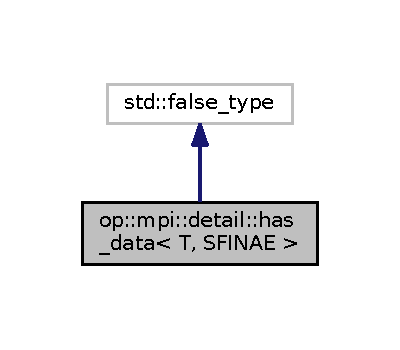
\includegraphics[width=192pt]{structop_1_1mpi_1_1detail_1_1has__data__coll__graph}
\end{center}
\end{figure}


\subsection{Detailed Description}
\subsubsection*{template$<$typename T, typename S\-F\-I\-N\-A\-E = void$>$struct op\-::mpi\-::detail\-::has\-\_\-data$<$ T, S\-F\-I\-N\-A\-E $>$}



Definition at line 32 of file op\-\_\-mpi.\-hpp.



The documentation for this struct was generated from the following file\-:\begin{DoxyCompactItemize}
\item 
/usr/workspace/jekel1/\-Repos/op/src/op\-\_\-mpi.\-hpp\end{DoxyCompactItemize}

\hypertarget{structop_1_1mpi_1_1detail_1_1has__data_3_01T_00_01std_1_1void__t_3_01decltype_07std_1_1declval_3524e889c05cc305ced759fca9c8b2769}{\section{op\-:\-:mpi\-:\-:detail\-:\-:has\-\_\-data$<$ T, std\-:\-:void\-\_\-t$<$ decltype(std\-:\-:declval$<$ T $>$().data())$>$ $>$ Struct Template Reference}
\label{structop_1_1mpi_1_1detail_1_1has__data_3_01T_00_01std_1_1void__t_3_01decltype_07std_1_1declval_3524e889c05cc305ced759fca9c8b2769}\index{op\-::mpi\-::detail\-::has\-\_\-data$<$ T, std\-::void\-\_\-t$<$ decltype(std\-::declval$<$ T $>$().\-data())$>$ $>$@{op\-::mpi\-::detail\-::has\-\_\-data$<$ T, std\-::void\-\_\-t$<$ decltype(std\-::declval$<$ T $>$().\-data())$>$ $>$}}
}


Collaboration diagram for op\-:\-:mpi\-:\-:detail\-:\-:has\-\_\-data$<$ T, std\-:\-:void\-\_\-t$<$ decltype(std\-:\-:declval$<$ T $>$().data())$>$ $>$\-:
\nopagebreak
\begin{figure}[H]
\begin{center}
\leavevmode
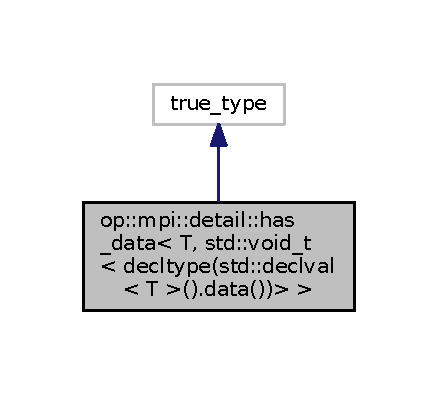
\includegraphics[width=210pt]{structop_1_1mpi_1_1detail_1_1has__data_3_01T_00_01std_1_1void__t_3_01decltype_07std_1_1declval_3de23e1dcf8c8ab7c2518859b32206103}
\end{center}
\end{figure}


\subsection{Detailed Description}
\subsubsection*{template$<$typename T$>$struct op\-::mpi\-::detail\-::has\-\_\-data$<$ T, std\-::void\-\_\-t$<$ decltype(std\-::declval$<$ T $>$().\-data())$>$ $>$}



Definition at line 36 of file op\-\_\-mpi.\-hpp.



The documentation for this struct was generated from the following file\-:\begin{DoxyCompactItemize}
\item 
/usr/workspace/jekel1/\-Repos/op/src/op\-\_\-mpi.\-hpp\end{DoxyCompactItemize}

\hypertarget{structop_1_1mpi_1_1detail_1_1has__size}{\section{op\-:\-:mpi\-:\-:detail\-:\-:has\-\_\-size$<$ T, S\-F\-I\-N\-A\-E $>$ Struct Template Reference}
\label{structop_1_1mpi_1_1detail_1_1has__size}\index{op\-::mpi\-::detail\-::has\-\_\-size$<$ T, S\-F\-I\-N\-A\-E $>$@{op\-::mpi\-::detail\-::has\-\_\-size$<$ T, S\-F\-I\-N\-A\-E $>$}}
}


Collaboration diagram for op\-:\-:mpi\-:\-:detail\-:\-:has\-\_\-size$<$ T, S\-F\-I\-N\-A\-E $>$\-:
\nopagebreak
\begin{figure}[H]
\begin{center}
\leavevmode
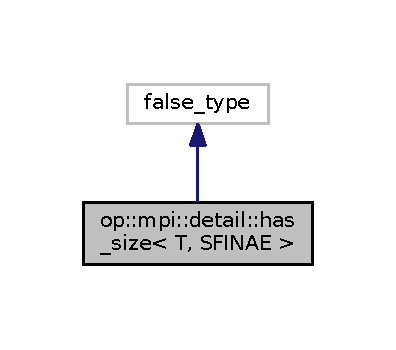
\includegraphics[width=190pt]{structop_1_1mpi_1_1detail_1_1has__size__coll__graph}
\end{center}
\end{figure}


\subsection{Detailed Description}
\subsubsection*{template$<$typename T, typename S\-F\-I\-N\-A\-E = void$>$struct op\-::mpi\-::detail\-::has\-\_\-size$<$ T, S\-F\-I\-N\-A\-E $>$}



Definition at line 40 of file op\-\_\-mpi.\-hpp.



The documentation for this struct was generated from the following file\-:\begin{DoxyCompactItemize}
\item 
/usr/workspace/jekel1/\-Repos/op/src/op\-\_\-mpi.\-hpp\end{DoxyCompactItemize}

\hypertarget{structop_1_1mpi_1_1detail_1_1has__size_3_01T_00_01std_1_1void__t_3_01decltype_07std_1_1declval_336d4e0461dc0efc09f20739ab7700530}{\section{op\-:\-:mpi\-:\-:detail\-:\-:has\-\_\-size$<$ T, std\-:\-:void\-\_\-t$<$ decltype(std\-:\-:declval$<$ T $>$().size())$>$ $>$ Struct Template Reference}
\label{structop_1_1mpi_1_1detail_1_1has__size_3_01T_00_01std_1_1void__t_3_01decltype_07std_1_1declval_336d4e0461dc0efc09f20739ab7700530}\index{op\-::mpi\-::detail\-::has\-\_\-size$<$ T, std\-::void\-\_\-t$<$ decltype(std\-::declval$<$ T $>$().\-size())$>$ $>$@{op\-::mpi\-::detail\-::has\-\_\-size$<$ T, std\-::void\-\_\-t$<$ decltype(std\-::declval$<$ T $>$().\-size())$>$ $>$}}
}


Collaboration diagram for op\-:\-:mpi\-:\-:detail\-:\-:has\-\_\-size$<$ T, std\-:\-:void\-\_\-t$<$ decltype(std\-:\-:declval$<$ T $>$().size())$>$ $>$\-:
\nopagebreak
\begin{figure}[H]
\begin{center}
\leavevmode
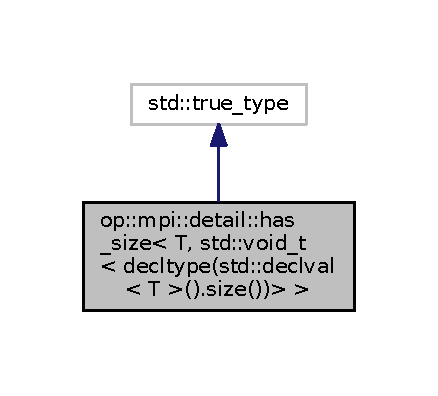
\includegraphics[width=210pt]{structop_1_1mpi_1_1detail_1_1has__size_3_01T_00_01std_1_1void__t_3_01decltype_07std_1_1declval_3b207867be39348695172c74d7e29575d}
\end{center}
\end{figure}


\subsection{Detailed Description}
\subsubsection*{template$<$typename T$>$struct op\-::mpi\-::detail\-::has\-\_\-size$<$ T, std\-::void\-\_\-t$<$ decltype(std\-::declval$<$ T $>$().\-size())$>$ $>$}



Definition at line 44 of file op\-\_\-mpi.\-hpp.



The documentation for this struct was generated from the following file\-:\begin{DoxyCompactItemize}
\item 
/usr/workspace/jekel1/\-Repos/op/src/op\-\_\-mpi.\-hpp\end{DoxyCompactItemize}

\hypertarget{structop_1_1mpi_1_1detail_1_1mpi__t}{\section{op\-:\-:mpi\-:\-:detail\-:\-:mpi\-\_\-t$<$ T $>$ Struct Template Reference}
\label{structop_1_1mpi_1_1detail_1_1mpi__t}\index{op\-::mpi\-::detail\-::mpi\-\_\-t$<$ T $>$@{op\-::mpi\-::detail\-::mpi\-\_\-t$<$ T $>$}}
}
\subsection*{Static Public Member Functions}
\begin{DoxyCompactItemize}
\item 
\hypertarget{structop_1_1mpi_1_1detail_1_1mpi__t_a0deba26f42782553da39503e7c0e741b}{static M\-P\-I\-\_\-\-Datatype {\bfseries type} ()}\label{structop_1_1mpi_1_1detail_1_1mpi__t_a0deba26f42782553da39503e7c0e741b}

\end{DoxyCompactItemize}


\subsection{Detailed Description}
\subsubsection*{template$<$typename T$>$struct op\-::mpi\-::detail\-::mpi\-\_\-t$<$ T $>$}



Definition at line 12 of file op\-\_\-mpi.\-hpp.



The documentation for this struct was generated from the following file\-:\begin{DoxyCompactItemize}
\item 
/usr/workspace/jekel1/\-Repos/op/src/op\-\_\-mpi.\-hpp\end{DoxyCompactItemize}

\hypertarget{structop_1_1mpi_1_1detail_1_1mpi__t_3_01double_01_4}{\section{op\-:\-:mpi\-:\-:detail\-:\-:mpi\-\_\-t$<$ double $>$ Struct Template Reference}
\label{structop_1_1mpi_1_1detail_1_1mpi__t_3_01double_01_4}\index{op\-::mpi\-::detail\-::mpi\-\_\-t$<$ double $>$@{op\-::mpi\-::detail\-::mpi\-\_\-t$<$ double $>$}}
}
\subsection*{Static Public Member Functions}
\begin{DoxyCompactItemize}
\item 
\hypertarget{structop_1_1mpi_1_1detail_1_1mpi__t_3_01double_01_4_ab700721841d0f23c664786c849725add}{static M\-P\-I\-\_\-\-Datatype {\bfseries type} ()}\label{structop_1_1mpi_1_1detail_1_1mpi__t_3_01double_01_4_ab700721841d0f23c664786c849725add}

\end{DoxyCompactItemize}


\subsection{Detailed Description}
\subsubsection*{template$<$$>$struct op\-::mpi\-::detail\-::mpi\-\_\-t$<$ double $>$}



Definition at line 17 of file op\-\_\-mpi.\-hpp.



The documentation for this struct was generated from the following file\-:\begin{DoxyCompactItemize}
\item 
/usr/workspace/jekel1/\-Repos/op/src/op\-\_\-mpi.\-hpp\end{DoxyCompactItemize}

\hypertarget{structop_1_1mpi_1_1detail_1_1mpi__t_3_01int_01_4}{\section{op\-:\-:mpi\-:\-:detail\-:\-:mpi\-\_\-t$<$ int $>$ Struct Template Reference}
\label{structop_1_1mpi_1_1detail_1_1mpi__t_3_01int_01_4}\index{op\-::mpi\-::detail\-::mpi\-\_\-t$<$ int $>$@{op\-::mpi\-::detail\-::mpi\-\_\-t$<$ int $>$}}
}
\subsection*{Static Public Member Functions}
\begin{DoxyCompactItemize}
\item 
\hypertarget{structop_1_1mpi_1_1detail_1_1mpi__t_3_01int_01_4_a76ea4ea9645edf67e08c164c92831b52}{static M\-P\-I\-\_\-\-Datatype {\bfseries type} ()}\label{structop_1_1mpi_1_1detail_1_1mpi__t_3_01int_01_4_a76ea4ea9645edf67e08c164c92831b52}

\end{DoxyCompactItemize}


\subsection{Detailed Description}
\subsubsection*{template$<$$>$struct op\-::mpi\-::detail\-::mpi\-\_\-t$<$ int $>$}



Definition at line 22 of file op\-\_\-mpi.\-hpp.



The documentation for this struct was generated from the following file\-:\begin{DoxyCompactItemize}
\item 
/usr/workspace/jekel1/\-Repos/op/src/op\-\_\-mpi.\-hpp\end{DoxyCompactItemize}

\hypertarget{structop_1_1mpi_1_1detail_1_1mpi__t_3_01unsigned_01long_01_4}{\section{op\-:\-:mpi\-:\-:detail\-:\-:mpi\-\_\-t$<$ unsigned long $>$ Struct Template Reference}
\label{structop_1_1mpi_1_1detail_1_1mpi__t_3_01unsigned_01long_01_4}\index{op\-::mpi\-::detail\-::mpi\-\_\-t$<$ unsigned long $>$@{op\-::mpi\-::detail\-::mpi\-\_\-t$<$ unsigned long $>$}}
}
\subsection*{Static Public Member Functions}
\begin{DoxyCompactItemize}
\item 
\hypertarget{structop_1_1mpi_1_1detail_1_1mpi__t_3_01unsigned_01long_01_4_a8d964864aa50ef5831788d26be3bb412}{static M\-P\-I\-\_\-\-Datatype {\bfseries type} ()}\label{structop_1_1mpi_1_1detail_1_1mpi__t_3_01unsigned_01long_01_4_a8d964864aa50ef5831788d26be3bb412}

\end{DoxyCompactItemize}


\subsection{Detailed Description}
\subsubsection*{template$<$$>$struct op\-::mpi\-::detail\-::mpi\-\_\-t$<$ unsigned long $>$}



Definition at line 27 of file op\-\_\-mpi.\-hpp.



The documentation for this struct was generated from the following file\-:\begin{DoxyCompactItemize}
\item 
/usr/workspace/jekel1/\-Repos/op/src/op\-\_\-mpi.\-hpp\end{DoxyCompactItemize}

\hypertarget{classop_1_1NLopt}{\section{op\-:\-:N\-Lopt$<$ T $>$ Class Template Reference}
\label{classop_1_1NLopt}\index{op\-::\-N\-Lopt$<$ T $>$@{op\-::\-N\-Lopt$<$ T $>$}}
}


A op\-::optimizer implementation for \hyperlink{classop_1_1NLopt}{N\-Lopt}.  




{\ttfamily \#include $<$nlopt\-\_\-op.\-hpp$>$}



Collaboration diagram for op\-:\-:N\-Lopt$<$ T $>$\-:
\nopagebreak
\begin{figure}[H]
\begin{center}
\leavevmode
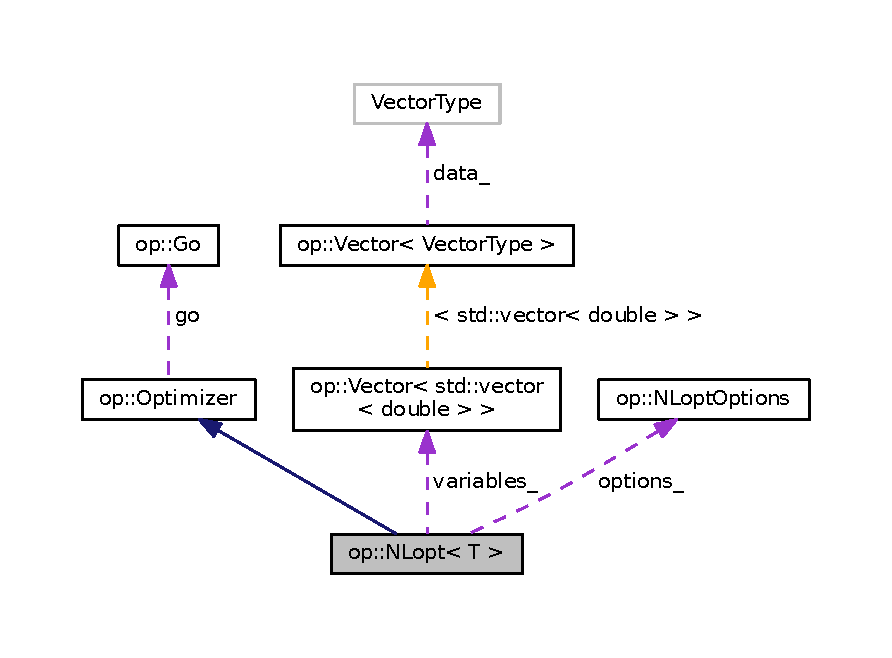
\includegraphics[width=350pt]{classop_1_1NLopt__coll__graph}
\end{center}
\end{figure}
\subsection*{Public Member Functions}
\begin{DoxyCompactItemize}
\item 
\hypertarget{classop_1_1NLopt_a1ed2908f747c6506ac7d28fb92d01ede}{\hyperlink{classop_1_1NLopt_a1ed2908f747c6506ac7d28fb92d01ede}{N\-Lopt} (\hyperlink{classop_1_1Vector}{op\-::\-Vector}$<$ std\-::vector$<$ double $>$$>$ \&variables, \hyperlink{structop_1_1NLoptOptions}{N\-Lopt\-Options} \&o, std\-::optional$<$ M\-P\-I\-\_\-\-Comm $>$ comm=\{\}, std\-::optional$<$ \hyperlink{structop_1_1utility_1_1CommPattern}{op\-::utility\-::\-Comm\-Pattern}$<$ T $>$$>$ comm\-\_\-pattern\-\_\-info=\{\})}\label{classop_1_1NLopt_a1ed2908f747c6506ac7d28fb92d01ede}

\begin{DoxyCompactList}\small\item\em Constructor for our optimizer. \end{DoxyCompactList}\item 
\hypertarget{classop_1_1NLopt_a2ee351c67324faded262583c27dabe00}{{\bfseries num\-\_\-local\-\_\-owned\-\_\-variables\-\_\-} (0)}\label{classop_1_1NLopt_a2ee351c67324faded262583c27dabe00}

\item 
void \hyperlink{classop_1_1NLopt_afe2f2eca4b0fd4b8d2aa0e819f8bd83f}{set\-Objective} (\hyperlink{classop_1_1Functional}{op\-::\-Functional} \&o) override
\begin{DoxyCompactList}\small\item\em Sets the optimization objective. \end{DoxyCompactList}\item 
void \hyperlink{classop_1_1NLopt_aad04273dde9c66444ed727928fcc6197}{add\-Constraint} (\hyperlink{classop_1_1Functional}{op\-::\-Functional} \&o) override
\begin{DoxyCompactList}\small\item\em Adds a constraint for the optimization problem. \end{DoxyCompactList}\item 
bool \hyperlink{classop_1_1NLopt_ad92c30719e3cc720ebefccedd591e543}{variables\-\_\-changed} (const std\-::vector$<$ double $>$ \&x)
\begin{DoxyCompactList}\small\item\em Method to see if variables changed, if they have set new x. \end{DoxyCompactList}\item 
\hypertarget{classop_1_1NLopt_a5c54d30b88b4de8b19774cd3fb12f482}{bool \hyperlink{classop_1_1NLopt_a5c54d30b88b4de8b19774cd3fb12f482}{is\-Advanced} ()}\label{classop_1_1NLopt_a5c54d30b88b4de8b19774cd3fb12f482}

\begin{DoxyCompactList}\small\item\em returns whether \hyperlink{classop_1_1NLopt}{N\-Lopt} is in \char`\"{}advanced\char`\"{} mode or not \end{DoxyCompactList}\item 
\hypertarget{classop_1_1NLopt_a94355fcd880ccac99e0056c2950289fa}{auto \hyperlink{classop_1_1NLopt_a94355fcd880ccac99e0056c2950289fa}{generate\-Reduced\-Local\-Gradient\-Function} (std\-::function$<$ std\-::vector$<$ double $>$(const std\-::vector$<$ double $>$ \&)$>$ local\-\_\-grad\-\_\-func, std\-::function$<$ double(const std\-::vector$<$ double $>$ \&)$>$ local\-\_\-reduce\-\_\-func)}\label{classop_1_1NLopt_a94355fcd880ccac99e0056c2950289fa}

\begin{DoxyCompactList}\small\item\em generates reduced local gradient using comm\-\_\-pattern\-\_\- \end{DoxyCompactList}\end{DoxyCompactItemize}
\subsection*{Protected Attributes}
\begin{DoxyCompactItemize}
\item 
\hypertarget{classop_1_1NLopt_a1d365f27aac2aa7f534759f3d8a29543}{M\-P\-I\-\_\-\-Comm {\bfseries comm\-\_\-}}\label{classop_1_1NLopt_a1d365f27aac2aa7f534759f3d8a29543}

\item 
\hypertarget{classop_1_1NLopt_a7045da58c5ed2236a183ed9a6e68b1ff}{std\-::vector$<$ double $>$ {\bfseries global\-\_\-variables\-\_\-}}\label{classop_1_1NLopt_a7045da58c5ed2236a183ed9a6e68b1ff}

\item 
\hypertarget{classop_1_1NLopt_aba440212096236a4dc975e0b75dcfc08}{\hyperlink{classop_1_1Vector}{op\-::\-Vector}$<$ std\-::vector\\*
$<$ double $>$ $>$ \& {\bfseries variables\-\_\-}}\label{classop_1_1NLopt_aba440212096236a4dc975e0b75dcfc08}

\item 
\hypertarget{classop_1_1NLopt_a2591bf6066bb893841376cd98de05410}{std\-::unique\-\_\-ptr$<$ nlopt\-::opt $>$ {\bfseries nlopt\-\_\-}}\label{classop_1_1NLopt_a2591bf6066bb893841376cd98de05410}

\item 
\hypertarget{classop_1_1NLopt_a89cfca2c991cb9a0fcb188a7a2fb7515}{\hyperlink{structop_1_1NLoptOptions}{N\-Lopt\-Options} \& {\bfseries options\-\_\-}}\label{classop_1_1NLopt_a89cfca2c991cb9a0fcb188a7a2fb7515}

\item 
\hypertarget{classop_1_1NLopt_a3f57509a1e31358e7557074efd3c6085}{std\-::vector$<$ double $>$ {\bfseries previous\-\_\-variables\-\_\-}}\label{classop_1_1NLopt_a3f57509a1e31358e7557074efd3c6085}

\item 
\hypertarget{classop_1_1NLopt_a16d7a19a7c9b1d78f06f7f1090277e5d}{std\-::vector\\*
$<$ \hyperlink{structop_1_1detail_1_1FunctionalInfo}{detail\-::\-Functional\-Info}$<$ T $>$ $>$ {\bfseries obj\-\_\-info\-\_\-}}\label{classop_1_1NLopt_a16d7a19a7c9b1d78f06f7f1090277e5d}

\item 
\hypertarget{classop_1_1NLopt_aded0811d6cc7ab5792396c7bdf7f8ef1}{std\-::vector\\*
$<$ \hyperlink{structop_1_1detail_1_1FunctionalInfo}{detail\-::\-Functional\-Info}$<$ T $>$ $>$ {\bfseries constraints\-\_\-info\-\_\-}}\label{classop_1_1NLopt_aded0811d6cc7ab5792396c7bdf7f8ef1}

\item 
\hypertarget{classop_1_1NLopt_ad38e598bdc610c3dcc6c4611cf1333e1}{std\-::vector$<$ int $>$ {\bfseries owned\-\_\-variables\-\_\-per\-\_\-rank\-\_\-}}\label{classop_1_1NLopt_ad38e598bdc610c3dcc6c4611cf1333e1}

\item 
\hypertarget{classop_1_1NLopt_a1376429626ecfd58dea3ea99e0b258c9}{std\-::vector$<$ int $>$ {\bfseries owned\-\_\-offsets\-\_\-}}\label{classop_1_1NLopt_a1376429626ecfd58dea3ea99e0b258c9}

\item 
\hypertarget{classop_1_1NLopt_a6595246d545758fe572dc1f786155dd3}{std\-::optional\\*
$<$ \hyperlink{structop_1_1utility_1_1CommPattern}{utility\-::\-Comm\-Pattern}$<$ T $>$ $>$ {\bfseries comm\-\_\-pattern\-\_\-}}\label{classop_1_1NLopt_a6595246d545758fe572dc1f786155dd3}

\item 
\hypertarget{classop_1_1NLopt_a25e6ed69156a0554a3d705d263bcf46a}{std\-::optional\\*
$<$ std\-::unordered\-\_\-map$<$ typename \\*
T\-::value\-\_\-type, T $>$ $>$ {\bfseries global\-\_\-reduced\-\_\-map\-\_\-to\-\_\-local\-\_\-}}\label{classop_1_1NLopt_a25e6ed69156a0554a3d705d263bcf46a}

\item 
\hypertarget{classop_1_1NLopt_a8d375f203c2f7a4786d2ee3d17be4ec0}{std\-::size\-\_\-t {\bfseries num\-\_\-local\-\_\-owned\-\_\-variables\-\_\-}}\label{classop_1_1NLopt_a8d375f203c2f7a4786d2ee3d17be4ec0}

\item 
\hypertarget{classop_1_1NLopt_a77c36eaeb9124a0886f8224735684433}{int {\bfseries root\-\_\-rank\-\_\-} = 0}\label{classop_1_1NLopt_a77c36eaeb9124a0886f8224735684433}

\item 
\hypertarget{classop_1_1NLopt_a5441290e7186be77f81626bb31ba8fa2}{std\-::unique\-\_\-ptr$<$ \hyperlink{classop_1_1WaitLoop}{Wait\-Loop} $>$ {\bfseries waitloop\-\_\-}}\label{classop_1_1NLopt_a5441290e7186be77f81626bb31ba8fa2}

\end{DoxyCompactItemize}
\subsection*{Friends}
\begin{DoxyCompactItemize}
\item 
double \hyperlink{classop_1_1NLopt_a29d5ab6d03460755684ce25f13da7ae5}{N\-Lopt\-Functional} (const std\-::vector$<$ double $>$ \&x, std\-::vector$<$ double $>$ \&grad, void $\ast$objective\-\_\-and\-\_\-optimizer)
\begin{DoxyCompactList}\small\item\em Takes in a \hyperlink{classop_1_1Functional}{op\-::\-Functional} and computes the objective function and it's gradient as a nlopt function. \end{DoxyCompactList}\end{DoxyCompactItemize}
\subsection*{Additional Inherited Members}


\subsection{Detailed Description}
\subsubsection*{template$<$typename T$>$class op\-::\-N\-Lopt$<$ T $>$}

A op\-::optimizer implementation for \hyperlink{classop_1_1NLopt}{N\-Lopt}. 

Definition at line 15 of file nlopt\-\_\-op.\-hpp.



\subsection{Member Function Documentation}
\hypertarget{classop_1_1NLopt_aad04273dde9c66444ed727928fcc6197}{\index{op\-::\-N\-Lopt@{op\-::\-N\-Lopt}!add\-Constraint@{add\-Constraint}}
\index{add\-Constraint@{add\-Constraint}!op::NLopt@{op\-::\-N\-Lopt}}
\subsubsection[{add\-Constraint}]{\setlength{\rightskip}{0pt plus 5cm}template$<$typename T $>$ void {\bf op\-::\-N\-Lopt}$<$ T $>$\-::add\-Constraint (
\begin{DoxyParamCaption}
\item[{{\bf op\-::\-Functional} \&}]{}
\end{DoxyParamCaption}
)\hspace{0.3cm}{\ttfamily [inline]}, {\ttfamily [override]}, {\ttfamily [virtual]}}}\label{classop_1_1NLopt_aad04273dde9c66444ed727928fcc6197}


Adds a constraint for the optimization problem. 


\begin{DoxyParams}[1]{Parameters}
\mbox{\tt in}  & {\em o} & Constraint \hyperlink{classop_1_1Functional}{Functional} \\
\hline
\end{DoxyParams}


Reimplemented from \hyperlink{classop_1_1Optimizer_ae5a8f5522cb39299687127115a904854}{op\-::\-Optimizer}.



Definition at line 305 of file nlopt\-\_\-op.\-hpp.

\hypertarget{classop_1_1NLopt_afe2f2eca4b0fd4b8d2aa0e819f8bd83f}{\index{op\-::\-N\-Lopt@{op\-::\-N\-Lopt}!set\-Objective@{set\-Objective}}
\index{set\-Objective@{set\-Objective}!op::NLopt@{op\-::\-N\-Lopt}}
\subsubsection[{set\-Objective}]{\setlength{\rightskip}{0pt plus 5cm}template$<$typename T $>$ void {\bf op\-::\-N\-Lopt}$<$ T $>$\-::set\-Objective (
\begin{DoxyParamCaption}
\item[{{\bf op\-::\-Functional} \&}]{o}
\end{DoxyParamCaption}
)\hspace{0.3cm}{\ttfamily [inline]}, {\ttfamily [override]}, {\ttfamily [virtual]}}}\label{classop_1_1NLopt_afe2f2eca4b0fd4b8d2aa0e819f8bd83f}


Sets the optimization objective. 


\begin{DoxyParams}[1]{Parameters}
\mbox{\tt in}  & {\em o} & Objective \hyperlink{classop_1_1Functional}{Functional} \\
\hline
\end{DoxyParams}


Implements \hyperlink{classop_1_1Optimizer_aace5e17d5ee0c38cd6f411d21dc2c3b0}{op\-::\-Optimizer}.



Definition at line 298 of file nlopt\-\_\-op.\-hpp.

\hypertarget{classop_1_1NLopt_ad92c30719e3cc720ebefccedd591e543}{\index{op\-::\-N\-Lopt@{op\-::\-N\-Lopt}!variables\-\_\-changed@{variables\-\_\-changed}}
\index{variables\-\_\-changed@{variables\-\_\-changed}!op::NLopt@{op\-::\-N\-Lopt}}
\subsubsection[{variables\-\_\-changed}]{\setlength{\rightskip}{0pt plus 5cm}template$<$typename T $>$ bool {\bf op\-::\-N\-Lopt}$<$ T $>$\-::variables\-\_\-changed (
\begin{DoxyParamCaption}
\item[{const std\-::vector$<$ double $>$ \&}]{x}
\end{DoxyParamCaption}
)\hspace{0.3cm}{\ttfamily [inline]}}}\label{classop_1_1NLopt_ad92c30719e3cc720ebefccedd591e543}


Method to see if variables changed, if they have set new x. 


\begin{DoxyParams}[1]{Parameters}
\mbox{\tt in}  & {\em x} & \\
\hline
\end{DoxyParams}


Definition at line 331 of file nlopt\-\_\-op.\-hpp.



\subsection{Friends And Related Function Documentation}
\hypertarget{classop_1_1NLopt_a29d5ab6d03460755684ce25f13da7ae5}{\index{op\-::\-N\-Lopt@{op\-::\-N\-Lopt}!N\-Lopt\-Functional@{N\-Lopt\-Functional}}
\index{N\-Lopt\-Functional@{N\-Lopt\-Functional}!op::NLopt@{op\-::\-N\-Lopt}}
\subsubsection[{N\-Lopt\-Functional}]{\setlength{\rightskip}{0pt plus 5cm}template$<$typename T $>$ double N\-Lopt\-Functional (
\begin{DoxyParamCaption}
\item[{const std\-::vector$<$ double $>$ \&}]{x, }
\item[{std\-::vector$<$ double $>$ \&}]{grad, }
\item[{void $\ast$}]{objective\-\_\-and\-\_\-optimizer}
\end{DoxyParamCaption}
)\hspace{0.3cm}{\ttfamily [friend]}}}\label{classop_1_1NLopt_a29d5ab6d03460755684ce25f13da7ae5}


Takes in a \hyperlink{classop_1_1Functional}{op\-::\-Functional} and computes the objective function and it's gradient as a nlopt function. 

Has the same signature as nlopt\-::function so we can convert any \hyperlink{classop_1_1Functional}{op\-::\-Functional} into a nlopt\-::function 
\begin{DoxyParams}[1]{Parameters}
\mbox{\tt in}  & {\em x} & the optimization variables (on rank = 0 this is the actual global optimization variables, on other ranks it is the local-\/view of variables.\-data()) \\
\hline
\mbox{\tt in}  & {\em grad} & the result of the gradient of the function w.\-r.\-t. x (on rank 0, this is the global gradient eval, on other ranks it is the owned-\/local gradient) \\
\hline
\mbox{\tt in}  & {\em objective} & Get Functional\-Info into this call \\
\hline
\end{DoxyParams}
for constraints g $>$= lower\-\_\-bound, they need to be rewritten as -\/(g -\/ lower\-\_\-bound) $<$= 0

for constraints g $<$= upper\-\_\-bound, they need to be rewritten as g -\/ upper\-\_\-bound $<$ = 0

The documentation for this class was generated from the following file\-:\begin{DoxyCompactItemize}
\item 
/usr/workspace/jekel1/\-Repos/op/src/nlopt\-\_\-op.\-hpp\end{DoxyCompactItemize}

\hypertarget{structop_1_1NLoptOptions}{\section{op\-:\-:N\-Lopt\-Options Struct Reference}
\label{structop_1_1NLoptOptions}\index{op\-::\-N\-Lopt\-Options@{op\-::\-N\-Lopt\-Options}}
}


Options specific for nlopt. They are made to look like ipopt's interface.  




{\ttfamily \#include $<$nlopt\-\_\-op.\-hpp$>$}

\subsection*{Public Attributes}
\begin{DoxyCompactItemize}
\item 
\hypertarget{structop_1_1NLoptOptions_a0f28c9240152bce6d9fb75af85bd4d3e}{std\-::unordered\-\_\-map\\*
$<$ std\-::string, int $>$ {\bfseries Int}}\label{structop_1_1NLoptOptions_a0f28c9240152bce6d9fb75af85bd4d3e}

\item 
\hypertarget{structop_1_1NLoptOptions_af38f09e645969cab75a4c88117c29b4a}{std\-::unordered\-\_\-map\\*
$<$ std\-::string, double $>$ {\bfseries Double}}\label{structop_1_1NLoptOptions_af38f09e645969cab75a4c88117c29b4a}

\item 
\hypertarget{structop_1_1NLoptOptions_a7cecdd007ba62f59ad5b46b84baf1d28}{std\-::unordered\-\_\-map\\*
$<$ std\-::string, std\-::string $>$ {\bfseries String}}\label{structop_1_1NLoptOptions_a7cecdd007ba62f59ad5b46b84baf1d28}

\item 
\hypertarget{structop_1_1NLoptOptions_ad914b48412cb1ec19f6d8b571917626b}{nlopt\-::algorithm {\bfseries algorithm} = nlopt\-::\-L\-D\-\_\-\-M\-M\-A}\label{structop_1_1NLoptOptions_ad914b48412cb1ec19f6d8b571917626b}

\end{DoxyCompactItemize}


\subsection{Detailed Description}
Options specific for nlopt. They are made to look like ipopt's interface. 

Definition at line 55 of file nlopt\-\_\-op.\-hpp.



The documentation for this struct was generated from the following file\-:\begin{DoxyCompactItemize}
\item 
/usr/workspace/jekel1/\-Repos/op/src/nlopt\-\_\-op.\-hpp\end{DoxyCompactItemize}

\hypertarget{classop_1_1Optimizer}{\section{op\-:\-:Optimizer Class Reference}
\label{classop_1_1Optimizer}\index{op\-::\-Optimizer@{op\-::\-Optimizer}}
}


Abstracted \hyperlink{classop_1_1Optimizer}{Optimizer} implementation.  




{\ttfamily \#include $<$op.\-hpp$>$}



Collaboration diagram for op\-:\-:Optimizer\-:
\nopagebreak
\begin{figure}[H]
\begin{center}
\leavevmode
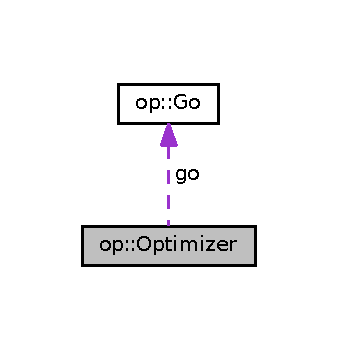
\includegraphics[width=162pt]{classop_1_1Optimizer__coll__graph}
\end{center}
\end{figure}
\subsection*{Public Member Functions}
\begin{DoxyCompactItemize}
\item 
\hypertarget{classop_1_1Optimizer_a49e7cc7189b76c4e87bed1431f76971b}{\hyperlink{classop_1_1Optimizer_a49e7cc7189b76c4e87bed1431f76971b}{Optimizer} ()}\label{classop_1_1Optimizer_a49e7cc7189b76c4e87bed1431f76971b}

\begin{DoxyCompactList}\small\item\em Ctor has deferred initialization. \end{DoxyCompactList}\item 
\hypertarget{classop_1_1Optimizer_adbb150d1945b1dd1826be17db7bf04a4}{{\bfseries iterate} (\mbox{[}$\,$\mbox{]}()\{\})}\label{classop_1_1Optimizer_adbb150d1945b1dd1826be17db7bf04a4}

\item 
\hypertarget{classop_1_1Optimizer_afe5f788cd6b7d4fbe841259d288de856}{{\bfseries save} (\mbox{[}$\,$\mbox{]}()\{\})}\label{classop_1_1Optimizer_afe5f788cd6b7d4fbe841259d288de856}

\item 
\hypertarget{classop_1_1Optimizer_a8221b2206aaf7cfea9edecb8bcf80acc}{{\bfseries final\-\_\-obj} (std\-::numeric\-\_\-limits$<$ double $>$\-::max())}\label{classop_1_1Optimizer_a8221b2206aaf7cfea9edecb8bcf80acc}

\item 
virtual void \hyperlink{classop_1_1Optimizer_aace5e17d5ee0c38cd6f411d21dc2c3b0}{set\-Objective} (\hyperlink{classop_1_1Functional}{Functional} \&o)=0
\begin{DoxyCompactList}\small\item\em Sets the optimization objective. \end{DoxyCompactList}\item 
virtual void \hyperlink{classop_1_1Optimizer_ae5a8f5522cb39299687127115a904854}{add\-Constraint} (\hyperlink{classop_1_1Functional}{Functional} \&)
\begin{DoxyCompactList}\small\item\em Adds a constraint for the optimization problem. \end{DoxyCompactList}\item 
\hypertarget{classop_1_1Optimizer_a85dc4b913a2a68be6b163ca65397798f}{void \hyperlink{classop_1_1Optimizer_a85dc4b913a2a68be6b163ca65397798f}{Go} ()}\label{classop_1_1Optimizer_a85dc4b913a2a68be6b163ca65397798f}

\begin{DoxyCompactList}\small\item\em Start the optimization. \end{DoxyCompactList}\item 
\hypertarget{classop_1_1Optimizer_a5da854fdf2fcffdd23306eb217bfda72}{void \hyperlink{classop_1_1Optimizer_a5da854fdf2fcffdd23306eb217bfda72}{Updated\-Variable\-Callback} ()}\label{classop_1_1Optimizer_a5da854fdf2fcffdd23306eb217bfda72}

\begin{DoxyCompactList}\small\item\em What to do when the variables are updated. \end{DoxyCompactList}\item 
\hypertarget{classop_1_1Optimizer_a01eaee3352a45aed066cc20a0bb350fa}{virtual double \hyperlink{classop_1_1Optimizer_a01eaee3352a45aed066cc20a0bb350fa}{Solution} ()}\label{classop_1_1Optimizer_a01eaee3352a45aed066cc20a0bb350fa}

\begin{DoxyCompactList}\small\item\em What to do when the solution is found. Return the objetive. \end{DoxyCompactList}\item 
\hypertarget{classop_1_1Optimizer_ad0fd6a7a4d8e9ca7fa4bc19e4324398a}{void \hyperlink{classop_1_1Optimizer_ad0fd6a7a4d8e9ca7fa4bc19e4324398a}{Iteration} ()}\label{classop_1_1Optimizer_ad0fd6a7a4d8e9ca7fa4bc19e4324398a}

\begin{DoxyCompactList}\small\item\em What to do at the end of an optimization iteration. \end{DoxyCompactList}\item 
\hypertarget{classop_1_1Optimizer_a0895f1f34e3ed2be29c353b8c3af81c3}{void \hyperlink{classop_1_1Optimizer_a0895f1f34e3ed2be29c353b8c3af81c3}{Save\-State} ()}\label{classop_1_1Optimizer_a0895f1f34e3ed2be29c353b8c3af81c3}

\begin{DoxyCompactList}\small\item\em Saves the state of the optimizer. \end{DoxyCompactList}\item 
\hypertarget{classop_1_1Optimizer_a64e00a7291d7b7e4c394c2278f1b406b}{virtual \hyperlink{classop_1_1Optimizer_a64e00a7291d7b7e4c394c2278f1b406b}{$\sim$\-Optimizer} ()=default}\label{classop_1_1Optimizer_a64e00a7291d7b7e4c394c2278f1b406b}

\begin{DoxyCompactList}\small\item\em Destructor. \end{DoxyCompactList}\end{DoxyCompactItemize}
\subsection*{Public Attributes}
\begin{DoxyCompactItemize}
\item 
\hypertarget{classop_1_1Optimizer_a2ce0f9e31b50befa3b747c45256a16e7}{\hyperlink{classop_1_1Go}{op\-::\-Go} \hyperlink{classop_1_1Optimizer_a2ce0f9e31b50befa3b747c45256a16e7}{go}}\label{classop_1_1Optimizer_a2ce0f9e31b50befa3b747c45256a16e7}

\begin{DoxyCompactList}\small\item\em \hyperlink{classop_1_1Go}{Go} function to start optimization. \end{DoxyCompactList}\item 
\hypertarget{classop_1_1Optimizer_a85c796202238fea34870e33f5c90ab1e}{\hyperlink{namespaceop_aa384cc9d57783c0a83be03e0fcbab4f4}{Callback\-Fn} \hyperlink{classop_1_1Optimizer_a85c796202238fea34870e33f5c90ab1e}{update}}\label{classop_1_1Optimizer_a85c796202238fea34870e33f5c90ab1e}

\begin{DoxyCompactList}\small\item\em Update callback to compute before function calculations. \end{DoxyCompactList}\item 
\hypertarget{classop_1_1Optimizer_a5dd4f175a15542dd57f442e093e30515}{\hyperlink{namespaceop_aa384cc9d57783c0a83be03e0fcbab4f4}{Callback\-Fn} \hyperlink{classop_1_1Optimizer_a5dd4f175a15542dd57f442e093e30515}{iterate}}\label{classop_1_1Optimizer_a5dd4f175a15542dd57f442e093e30515}

\begin{DoxyCompactList}\small\item\em iterate callback to compute before \end{DoxyCompactList}\item 
\hypertarget{classop_1_1Optimizer_a3f7887be306784dc329c24e43b14f252}{\hyperlink{namespaceop_aa384cc9d57783c0a83be03e0fcbab4f4}{Callback\-Fn} \hyperlink{classop_1_1Optimizer_a3f7887be306784dc329c24e43b14f252}{save}}\label{classop_1_1Optimizer_a3f7887be306784dc329c24e43b14f252}

\begin{DoxyCompactList}\small\item\em callback for saving current optimizer state \end{DoxyCompactList}\item 
\hypertarget{classop_1_1Optimizer_a74ab5895a6f2b74f155f19bd7a1e6f5a}{double \hyperlink{classop_1_1Optimizer_a74ab5895a6f2b74f155f19bd7a1e6f5a}{final\-\_\-obj}}\label{classop_1_1Optimizer_a74ab5895a6f2b74f155f19bd7a1e6f5a}

\begin{DoxyCompactList}\small\item\em final objective value \end{DoxyCompactList}\end{DoxyCompactItemize}


\subsection{Detailed Description}
Abstracted \hyperlink{classop_1_1Optimizer}{Optimizer} implementation. 

Definition at line 165 of file op.\-hpp.



\subsection{Member Function Documentation}
\hypertarget{classop_1_1Optimizer_ae5a8f5522cb39299687127115a904854}{\index{op\-::\-Optimizer@{op\-::\-Optimizer}!add\-Constraint@{add\-Constraint}}
\index{add\-Constraint@{add\-Constraint}!op::Optimizer@{op\-::\-Optimizer}}
\subsubsection[{add\-Constraint}]{\setlength{\rightskip}{0pt plus 5cm}virtual void op\-::\-Optimizer\-::add\-Constraint (
\begin{DoxyParamCaption}
\item[{{\bf Functional} \&}]{}
\end{DoxyParamCaption}
)\hspace{0.3cm}{\ttfamily [inline]}, {\ttfamily [virtual]}}}\label{classop_1_1Optimizer_ae5a8f5522cb39299687127115a904854}


Adds a constraint for the optimization problem. 


\begin{DoxyParams}[1]{Parameters}
\mbox{\tt in}  & {\em o} & Constraint \hyperlink{classop_1_1Functional}{Functional} \\
\hline
\end{DoxyParams}


Reimplemented in \hyperlink{classop_1_1NLopt_aad04273dde9c66444ed727928fcc6197}{op\-::\-N\-Lopt$<$ T $>$}.



Definition at line 186 of file op.\-hpp.

\hypertarget{classop_1_1Optimizer_aace5e17d5ee0c38cd6f411d21dc2c3b0}{\index{op\-::\-Optimizer@{op\-::\-Optimizer}!set\-Objective@{set\-Objective}}
\index{set\-Objective@{set\-Objective}!op::Optimizer@{op\-::\-Optimizer}}
\subsubsection[{set\-Objective}]{\setlength{\rightskip}{0pt plus 5cm}virtual void op\-::\-Optimizer\-::set\-Objective (
\begin{DoxyParamCaption}
\item[{{\bf Functional} \&}]{o}
\end{DoxyParamCaption}
)\hspace{0.3cm}{\ttfamily [pure virtual]}}}\label{classop_1_1Optimizer_aace5e17d5ee0c38cd6f411d21dc2c3b0}


Sets the optimization objective. 


\begin{DoxyParams}[1]{Parameters}
\mbox{\tt in}  & {\em o} & Objective \hyperlink{classop_1_1Functional}{Functional} \\
\hline
\end{DoxyParams}


Implemented in \hyperlink{classop_1_1NLopt_afe2f2eca4b0fd4b8d2aa0e819f8bd83f}{op\-::\-N\-Lopt$<$ T $>$}, and \hyperlink{classTestOptimizer_acf4e70d78cbbb9dd44e002575d4477f7}{Test\-Optimizer}.



The documentation for this class was generated from the following file\-:\begin{DoxyCompactItemize}
\item 
/usr/workspace/jekel1/\-Repos/op/src/op.\-hpp\end{DoxyCompactItemize}

\hypertarget{structop_1_1utility_1_1RankCommunication}{\section{op\-:\-:utility\-:\-:Rank\-Communication$<$ T $>$ Struct Template Reference}
\label{structop_1_1utility_1_1RankCommunication}\index{op\-::utility\-::\-Rank\-Communication$<$ T $>$@{op\-::utility\-::\-Rank\-Communication$<$ T $>$}}
}


Holds communication information to and from rank.  




{\ttfamily \#include $<$op\-\_\-utility.\-hpp$>$}

\subsection*{Public Types}
\begin{DoxyCompactItemize}
\item 
\hypertarget{structop_1_1utility_1_1RankCommunication_ac666b7c8853fb4ddae567e3f02b11812}{using {\bfseries value\-\_\-type} = T}\label{structop_1_1utility_1_1RankCommunication_ac666b7c8853fb4ddae567e3f02b11812}

\item 
\hypertarget{structop_1_1utility_1_1RankCommunication_a4eabbd32df0d34c84fc7f20f4f50029e}{using {\bfseries key\-\_\-type} = int}\label{structop_1_1utility_1_1RankCommunication_a4eabbd32df0d34c84fc7f20f4f50029e}

\end{DoxyCompactItemize}
\subsection*{Public Attributes}
\begin{DoxyCompactItemize}
\item 
\hypertarget{structop_1_1utility_1_1RankCommunication_a381599dde9ebbcb9beae742d287e4977}{std\-::unordered\-\_\-map$<$ int, T $>$ {\bfseries recv}}\label{structop_1_1utility_1_1RankCommunication_a381599dde9ebbcb9beae742d287e4977}

\item 
\hypertarget{structop_1_1utility_1_1RankCommunication_a9108f92d0dda9d382d5b91a14ac7fea8}{std\-::unordered\-\_\-map$<$ int, T $>$ {\bfseries send}}\label{structop_1_1utility_1_1RankCommunication_a9108f92d0dda9d382d5b91a14ac7fea8}

\end{DoxyCompactItemize}


\subsection{Detailed Description}
\subsubsection*{template$<$typename T$>$struct op\-::utility\-::\-Rank\-Communication$<$ T $>$}

Holds communication information to and from rank. 

Maps index information recieved and sent from a rank. Indices recieved for a given rank record contributions in terms of local rank indices. e.\-g. rank 1\-: \{1, 4, 5\} means that rank 1 contributes to local variable index 1, 4, and 5. 

Definition at line 18 of file op\-\_\-utility.\-hpp.



The documentation for this struct was generated from the following file\-:\begin{DoxyCompactItemize}
\item 
/usr/workspace/jekel1/\-Repos/op/src/op\-\_\-utility.\-hpp\end{DoxyCompactItemize}

\hypertarget{classTestOptimizer}{\section{Test\-Optimizer Class Reference}
\label{classTestOptimizer}\index{Test\-Optimizer@{Test\-Optimizer}}
}


Collaboration diagram for Test\-Optimizer\-:
\nopagebreak
\begin{figure}[H]
\begin{center}
\leavevmode
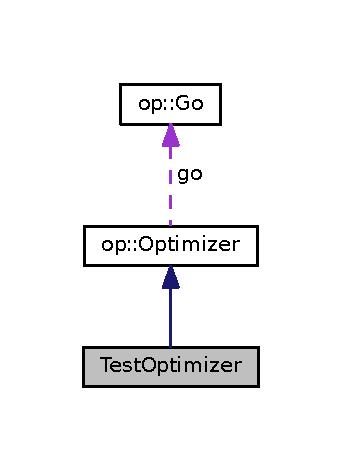
\includegraphics[width=164pt]{classTestOptimizer__coll__graph}
\end{center}
\end{figure}
\subsection*{Public Member Functions}
\begin{DoxyCompactItemize}
\item 
void \hyperlink{classTestOptimizer_acf4e70d78cbbb9dd44e002575d4477f7}{set\-Objective} (\hyperlink{classop_1_1Functional}{op\-::\-Functional} \&) override
\begin{DoxyCompactList}\small\item\em Sets the optimization objective. \end{DoxyCompactList}\item 
\hypertarget{classTestOptimizer_aaaaf8cea0b84a3327965dc89dfb2cd77}{double \hyperlink{classTestOptimizer_aaaaf8cea0b84a3327965dc89dfb2cd77}{Solution} () override}\label{classTestOptimizer_aaaaf8cea0b84a3327965dc89dfb2cd77}

\begin{DoxyCompactList}\small\item\em What to do when the solution is found. Return the objetive. \end{DoxyCompactList}\end{DoxyCompactItemize}
\subsection*{Additional Inherited Members}


\subsection{Detailed Description}


Definition at line 4 of file test\-\_\-optimizer.\-cpp.



\subsection{Member Function Documentation}
\hypertarget{classTestOptimizer_acf4e70d78cbbb9dd44e002575d4477f7}{\index{Test\-Optimizer@{Test\-Optimizer}!set\-Objective@{set\-Objective}}
\index{set\-Objective@{set\-Objective}!TestOptimizer@{Test\-Optimizer}}
\subsubsection[{set\-Objective}]{\setlength{\rightskip}{0pt plus 5cm}void Test\-Optimizer\-::set\-Objective (
\begin{DoxyParamCaption}
\item[{{\bf op\-::\-Functional} \&}]{o}
\end{DoxyParamCaption}
)\hspace{0.3cm}{\ttfamily [inline]}, {\ttfamily [override]}, {\ttfamily [virtual]}}}\label{classTestOptimizer_acf4e70d78cbbb9dd44e002575d4477f7}


Sets the optimization objective. 


\begin{DoxyParams}[1]{Parameters}
\mbox{\tt in}  & {\em o} & Objective Functional \\
\hline
\end{DoxyParams}


Implements \hyperlink{classop_1_1Optimizer_aace5e17d5ee0c38cd6f411d21dc2c3b0}{op\-::\-Optimizer}.



Definition at line 8 of file test\-\_\-optimizer.\-cpp.



The documentation for this class was generated from the following file\-:\begin{DoxyCompactItemize}
\item 
/usr/workspace/jekel1/\-Repos/op/src/test\-\_\-optimizer.\-cpp\end{DoxyCompactItemize}

\hypertarget{classop_1_1Variables_1_1VariableMap}{\section{op\-:\-:Variables\-:\-:Variable\-Map$<$ Variables, Field\-Type $>$ Class Template Reference}
\label{classop_1_1Variables_1_1VariableMap}\index{op\-::\-Variables\-::\-Variable\-Map$<$ Variables, Field\-Type $>$@{op\-::\-Variables\-::\-Variable\-Map$<$ Variables, Field\-Type $>$}}
}


Utility class for \char`\"{}converting\char`\"{} between Variables and something else.  




{\ttfamily \#include $<$op.\-hpp$>$}

\subsection*{Public Types}
\begin{DoxyCompactItemize}
\item 
\hypertarget{classop_1_1Variables_1_1VariableMap_a44075cd0bfdf6dff5f8c4ee67659addf}{using {\bfseries To\-Type\-Fn} = std\-::function$<$ Field\-Type(Variables \&)$>$}\label{classop_1_1Variables_1_1VariableMap_a44075cd0bfdf6dff5f8c4ee67659addf}

\item 
\hypertarget{classop_1_1Variables_1_1VariableMap_a02e59ee7e05d97048a745576a92af1f6}{using {\bfseries From\-Type\-Fn} = std\-::function$<$ Variables(Field\-Type \&)$>$}\label{classop_1_1Variables_1_1VariableMap_a02e59ee7e05d97048a745576a92af1f6}

\end{DoxyCompactItemize}
\subsection*{Public Member Functions}
\begin{DoxyCompactItemize}
\item 
\hypertarget{classop_1_1Variables_1_1VariableMap_a280fcad54e5f7417fec536ff795d6e48}{{\bfseries Variable\-Map} (To\-Type\-Fn to\-\_\-fn, From\-Type\-Fn from\-\_\-fn)}\label{classop_1_1Variables_1_1VariableMap_a280fcad54e5f7417fec536ff795d6e48}

\item 
\hypertarget{classop_1_1Variables_1_1VariableMap_a9c46abea1694e3337ab8608a20b71043}{Field\-Type {\bfseries convert\-From\-Variable} (Variables \&v)}\label{classop_1_1Variables_1_1VariableMap_a9c46abea1694e3337ab8608a20b71043}

\item 
\hypertarget{classop_1_1Variables_1_1VariableMap_a41e604a514cbadb13b613b3d35743c86}{Variables {\bfseries convert\-To\-Variable} (Field\-Type \&f)}\label{classop_1_1Variables_1_1VariableMap_a41e604a514cbadb13b613b3d35743c86}

\end{DoxyCompactItemize}
\subsection*{Protected Attributes}
\begin{DoxyCompactItemize}
\item 
\hypertarget{classop_1_1Variables_1_1VariableMap_ac9cfaff2e29e86c3bc4f6d9332ce9df7}{To\-Type\-Fn {\bfseries to\-Type\-\_\-}}\label{classop_1_1Variables_1_1VariableMap_ac9cfaff2e29e86c3bc4f6d9332ce9df7}

\item 
\hypertarget{classop_1_1Variables_1_1VariableMap_ab886321b3d16a4486f940eb7b7753bf4}{From\-Type\-Fn {\bfseries from\-Type\-\_\-}}\label{classop_1_1Variables_1_1VariableMap_ab886321b3d16a4486f940eb7b7753bf4}

\end{DoxyCompactItemize}


\subsection{Detailed Description}
\subsubsection*{template$<$class Variables, class Field\-Type$>$class op\-::\-Variables\-::\-Variable\-Map$<$ Variables, Field\-Type $>$}

Utility class for \char`\"{}converting\char`\"{} between Variables and something else. 

Definition at line 58 of file op.\-hpp.



The documentation for this class was generated from the following file\-:\begin{DoxyCompactItemize}
\item 
/usr/workspace/jekel1/\-Repos/op/src/op.\-hpp\end{DoxyCompactItemize}

\hypertarget{classop_1_1Vector}{\section{op\-:\-:Vector$<$ Vector\-Type $>$ Class Template Reference}
\label{classop_1_1Vector}\index{op\-::\-Vector$<$ Vector\-Type $>$@{op\-::\-Vector$<$ Vector\-Type $>$}}
}


Abstracted Optimization \hyperlink{classop_1_1Vector}{Vector} container.  




{\ttfamily \#include $<$op.\-hpp$>$}



Collaboration diagram for op\-:\-:Vector$<$ Vector\-Type $>$\-:
\nopagebreak
\begin{figure}[H]
\begin{center}
\leavevmode
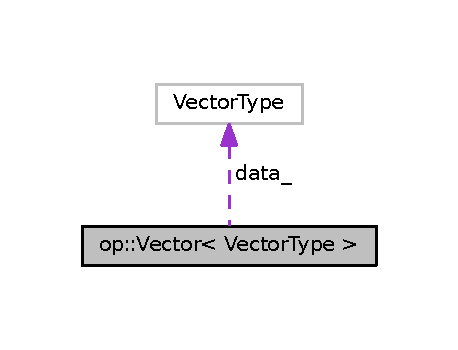
\includegraphics[width=220pt]{classop_1_1Vector__coll__graph}
\end{center}
\end{figure}
\subsection*{Public Types}
\begin{DoxyCompactItemize}
\item 
\hypertarget{classop_1_1Vector_ac28861996fd125f672dec63c9ec06c06}{using {\bfseries Scatter\-Fn} = std\-::function$<$ Vector\-Type()$>$}\label{classop_1_1Vector_ac28861996fd125f672dec63c9ec06c06}

\item 
\hypertarget{classop_1_1Vector_a99ef6a5d87839899f1daad6622a2e2fe}{using {\bfseries Gather\-Fn} = std\-::function$<$ Vector\-Type()$>$}\label{classop_1_1Vector_a99ef6a5d87839899f1daad6622a2e2fe}

\item 
\hypertarget{classop_1_1Vector_a00e1218c6eecc4290b4cda06f494ac84}{using {\bfseries Bounds\-Fn} = std\-::function$<$ Vector\-Type()$>$}\label{classop_1_1Vector_a00e1218c6eecc4290b4cda06f494ac84}

\end{DoxyCompactItemize}
\subsection*{Public Member Functions}
\begin{DoxyCompactItemize}
\item 
\hypertarget{classop_1_1Vector_aad3bc58b60937fb36f17343394701dd3}{{\bfseries Vector} (Vector\-Type \&\hyperlink{classop_1_1Vector_aa64decab605d7e408b8606fef7ddc8ea}{data}, Bounds\-Fn \hyperlink{classop_1_1Vector_a2a3ee86c58aaa32ccbd47aa0590cd108}{lower\-Bounds}, Bounds\-Fn \hyperlink{classop_1_1Vector_a5c5de10b7b946279045a92381638fcdd}{upper\-Bounds})}\label{classop_1_1Vector_aad3bc58b60937fb36f17343394701dd3}

\item 
\hypertarget{classop_1_1Vector_aa64decab605d7e408b8606fef7ddc8ea}{Vector\-Type \& \hyperlink{classop_1_1Vector_aa64decab605d7e408b8606fef7ddc8ea}{data} ()}\label{classop_1_1Vector_aa64decab605d7e408b8606fef7ddc8ea}

\begin{DoxyCompactList}\small\item\em Get the underlying data. \end{DoxyCompactList}\item 
\hypertarget{classop_1_1Vector_a2a3ee86c58aaa32ccbd47aa0590cd108}{Vector\-Type \hyperlink{classop_1_1Vector_a2a3ee86c58aaa32ccbd47aa0590cd108}{lower\-Bounds} ()}\label{classop_1_1Vector_a2a3ee86c58aaa32ccbd47aa0590cd108}

\begin{DoxyCompactList}\small\item\em Get the lower bounds for each local optimization variable. \end{DoxyCompactList}\item 
\hypertarget{classop_1_1Vector_a5c5de10b7b946279045a92381638fcdd}{Vector\-Type \hyperlink{classop_1_1Vector_a5c5de10b7b946279045a92381638fcdd}{upper\-Bounds} ()}\label{classop_1_1Vector_a5c5de10b7b946279045a92381638fcdd}

\begin{DoxyCompactList}\small\item\em Get the upper bounds for each local optimization variable. \end{DoxyCompactList}\end{DoxyCompactItemize}
\subsection*{Public Attributes}
\begin{DoxyCompactItemize}
\item 
\hypertarget{classop_1_1Vector_ac47f3f0d85652684bef9103225779248}{Gather\-Fn \hyperlink{classop_1_1Vector_ac47f3f0d85652684bef9103225779248}{gather}}\label{classop_1_1Vector_ac47f3f0d85652684bef9103225779248}

\begin{DoxyCompactList}\small\item\em Gather data function. \end{DoxyCompactList}\item 
\hypertarget{classop_1_1Vector_a6f7d9555e36785fd21fd1b5bf78f0632}{Scatter\-Fn \hyperlink{classop_1_1Vector_a6f7d9555e36785fd21fd1b5bf78f0632}{scatter}}\label{classop_1_1Vector_a6f7d9555e36785fd21fd1b5bf78f0632}

\begin{DoxyCompactList}\small\item\em Scatter data function. \end{DoxyCompactList}\end{DoxyCompactItemize}
\subsection*{Protected Attributes}
\begin{DoxyCompactItemize}
\item 
\hypertarget{classop_1_1Vector_a262d4f23576f1ecfc33ac3c25c3385be}{Bounds\-Fn {\bfseries lower\-Bounds\-\_\-}}\label{classop_1_1Vector_a262d4f23576f1ecfc33ac3c25c3385be}

\item 
\hypertarget{classop_1_1Vector_aa4b8f274aee871c3298d0bb16e96f1e0}{Bounds\-Fn {\bfseries upper\-Bounds\-\_\-}}\label{classop_1_1Vector_aa4b8f274aee871c3298d0bb16e96f1e0}

\item 
\hypertarget{classop_1_1Vector_ab3b8d6c893a35917ef5729e8cd3d7bf3}{Vector\-Type \& {\bfseries data\-\_\-}}\label{classop_1_1Vector_ab3b8d6c893a35917ef5729e8cd3d7bf3}

\end{DoxyCompactItemize}


\subsection{Detailed Description}
\subsubsection*{template$<$class Vector\-Type$>$class op\-::\-Vector$<$ Vector\-Type $>$}

Abstracted Optimization \hyperlink{classop_1_1Vector}{Vector} container. 

The intention is for the container to act as a general abstraction for optimization variables 

Definition at line 80 of file op.\-hpp.



The documentation for this class was generated from the following file\-:\begin{DoxyCompactItemize}
\item 
/usr/workspace/jekel1/\-Repos/op/src/op.\-hpp\end{DoxyCompactItemize}

\hypertarget{classop_1_1WaitLoop}{\section{op\-:\-:Wait\-Loop Class Reference}
\label{classop_1_1WaitLoop}\index{op\-::\-Wait\-Loop@{op\-::\-Wait\-Loop}}
}


{\ttfamily \#include $<$op\-\_\-waitloop.\-hpp$>$}

\subsection*{Public Types}
\begin{DoxyCompactItemize}
\item 
\hypertarget{classop_1_1WaitLoop_af0132a11722653e4f7b2d6bd3f214497}{using {\bfseries Constraint\-Action\-Fn} = std\-::function$<$ void(int)$>$}\label{classop_1_1WaitLoop_af0132a11722653e4f7b2d6bd3f214497}

\item 
\hypertarget{classop_1_1WaitLoop_ac64e8a4081d0d17040dfd714b76b289f}{using {\bfseries Unknown\-Action\-Fn} = std\-::function$<$ void(int)$>$}\label{classop_1_1WaitLoop_ac64e8a4081d0d17040dfd714b76b289f}

\end{DoxyCompactItemize}
\subsection*{Public Member Functions}
\begin{DoxyCompactItemize}
\item 
\hypertarget{classop_1_1WaitLoop_ab956a772dedd652f3ac4202fa79465e3}{{\bfseries final\-\_\-obj\-\_\-} (final\-\_\-obj)}\label{classop_1_1WaitLoop_ab956a772dedd652f3ac4202fa79465e3}

\item 
\hypertarget{classop_1_1WaitLoop_a964c8dcb4648f993cd5077fd2f3ddb5b}{{\bfseries comm\-\_\-} (comm)}\label{classop_1_1WaitLoop_a964c8dcb4648f993cd5077fd2f3ddb5b}

\item 
\hypertarget{classop_1_1WaitLoop_a907de1966578ce11ae28df8ae8ee776b}{\hyperlink{classop_1_1WaitLoop}{Wait\-Loop} \& \hyperlink{classop_1_1WaitLoop_a907de1966578ce11ae28df8ae8ee776b}{on\-Update} (const \hyperlink{namespaceop_af8b17abb60b9f5c60c0a6764d5aa1228}{Action\-Fn} \&update)}\label{classop_1_1WaitLoop_a907de1966578ce11ae28df8ae8ee776b}

\begin{DoxyCompactList}\small\item\em Set action to perform in Update state. \end{DoxyCompactList}\item 
\hypertarget{classop_1_1WaitLoop_ade829f1843983d3c283835a3f679a328}{\hyperlink{classop_1_1WaitLoop}{Wait\-Loop} \& \hyperlink{classop_1_1WaitLoop_ade829f1843983d3c283835a3f679a328}{on\-Objective\-Grad} (const \hyperlink{namespaceop_af8b17abb60b9f5c60c0a6764d5aa1228}{Action\-Fn} \&obj\-\_\-grad)}\label{classop_1_1WaitLoop_ade829f1843983d3c283835a3f679a328}

\begin{DoxyCompactList}\small\item\em Set action to perform in Objective Grad state. \end{DoxyCompactList}\item 
\hypertarget{classop_1_1WaitLoop_aafedafeb2d596a571608f76d2dbae2f9}{\hyperlink{classop_1_1WaitLoop}{Wait\-Loop} \& \hyperlink{classop_1_1WaitLoop_aafedafeb2d596a571608f76d2dbae2f9}{on\-Objective\-Eval} (const \hyperlink{namespaceop_af8b17abb60b9f5c60c0a6764d5aa1228}{Action\-Fn} \&obj\-\_\-eval)}\label{classop_1_1WaitLoop_aafedafeb2d596a571608f76d2dbae2f9}

\begin{DoxyCompactList}\small\item\em Set action to perform in Objective Eval state. \end{DoxyCompactList}\item 
\hypertarget{classop_1_1WaitLoop_aadebe2316999a2cfb9dc6dd25a23bf0e}{\hyperlink{classop_1_1WaitLoop}{Wait\-Loop} \& \hyperlink{classop_1_1WaitLoop_aadebe2316999a2cfb9dc6dd25a23bf0e}{on\-Constraints\-Eval} (const Constraint\-Action\-Fn \&constraints\-\_\-states)}\label{classop_1_1WaitLoop_aadebe2316999a2cfb9dc6dd25a23bf0e}

\begin{DoxyCompactList}\small\item\em Set action to perform in Constraint Eval state. \end{DoxyCompactList}\item 
\hypertarget{classop_1_1WaitLoop_a36342ba05f774307b760d394f72ae28e}{\hyperlink{classop_1_1WaitLoop}{Wait\-Loop} \& \hyperlink{classop_1_1WaitLoop_a36342ba05f774307b760d394f72ae28e}{on\-Constraints\-Grad} (const Constraint\-Action\-Fn \&constraints\-\_\-grad\-\_\-states)}\label{classop_1_1WaitLoop_a36342ba05f774307b760d394f72ae28e}

\begin{DoxyCompactList}\small\item\em Set action to perform in Constraint Grad state. \end{DoxyCompactList}\item 
\hypertarget{classop_1_1WaitLoop_acd4493e0c35a825b9e67241ab5283c2d}{\hyperlink{classop_1_1WaitLoop}{Wait\-Loop} \& \hyperlink{classop_1_1WaitLoop_acd4493e0c35a825b9e67241ab5283c2d}{on\-Solution} (const \hyperlink{namespaceop_af8b17abb60b9f5c60c0a6764d5aa1228}{Action\-Fn} \&solution\-\_\-state)}\label{classop_1_1WaitLoop_acd4493e0c35a825b9e67241ab5283c2d}

\begin{DoxyCompactList}\small\item\em Set action to perform in Solution state. \end{DoxyCompactList}\item 
\hypertarget{classop_1_1WaitLoop_a850572325e547f4c075ab9c90c027c24}{\hyperlink{classop_1_1WaitLoop}{Wait\-Loop} \& \hyperlink{classop_1_1WaitLoop_a850572325e547f4c075ab9c90c027c24}{on\-Unknown} (const Unknown\-Action\-Fn \&unknown\-\_\-state)}\label{classop_1_1WaitLoop_a850572325e547f4c075ab9c90c027c24}

\begin{DoxyCompactList}\small\item\em Set action to perform in Unknown state. \end{DoxyCompactList}\item 
\hypertarget{classop_1_1WaitLoop_ae3b247bb891c2b207c3c6fefd94891b5}{void {\bfseries operator()} ()}\label{classop_1_1WaitLoop_ae3b247bb891c2b207c3c6fefd94891b5}

\end{DoxyCompactItemize}
\subsection*{Public Attributes}
\begin{DoxyCompactItemize}
\item 
\hypertarget{classop_1_1WaitLoop_a94f0800799cc0ffc3db304e5b97ed709}{\hyperlink{classop_1_1WaitLoop_a94f0800799cc0ffc3db304e5b97ed709}{\-\_\-\-\_\-pad0\-\_\-\-\_\-}\-: get\-\_\-size\-\_\-(get\-\_\-size)}\label{classop_1_1WaitLoop_a94f0800799cc0ffc3db304e5b97ed709}

\begin{DoxyCompactList}\small\item\em Construct \hyperlink{classop_1_1WaitLoop}{Wait\-Loop}. \end{DoxyCompactList}\end{DoxyCompactItemize}
\subsection*{Protected Attributes}
\begin{DoxyCompactItemize}
\item 
\hypertarget{classop_1_1WaitLoop_a642bd1b3e47036c5568cbb6b6787a4b9}{std\-::function$<$ int()$>$ {\bfseries get\-\_\-size\-\_\-}}\label{classop_1_1WaitLoop_a642bd1b3e47036c5568cbb6b6787a4b9}

\item 
\hypertarget{classop_1_1WaitLoop_a4f1464ba44577c8020b92f7d93d112e0}{double \& {\bfseries final\-\_\-obj\-\_\-}}\label{classop_1_1WaitLoop_a4f1464ba44577c8020b92f7d93d112e0}

\item 
\hypertarget{classop_1_1WaitLoop_a79b4e513e0364b74e4614344d796c08a}{M\-P\-I\-\_\-\-Comm {\bfseries comm\-\_\-}}\label{classop_1_1WaitLoop_a79b4e513e0364b74e4614344d796c08a}

\item 
\hypertarget{classop_1_1WaitLoop_a0d96cc7db72e83fe4febe4feeb191c02}{\hyperlink{namespaceop_af8b17abb60b9f5c60c0a6764d5aa1228}{Action\-Fn} {\bfseries update\-\_\-}}\label{classop_1_1WaitLoop_a0d96cc7db72e83fe4febe4feeb191c02}

\item 
\hypertarget{classop_1_1WaitLoop_ab43f0a743f328462d3174dab0605a1c3}{\hyperlink{namespaceop_af8b17abb60b9f5c60c0a6764d5aa1228}{Action\-Fn} {\bfseries obj\-\_\-grad\-\_\-}}\label{classop_1_1WaitLoop_ab43f0a743f328462d3174dab0605a1c3}

\item 
\hypertarget{classop_1_1WaitLoop_ae85cfe7224b2abf09c2ff9fc0bd74ff6}{\hyperlink{namespaceop_af8b17abb60b9f5c60c0a6764d5aa1228}{Action\-Fn} {\bfseries obj\-\_\-eval\-\_\-}}\label{classop_1_1WaitLoop_ae85cfe7224b2abf09c2ff9fc0bd74ff6}

\item 
\hypertarget{classop_1_1WaitLoop_a04d5649624578117a6ea04939770c657}{Constraint\-Action\-Fn {\bfseries constraints\-\_\-states\-\_\-}}\label{classop_1_1WaitLoop_a04d5649624578117a6ea04939770c657}

\item 
\hypertarget{classop_1_1WaitLoop_a76263e0f6047570a229b2f5affdd8866}{Constraint\-Action\-Fn {\bfseries constraints\-\_\-grad\-\_\-states\-\_\-}}\label{classop_1_1WaitLoop_a76263e0f6047570a229b2f5affdd8866}

\item 
\hypertarget{classop_1_1WaitLoop_ae1fba8044d614753621d9708d57a3eaa}{\hyperlink{namespaceop_af8b17abb60b9f5c60c0a6764d5aa1228}{Action\-Fn} {\bfseries solution\-\_\-state\-\_\-}}\label{classop_1_1WaitLoop_ae1fba8044d614753621d9708d57a3eaa}

\item 
\hypertarget{classop_1_1WaitLoop_a5374e795b5358bbb394b4b5644e92538}{Unknown\-Action\-Fn {\bfseries unknown\-\_\-state\-\_\-}}\label{classop_1_1WaitLoop_a5374e795b5358bbb394b4b5644e92538}

\end{DoxyCompactItemize}


\subsection{Detailed Description}
A functor-\/pattern for serial\-Optimizer Wait\-Loops Follows the Fluent interface pattern 

Definition at line 35 of file op\-\_\-waitloop.\-hpp.



The documentation for this class was generated from the following file\-:\begin{DoxyCompactItemize}
\item 
/usr/workspace/jekel1/\-Repos/op/src/op\-\_\-waitloop.\-hpp\end{DoxyCompactItemize}

%--- End generated contents ---

% Index
\newpage
\phantomsection
\addcontentsline{toc}{part}{Index}
\printindex

\end{document}
